\documentclass[
	%parspace, % Add vertical space between paragraphs
	%noindent, % No indentation of first lines in each paragraph
	%nohyp, % No hyphenation of words
	%twoside, % Double sided format
	%draft, % Quicker draft compilation without rendering images
	%final, % Set final to hide todos
]{elteikthesis}[2024/05/10]

% The minted package is also supported for source highlighting
% See elteikthesis_minted.tex for example
%\usepackage[newfloat]{minted}

\usepackage{lscape}
\usepackage{pdflscape}
\usepackage{hyperref}

% Document's metadata
\title{GymBuddy edzésterv készítő, és követő alkalmazás} % title
\date{2023} % year of defense

% Author's metadata
\author{Nagy Arnold Alarik}
\degree{programtervező informatikus BSc}

% Superivsor(s)' metadata
\supervisor{Dr. Bernát Péter} % internal supervisor's name
\affiliation{egyetemi adjunktus} % internal supervisor's affiliation
%\extsupervisor{Külső Kornél} % external supervisor's name
%\extaffiliation{informatikai igazgató} % external supervisor's affiliation

% University's metadata
\university{Eötvös Loránd Tudományegyetem} % university's name
\faculty{Informatikai Kar} % faculty's name
\department{Programozáselmélet és Szoftvertechnológiai\\ Tanszék} % department's name
\city{Budapest} % city
\logo{elte_cimer_szines} % logo

% Add bibliography file
\addbibresource{elteikthesis.bib}

% The document
\begin{document}

% Set document language
\documentlang{hungarian}
%\documentlang{english}

% List of todos (not in the final document)
%\listoftodos[\todolabel]

% Title page (mandatory)
\maketitle
% Topic declaration page (mandatory) - can also be attached instead
%\includepdf{temabejelento.pdf}

% Table of contents (mandatory)
\tableofcontents
\cleardoublepage

% Main content
\chapter{Bevezetés}
\label{ch:bevezetes}

\section{Dolgozat felépítése}

\begin{description}
\item[I. Bevezetés:] Ebben a fejezetben részletesen kifejtem a szakdolgozat témáját, valamint bemutatom annak hátterét és motivációját.

\item[II. Felhasználói dokumentáció:] Ez a rész szolgál a program használatba vételéhez szükséges információkkal. Kiemelten foglalkozom a programkövetelményekkel, valamint az oldal funkcióinak részletes leírásával, melyeket képernyőképek és egy oldaltérkép segít megérteni.

\item[III. Fejlesztői dokumentáció:] Ez a rész a weboldal funkcióinak részletes elemzésére és leírására összpontosít. Usecase diagramok és User-story táblázatok segítségével világosan bemutatom a funkcionalitásokat. Továbbá részletesen tárgyalom a fejlesztés során alkalmazott keretrendszereket, tervezési mintákat, adatbázis felépítést és adattípusokat. A fejezet végén megtalálható a weboldal lokális futtatásához szükséges követelmények és lépéssorozat, valamint a tesztelési terv is.

\item[IV. Összefoglalás:] Ebben a záró fejezetben összegzem a szakdolgozatban megvalósított feladatot és annak eredményeit. Továbbá kitérek a lehetséges továbbfejlesztési lehetőségekre.

\item[V. Hivatkozások:] Az utolsó fejezetben felsorolom a szakdolgozat elkészítéséhez felhasznált programokat és dokumentációkat, valamint ezekre mutató hivatkozásokat.
\end{description}

\section{Témabejelentő}

A szakdolgozatom célja egy olyan telefonos/webes applikáció készítése, amelynek fő funkciója különböző edzéstervek készítése, valamint követése.

Lehetőség van klienseknek edzőkkel együttműködni egy belépési rendszer segítségével.
Az alkalmazás három fajta felhasználói fiókkal rendelkezik: Kliens, Edzői és Adminisztrációs.
A kliensek rögzíthetnek edzés során bizonyos adatokat az alkalmazásban, így lehetővé téve az edzéseik egyszerű követését.

A felhasználóknak rendelkezésre áll továbbá egy chat funkció is, amely használatával a kliensek képesek kommunikálni edzőkkel az alkalmazáson belül.
Edzéstervek könnyedén összeállíthatóak, akár az eddigi rögzített edzéstervek alapján automatikus válogatással.
Az adatok tárolása mögött egy központi adatbázis áll, így a felhasználó el tudja érni terveit, függetlenül a használt eszköztől.

Az alkalmazás e-mail értesítő rendszerrel is rendelkezik.
Lehetőség van az edzésterv pdf formátumban való exportálására, így akár ki is nyomtathatjuk azt.


\section{Motiváció}

Egyetemi éveim elején kezdtem erőemeléssel fogalkozni hobbiként, és igazán megragadott a sportág. Edzéseim mindig előre meg vannak tervezve edzőm közreműködésével, így segítve a gyors fejlődést, tapasztalt vagyok meglévő és gyakran használt eszközökkel amelyek edzés tervezési célra vannak használva világszerte. Az egyik ilyen elterjedt szoftver például egy egyszerű Excel-szerű táblázat, hiszen itt minden számadatot könnyedén rögzíteni tudunk, illetve különféle képletek alkalmazásával könnyíthetjük a munkánkat. Viszont számomra az ilyen szoftverek sok olyan funkcióval rendelkeznek, amelyeket használatuk során nem fogunk hasznosítani.

A probléma megoldása érdekében saját alkalmazást fejlesztettem, melyet úgy terveztem, hogy egyszerűsítse az edzők és kliensek munkáját az erőemelés terén. Az alkalmazás megkíméli őket a felesleges funkcióktól, ezzel optimalizálva a felhasználói élményt és hatékonyságot.
\cleardoublepage

% \chapter{Bevezetés}
\label{ch:intro}

Lorem ipsum dolor sit amet, consectetur adipiscing elit. In eu egestas mauris. Quisque nisl elit, varius in erat eu, dictum commodo lorem. Sed commodo libero et sem laoreet consectetur. Fusce ligula arcu, vestibulum et sodales vel, venenatis at velit \cite{dahl1972structured}. Aliquam erat volutpat. Proin condimentum accumsan velit id hendrerit. Cras egestas arcu quis felis placerat, ut sodales velit malesuada. Maecenas et turpis eu turpis placerat euismod.\footnote{Maecenas a urna viverra, scelerisque nibh ut, malesuada ex.}

Aliquam suscipit dignissim tempor. Praesent tortor libero, feugiat et tellus porttitor, malesuada eleifend felis. Orci varius natoque penatibus et magnis dis parturient montes, nascetur ridiculus mus \cite{cormen2009algorithms,krasner1988mvc}. Nullam eleifend imperdiet lorem, sit amet imperdiet metus pellentesque vitae. Donec nec ligula urna. Aliquam bibendum tempor diam, sed lacinia eros dapibus id. Donec sed vehicula turpis. Aliquam hendrerit sed nulla vitae convallis. Etiam libero quam, pharetra ac est nec, sodales placerat augue. \citeauthor{dijkstra1979goto} praesent eu consequat purus \cite{dijkstra1979goto}. 

% \cleardoublepage

\chapter{Felhasználói dokumentáció}
\label{ch:user}

\section{Rövid leírás, fogalmak}

Különböző felhasználói fiók típusok magyarázata:

\begin{itemize}
  \item Kliens: Az edzők által edzett kliensek rendelkeznek ilyen típusú fiókkal. Egy kliensnek egyszerre egy edzője lehet.
  \item Edző: Ők állítják őssze klienseik edzésterveit. Több klienssel is rendelkezhetnek.
  \item Adminisztrátor: Speciális adminisztrátori fiók, jogosultsággal rendelkezik a felhasználók listájának megtekintésére, valamint felhasználók törlésére. 
\end{itemize}

\bigskip

A weboldalon az \textbf{edzőknek} lehetőségük van \textbf{klienseik} számára ciklusokat\footnote[1]{A Ciklus egy összefoglaló név az olyan edzéstervekre, amelyek hetente ciklikusan ismétlődnek azonos gyakorlatokkal, több heten keresztül, hetenként eltérő nehézséggel} összeállítani. Egy ilyen \textbf{ciklus} több hétből állhat, hosszuk nem haladhatja meg a 6 hetet. Hetenként maximum 7 napra bonthatjuk az edzésterveket.
Egy adott napra több elvégzendő gyakorlatot rögzíthetünk, amelyeken a következő tényezőket állíthatjuk:
\begin{itemize}
  \item Gyakorlat neve
  \item Súly (weight)
  \item Szériák száma (series)
  \item Ismétlések száma (repetitions)
  \item Relatív nehézség (RPE)
\end{itemize}

\bigskip

Kliens felhasználók a saját névre szóló, edzőik által írt \textbf{ciklusaikat} elérik egy listában, az éppen aktív terveikben tudják módosítani az elvégzett gyakorlatok súly adatait, illetve a ténylegesen elvégzett \textbf{szériák}, \textbf{ismétlések} számát, illetve a tapasztalt \textbf{RPE} számot.

Kliensek edzőikkel kapcsolatba léphetnek egy beépített csevegő rendszer segítségével.

\section{Célközönség}

Az alkalmazás célközönsége azok, akik az erőemelés és más edzőtermi tevékenységek iránt érdeklődnek, és szeretnének fejlődni. Ide tartoznak azok, akik együttműködnének egy szakértő edzővel, valamint azok, akik edzői karriert szeretnének építeni a sportágban.

\section{Program használatához szükséges hardver- és szovtverkövetelmények}

A webapplikáció használatához egy friss verziójú böngészőprogramot futtatni képes hardverrel rendelkező eszközre van szükség, interneteléréssel.

A futtatáshoz ajánlott böngészők az alábbi felsorolt programok legfrissebb verziói, ezeken garantált az oldal helyes működése.
\begin{itemize}
  \item Google Chrome
  \item Mozilla Firefox
  \item Microsoft Edge
\end{itemize}

\bigskip

A futtatás során győződjünk meg arról, hogy böngészőprogramunkban engedélyezve van a JavaScript használata, mivel a felhasználói felület e technológiával van felépítve.

Az oldal reszponzív felhasználói felülettel rendelkezik, kisméretű kijelzőkön (minimum 375 pixel) is helyesen megjelenik, viszont a legjobb felhasználói élményhez legalább 1200 pixel széles kijelző ajánlott.

\section{Oldaltérkép}

\begin{figure}[H]
	\centering
	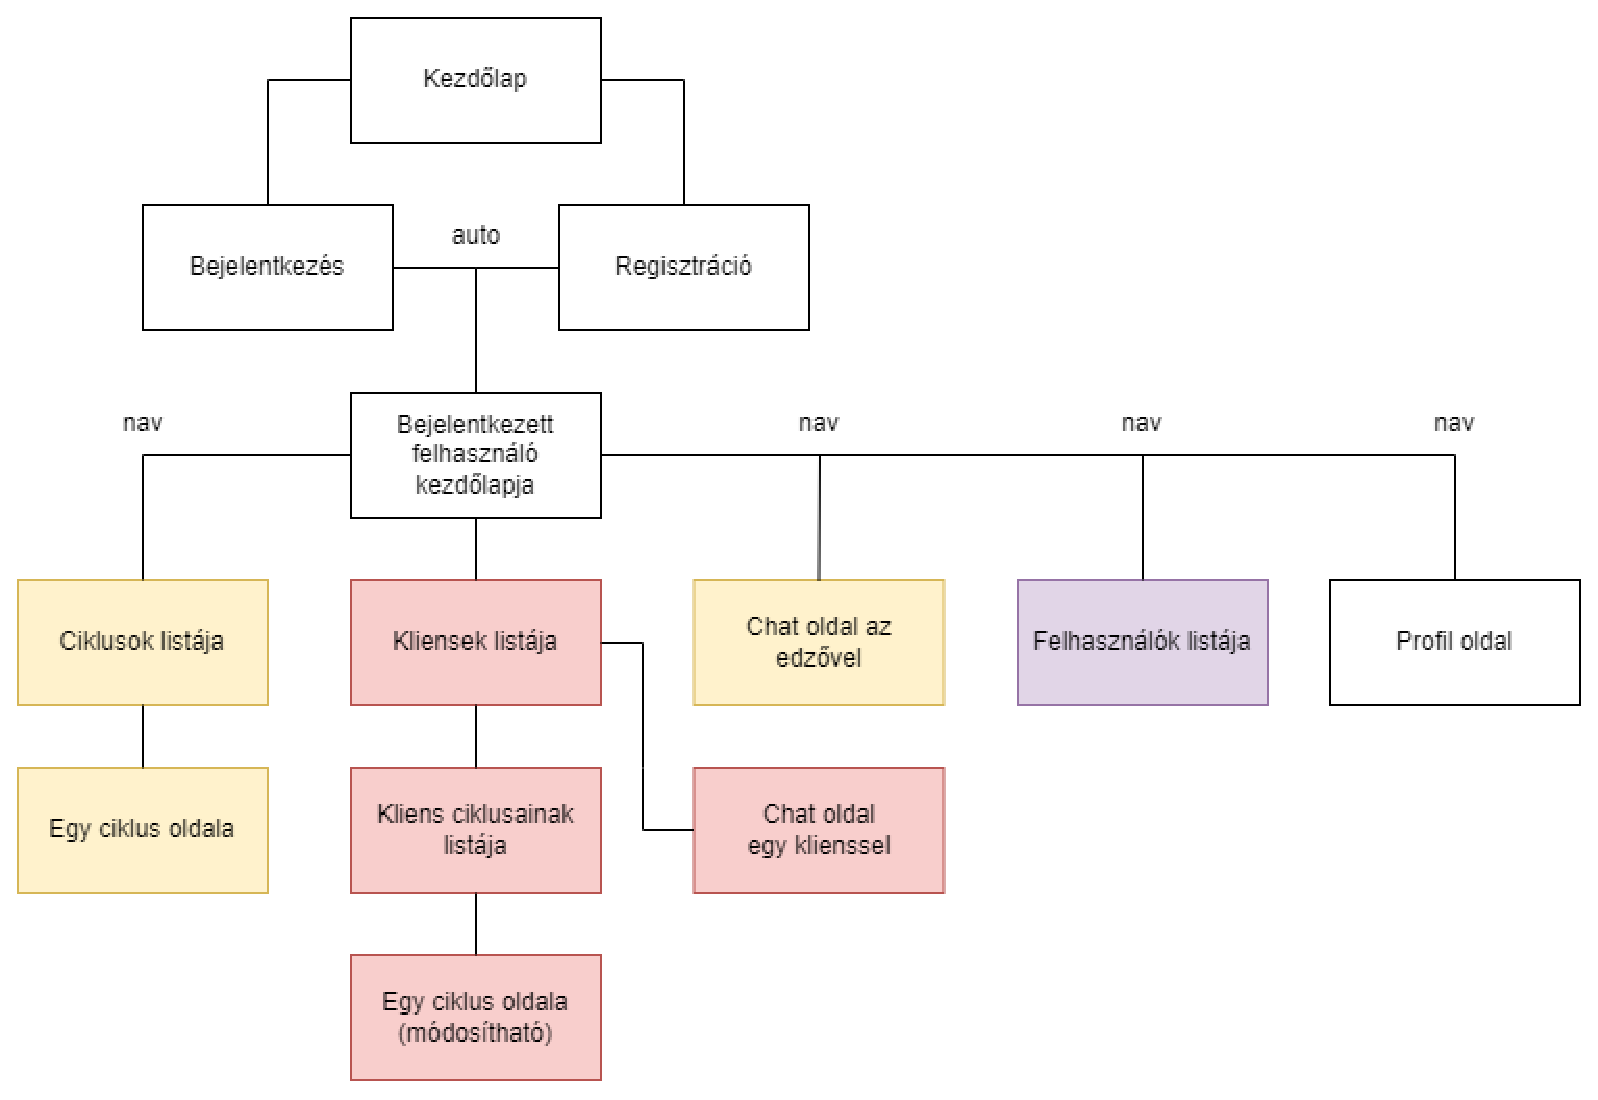
\includegraphics[width=1\linewidth]{oldalterkep}
	\caption{Oldaltérkép}
	\label{fig:oldalterkep}
\end{figure}

A \ref{fig:oldalterkep} ábrán a fehér kitöltésű mezők jelölik azokat az oldalakat, amelyeket bármilyen jogosultsággal rendelkező felhasználó képes elérni.
A citromsárga kitöltésű mezők a \textbf{kliens} jogosultsággal rendelkező felhasználó érheti el, a piros kitöltésűeket pedig \textbf{edző} típusú fiókkal lehetséges elérni.
A lila színű jelölés az \textbf{adminisztrátor} fiókok által elérhető oldalt jelöli.

A \textit{nav} kulcsszóval megjelölt útvonalak a navigációs menüből érhetőek el, az \textit{auto} kulcsszóval megjelöltek pedig automatikus átirányítás során, ha a felhasználó sikeresen bejelentkezett, vagy ha van bejelentkezett felhasználó eltárolva a készüléken.

\section{Weboldal funkcióinak bemutatása}

\subsection{Bevezetés}

Ebben az alfejezetben be fogom mutatni a webalkalmazás összes, felhasználók által elérhető oldalát, illetve kifejtem azok egyes funkcióit. Előszőr az összes, bejelentkezett felhasználó által elérhető oldalakat fogom bemutatni, majd rendre a \textbf{kliens}, \textbf{edző}, illetve \textbf{adminisztátor} jogosultságokkal elérhetőket.

\subsection{Kezdőlap}

\begin{figure}[H]
	\centering
	
\includegraphics[width=1\linewidth]{kezdolap}
	\caption{Kezdőlap}
	\label{fig:kezdolap}
\end{figure}

A \ref{fig:kezdolap} ábra mutatja a nem bejelentkezett felhasználóknak megjelenő kezdőlapot. A weboldal címe, rövid leírása látható. A jobb felső sarokban két gomb van elhejezve a felső navigációs sávban. A \textbf{Login} gomb megnyomásával a felhasználó a belejentkezési oldalra, a \textbf{Sign Up} gombra kattintással pedig a regisztrációs oldalra lesz átirányítva.

\subsection{Bejelentkezés}

\begin{figure}[H]
	\centering
	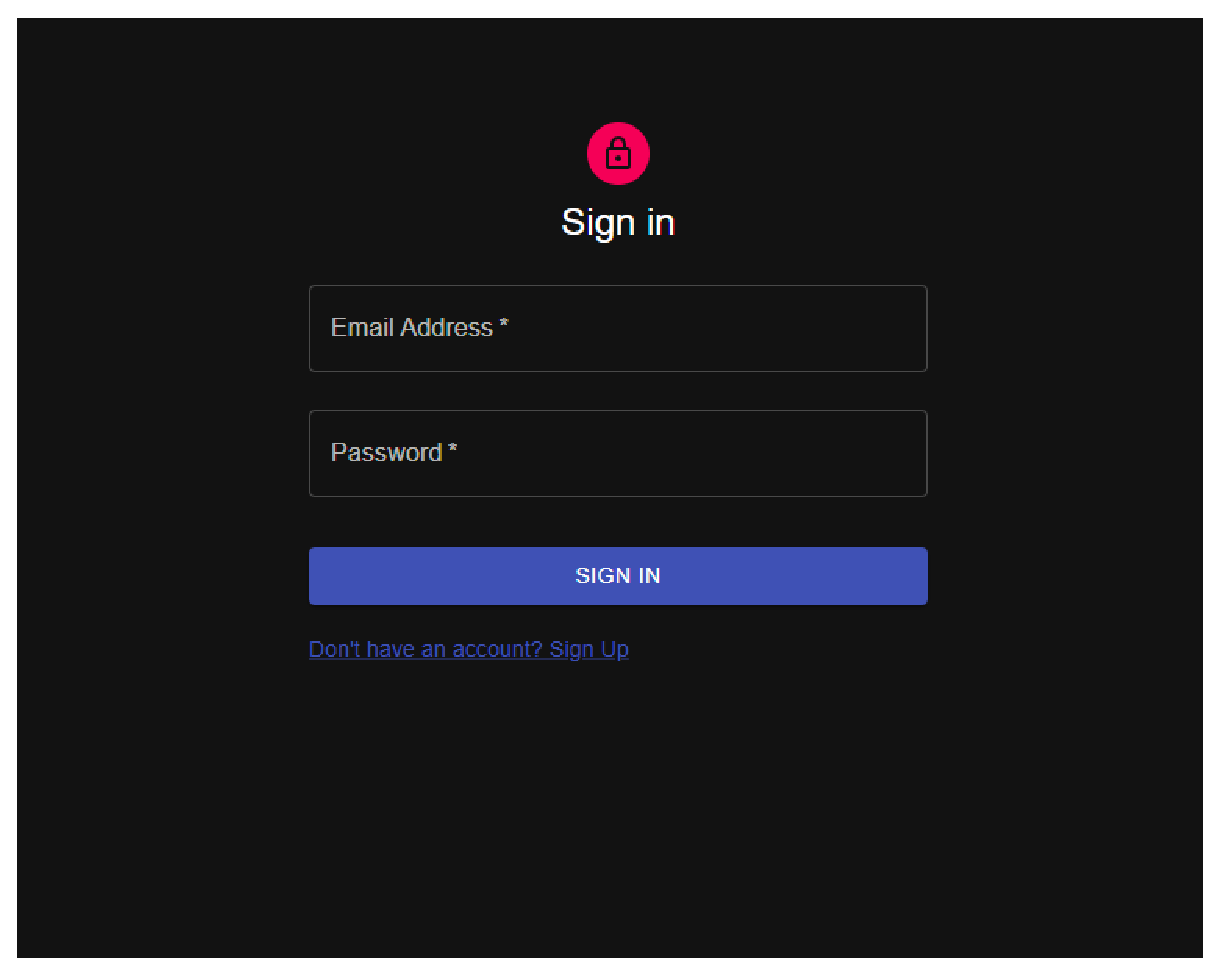
\includegraphics[width=1\linewidth]{login}
	\caption{Bejelentkezés}
	\label{fig:login}
\end{figure}

Az alkalmazásba funckiói eléréséhez előszőr be kell jelentkeznünk. Ezt a \ref{fig:login} ábrán látható oldalon tehetjük meg. A bejelentkezéshez meg kell adnunk a regisztrált fiókhoz tartozó email címet (Email Address) és jelszót (Password), majd a Sign In gomb megnyomásával a felhasználó a bejelentkezés után a kezdőlapra kerül, amennyiben helyes adatokat adott meg. Az oldal alján található link segítségével könnyedén át lehet kerülni a Regisztráció oldalra, amennyiben van már felhasználói fiókunk.

\subsection{Regisztráció}

\begin{figure}[H]
	\centering
	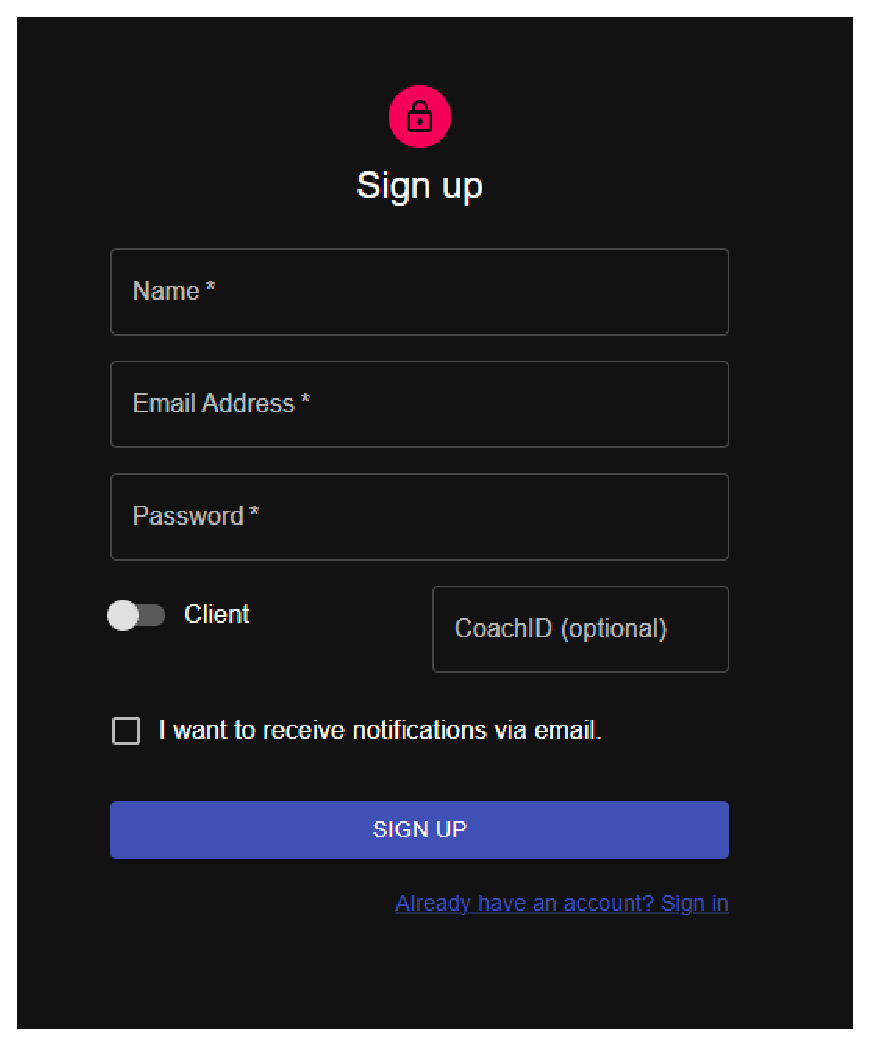
\includegraphics[width=0.6\linewidth]{register}
	\caption{Regisztráció}
	\label{fig:register}
\end{figure}

\begin{figure}[H]
	\centering
	
\includegraphics[width=0.6\linewidth]{registerslider}
	\caption{Regisztráció (edzői fiók)}
	\label{fig:registerslider}
\end{figure}

A felhasználói fiókunkat a \ref{fig:register} ábrán mutatott oldalon tudjuk létrehozni. Ezen az űrlapon ki kell töltenünk a fiókunk nevét (Name), ez fog megjelenni az alkalmazásban, mint felhasználónév. Meg kell adnunk egy email címet (Email Address), amelynek egy létező email címnek kell lennie. A jelszó (Password) mező kitöltése után van még lehetőségünk választani, hogy milyen típusú fiókot szeretnénk létrehozni. Kliens (Client) felhasználói fiók létrehozása esetén megadhatunk egy edző egyedi azonosítóját (CoachID), így regisztráció során is képesek vagyunk hozzárendelni fiókunkat egy edzőhöz. Edzői fiók létrehozása esetén hasonló bemeneti mező (\ref{fig:registerslider} ábra). Opcionálisan be tudjuk kapcsolni az email értesítéseket (I want to receive notifications via email). Bekapcsolása után a megadott email címen keresztül értesülni fogunk a regisztráció sikerességéről. Az űrlap elküldése után visszakerülünk a kezdőlapra, amennyiben nem történt hiba az adatok megadásával. Az oldal alján látható egy link, ennek megnyomásával átkerülünk a Bejelentkezés oldalra.

\subsection{Kezdőlap (kliens)}

\begin{figure}[H]
	\centering
	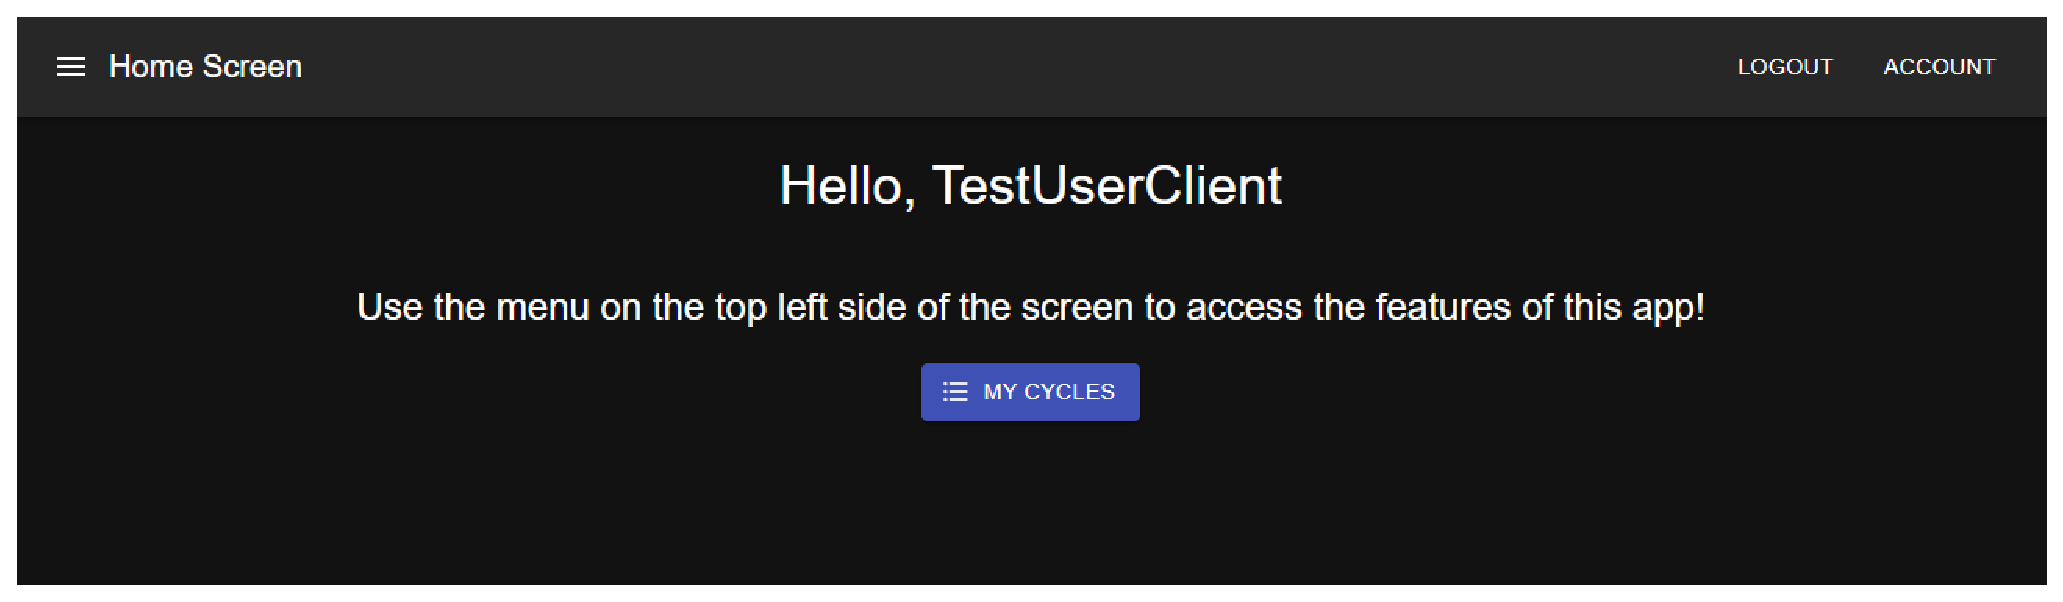
\includegraphics[width=1\linewidth]{kezdolapclient}
	\caption{Kezdőlap (kliens)}
	\label{fig:kezdolapclient}
\end{figure}

A \ref{fig:kezdolapclient} ábrán a Kezdőlap látató, ha a felhasználó kliens típusú fiókkal lép be az alkalmazásba. Az oldalon található egy gomb (My Cycles), amely a ciklusok listázó oldalára fogja átirányítani a felhasználót.

\subsection{Navigációs menü (kliens)}

\begin{figure}[H]
	\centering
	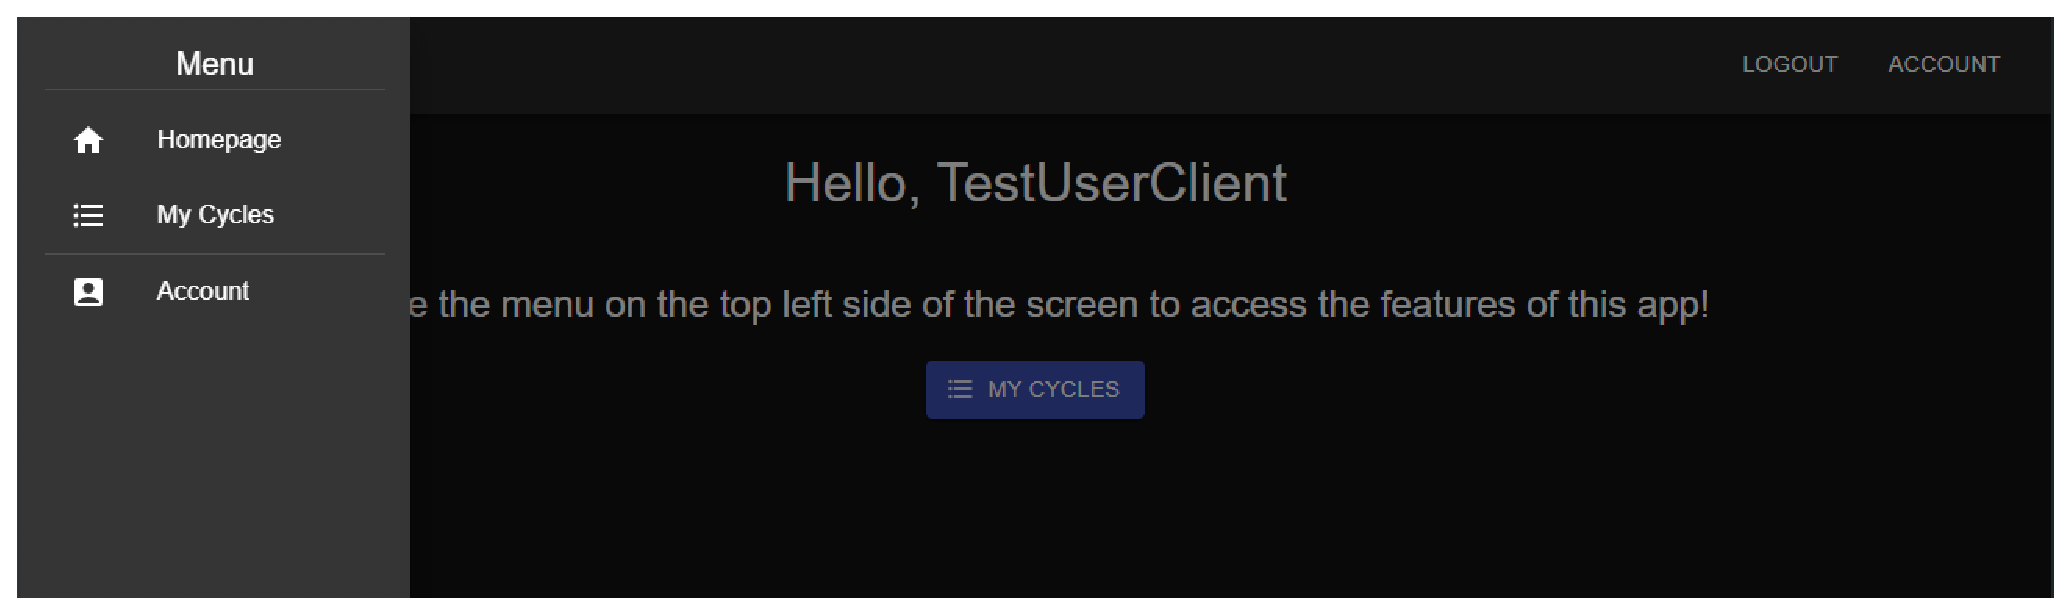
\includegraphics[width=1\linewidth]{navbarclient}
	\caption{Navigációs menü (kliens)}
	\label{fig:navbarclient}
\end{figure}

\begin{figure}[H]
	\centering
	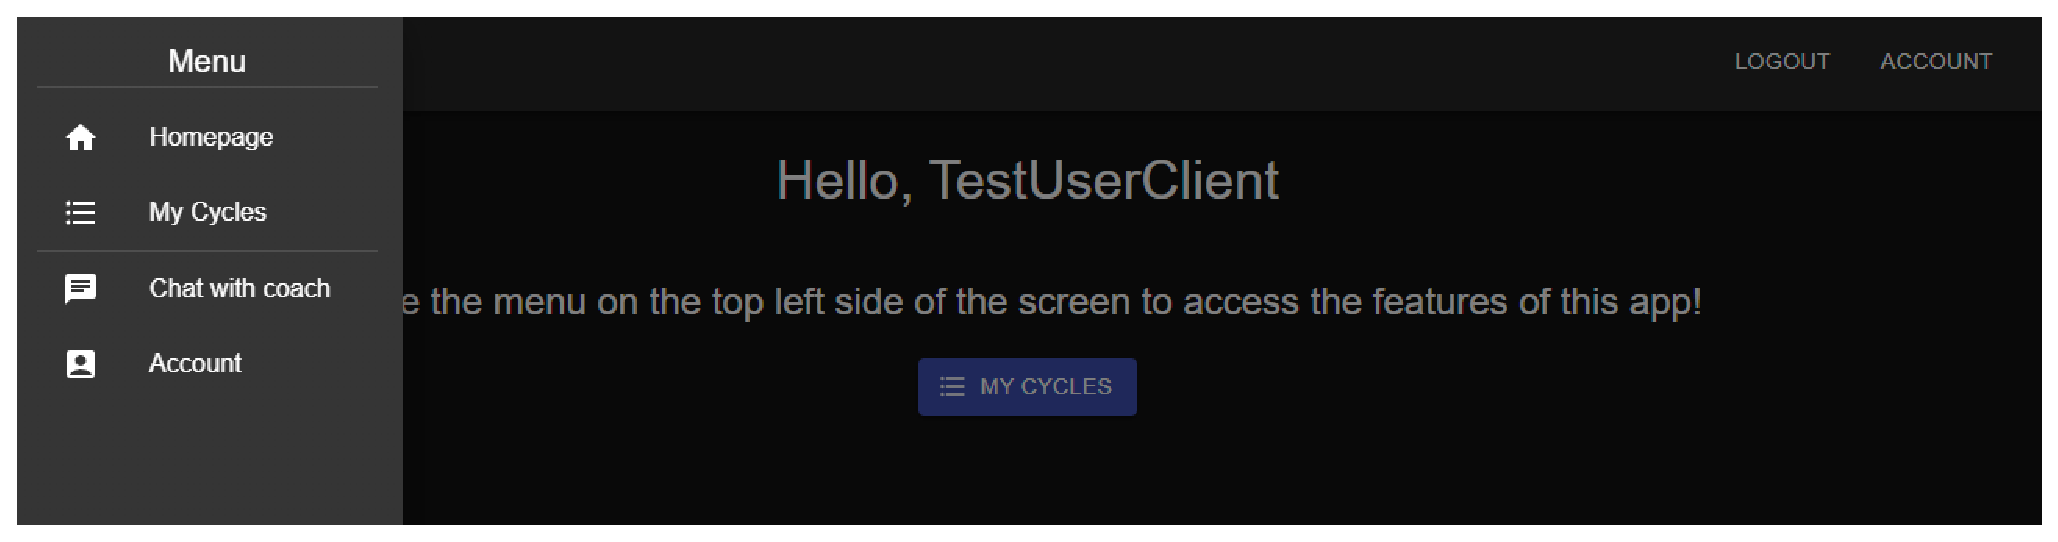
\includegraphics[width=1\linewidth]{navbarclienthascoach}
	\caption{Navigációs menü (kliens, rendelkezik edzővel)}
	\label{fig:navbarclienthascoach}
\end{figure}

A \ref{fig:navbarclient} ábrán a navigációs menü szerepel, kliens jogosultságokkal rendelkező fiókkal. A Homepage gombra kattintva visszakerülünk a kezdőlapra, a My Cycles gomb megnyomása után a ciklusok listázó oldalára kerülünk. \ref{fig:navbarclienthascoach} ábrán megfigyelhetjük, hogy amennyiben a kliens felhasználó rendelkezik edzővel, akihez hozzá van rendelve, lehetőség van a menüből megnyitni a két felhasználó közötti chat ablakot.

\subsection{Ciklusok listázó oldal (kliens)}

\begin{figure}[H]
	\centering
	\includegraphics[width=1\linewidth]{cyclesclient}
	\caption{Ciklusok listázó oldal (kliens)}
	\label{fig:cyclesclient}
\end{figure}

A fenti \ref{fig:cyclesclient} ábrán a ciklusok listázó oldala található, kliens nézetben. Itt találhatóak a különböző edzés ciklusok, amelyeket a felhasználó edzője készített. Felül találhatóak az aktív ciklusok (Active Cycles), amik szerkeszthetőek, illetve alul az inaktív ciklusok (Inactive Cycles), amelyeket nem tudunk szerkeszteni. Ennek a funkciónak lényege, hogy el tudjuk különíteni a már elvégzett, és az épp folyamatban lévő vagy még el nem kezdett ciklusokat. A cellákban a ciklusok neve mellett megjelenik még a létrehozásuk dátuma. Egy ilyen cellára kattintva átkerülünk az adott ciklus oldalára, ahol láthatjuk az edzéstervet.

\subsection{Ciklus/Edzésterv oldal (kliens)}

\begin{figure}[H]
	\centering
	\includegraphics[width=1\linewidth]{cycleclient}
	\caption{Ciklus/Edzésterv oldal (kliens)}
	\label{fig:cycleclient}
\end{figure}

\begin{figure}[H]
	\centering
	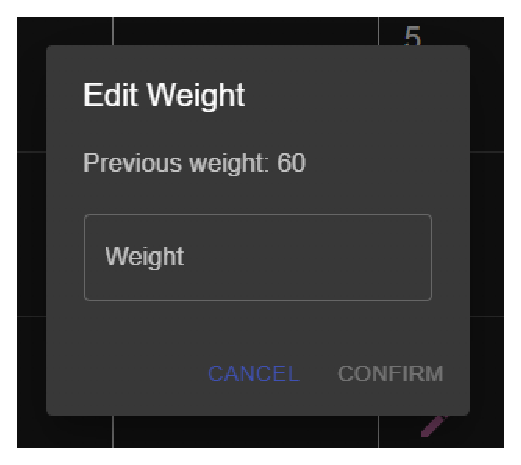
\includegraphics[width=0.4\linewidth]{editweight}
	\caption{Súly adat űrlapja}
	\label{fig:editweight}
\end{figure}

\begin{figure}[H]
	\centering
	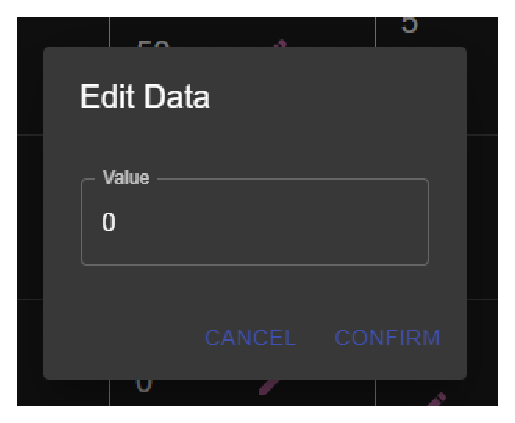
\includegraphics[width=0.4\linewidth]{editextrainfo}
	\caption{Ténylegesen elvégzett adat űrlapja}
	\label{fig:editextrainfo}
\end{figure}

A \ref{fig:cycleclient} ábrán látható egy ciklushoz tartozó edzéstervet tartalmazó oldal. A felső menüsáv alatt a jelenlegi nézetben lévő hétnek a száma található. Alatta bal oldalon egy gomb (Download PDF), amivel le tudjuk tölteni nyomtatható PDF formában a tervet. Az oldal közepén az edzésterv táblázata, napokra felosztva. A tervben a hetek között az egyes gyakorlatok közösek, viszont eltérhetnek súlyban, szériákban, ismétlésben és RPE számban. Az is állandó egy terven belül, hogy hány edzésnapból áll egy hét. Az oldal alján látható kék (vagy szürke, ha nem tudunk abban az irányban hetet váltani), nyíl ikonnal ellátott gomb megnyomásával a hetek között válthatunk. A jobb alsó sarokban lévő mentés ikonra kattintva (amíg nincs el nem mentett módosítás, szürke marad) az összes elvégzett módosítás elmentődik az adatbázisba.

A súly (Weight) oszlopban a ceruza ikonra kattintva a \ref{fig:editweight} ábrán látható űrlap jelenik meg. A bemeneti mezőbe egy nem negatív értéket írhatunk be, ezt az értéket a "Confirm" gombbal a táblázatba visszük.

A "Series", "Repetitions" és "RPE" oszlopokban is megjelennek ceruza ikonok, ezeknél az oszlopoknál a ténylegesen elvégzett értéket adhatjuk meg az adott gyakorlatra, amennyiben az eltérne az edző által kitűzött céltól. Itt szintén csak nem negatív értékeket adhatunk meg.

\subsection{Chat oldal (kliens)}

\begin{figure}[H]
	\centering
	\includegraphics[width=1\linewidth]{chatclient}
	\caption{Chat oldal (kliens)}
	\label{fig:chatclient}
\end{figure}

A chat oldal a fenti \ref{fig:chatclient} ábrán látható, ahol a kliens felhasználó üzenetet küldhet az edzőjének. A bejelentkezett felhasználó küldött üzenetei mindig a jobb oldalon jelennek meg kék háttérszínnel, míg csevegő társától kapott üzenetek pedig a bal oldalon, szürke színnel. Az üzenetek a jobb alsó sarokban lévő küldés gomb megnyomása, vagy az "ENTER" billentyű lenyomása után azonnal elküldésre kerülnek a másik fél számára, és valós időben meg is jelennek.

\subsection{Profil beállítások (kliens)}

\begin{figure}[H]
	\centering
	\includegraphics[width=1\linewidth]{accountpageclient}
	\caption{Profil beállítások (kliens)}
	\label{fig:accountpageclient}
\end{figure}

Megadott felhasználónév, jelszó megváltoztatására, illetve email értesítések ki/be kapcsolására a \ref{fig:accountpageclient} ábrán látható Profil beállítások oldalon van lehetőség. Bármilyen módosítás elmentéséhez meg kell adnunk a régi jelszavunkat a fiókhoz, amíg ez a mező üres, az űrlapot nem lehet elküldeni.

Az űrlapon a fentieken kívül megtekinthetünk különböző, fiókunkkal kapcsolatos információt, mint: megadott email cím, fiók létrehozásának dátuma, fiókunk típusa. Kliens felhasználók esetén az oldal kiírja edzőnk nevét, valamint a ciklusaink számát.

\subsection{Kezdőlap (edző)}

\begin{figure}[H]
	\centering
	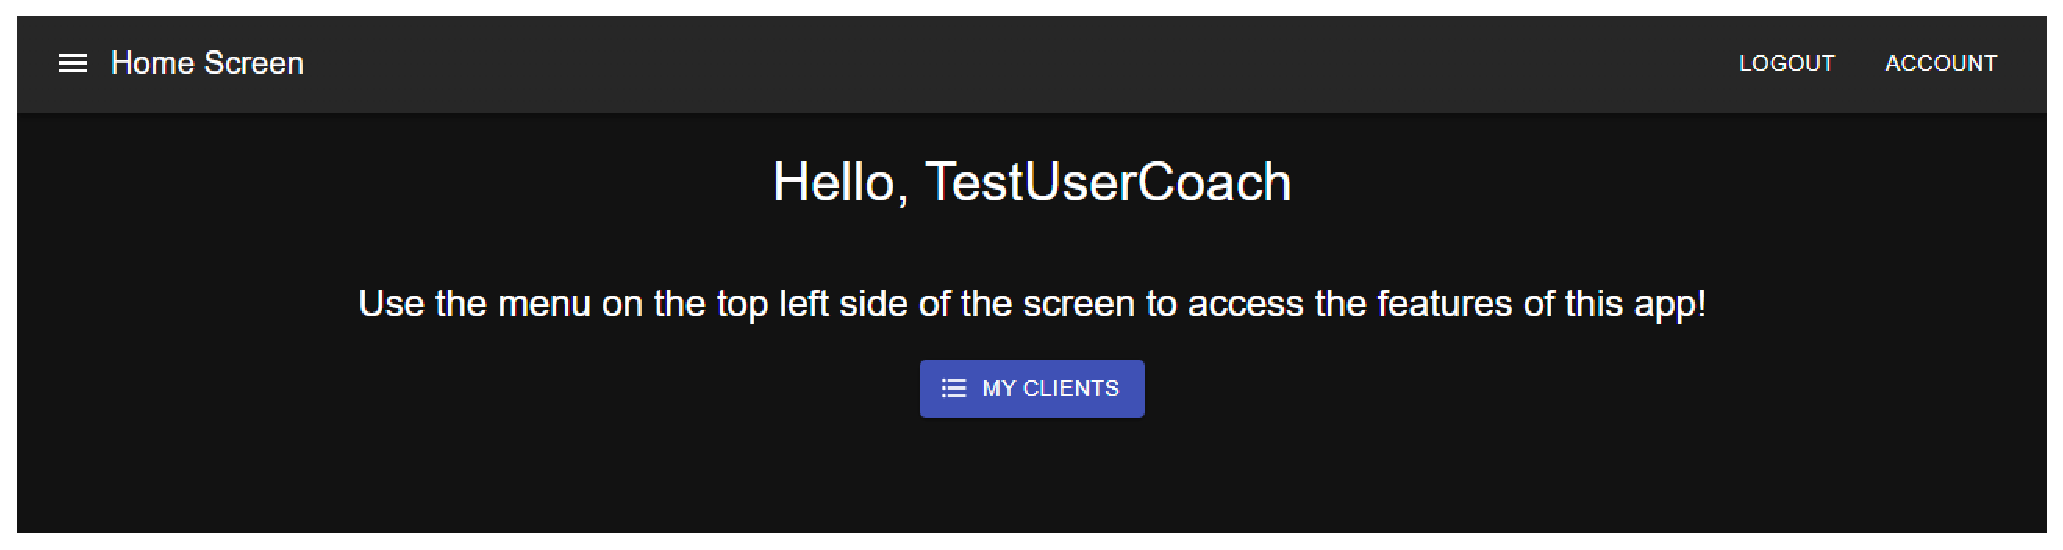
\includegraphics[width=1\linewidth]{kezdolapcoach}
	\caption{Kezdőlap (edző)}
	\label{fig:kezdolapcoach}
\end{figure}

A \ref{fig:kezdolapcoach} ábrán látható kezdőlap az edző jogosultsággal rendelkező fiókok esetén jelenik meg. A kliens fiókok kezdőlapjától csak annyiban tér el, hogy az oldalon található "My Clients" gomb az edző felhasználó klienseinek a listázó oldalára fog továbbítani.

\subsection{Kliensek listzázó oldal (edző)}

\begin{figure}[H]
	\centering
	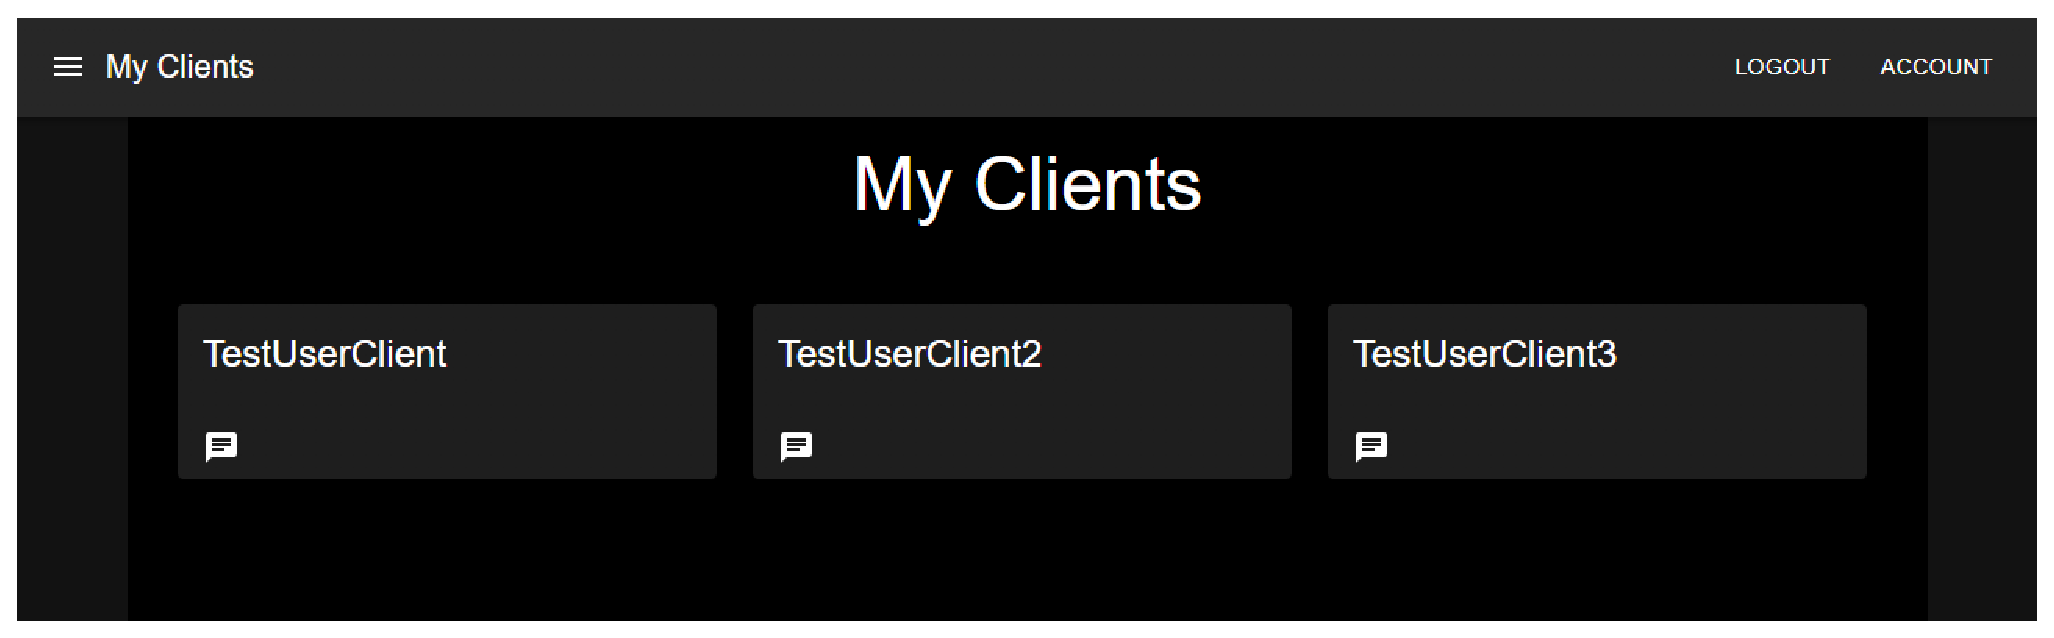
\includegraphics[width=1\linewidth]{clientspage}
	\caption{Kliensek listzázó oldal (edző)}
	\label{fig:clientspage}
\end{figure}

A \ref{fig:clientspage} ábrán megjelenő oldalon edző felhasználóknak a kliensek listázó oldala látható. Itt külön cellákban jelennek meg a felhasználó kliensei, felhasználónév alapján feltüntetve. Egy ilyen cellára kattintva átkerülünk az adott kliens ciklusainak listázó oldalára. A cellákban található egy chat ikon, ezt megnyomva az adott kliensnek tudunk üzeneteket küldeni, hasonlóan a \ref{fig:chatclient} ábrán látható felülethez.

\subsection{Kliens ciklusainak listázó oldala (edző)}

\begin{figure}[H]
	\centering
	\includegraphics[width=1\linewidth]{clientpage}
	\caption{Kliens ciklusainak listázó oldala (edző)}
	\label{fig:clientpage}
\end{figure}

Adott kliensünknek a ciklusait megtekinteni, módosítani, törölni, aktív státuszát megváltoztatni, illetve új ciklust létrehozni a \ref{fig:clientpage} ábrán lévő oldalon tudunk. Az oldal felépítése hasonló a kliens nézethez (\ref{fig:cyclesclient}), egy cellára kattintva szintén az adott ciklust tudjuk megtekinteni.

Ha ciklust szeretnénk törölni, a törlés gomb megnyomása után egy felugró ablakban a jóváhagyást követően a ciklus maradandóan törölve lesz az adatbázisból. Az archiválás ikonra kattintva pedig az aktív ciklust inaktívvá, az inaktívat aktívvá tudjuk tenni.

\subsection{Ciklus/edzésterv oldal (edző)}

\begin{figure}[H]
	\centering
	\includegraphics[width=1\linewidth]{cyclecoach}
	\caption{Ciklus/edzésterv oldal (edző)}
	\label{fig:cyclecoach}
\end{figure}

\begin{figure}[H]
	\centering
	\subcaptionbox{Gyakorlat hozzáadása űrlap}{
		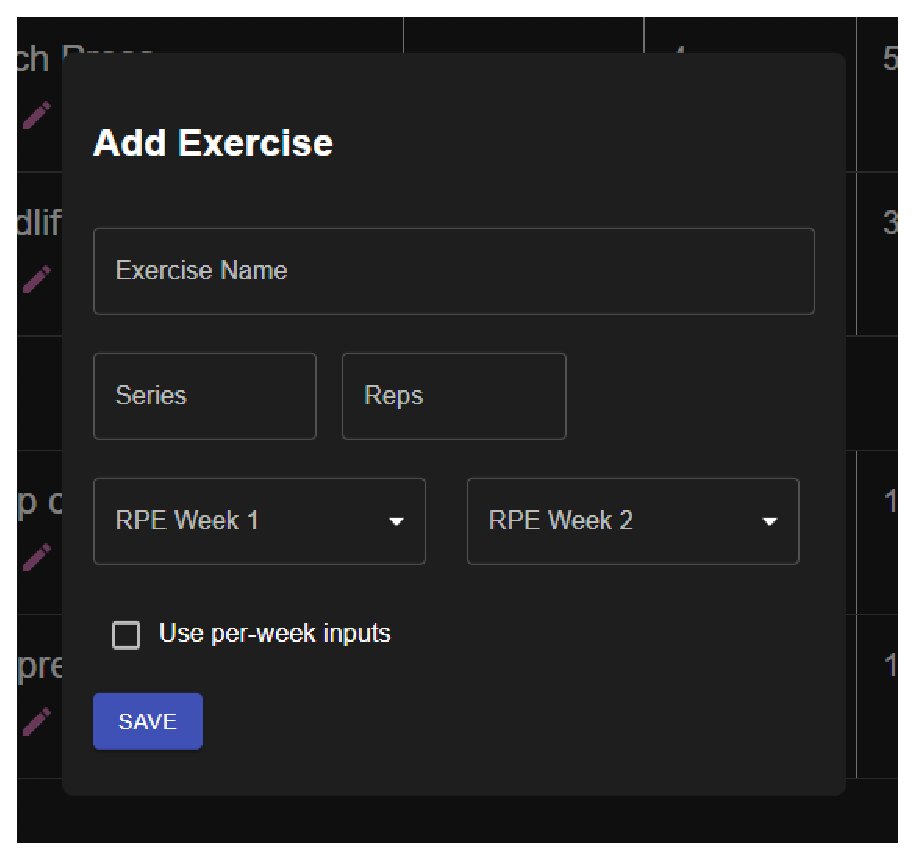
\includegraphics[width=0.45\linewidth]{addexercise}}
	\hspace{5pt}
	\subcaptionbox{Gyakorlat hozzáadása űrlap (hetenkénti bemenet)}{
		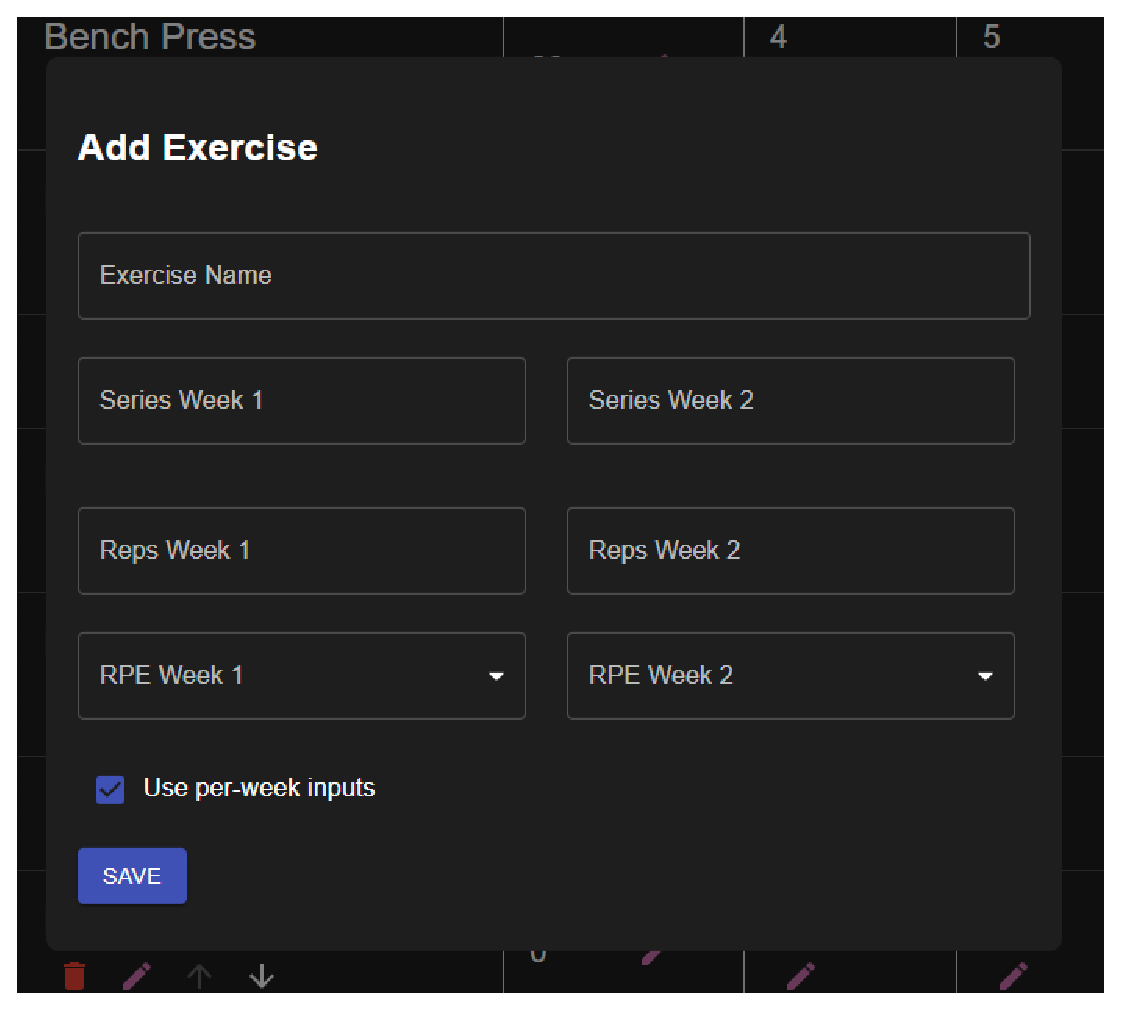
\includegraphics[width=0.45\linewidth]{addexerciseperweek}}
	\caption{Gyakorlat hozzáadása űrlapok}
	\label{fig:addrexercise}
\end{figure}

\begin{figure}[H]
	\centering
	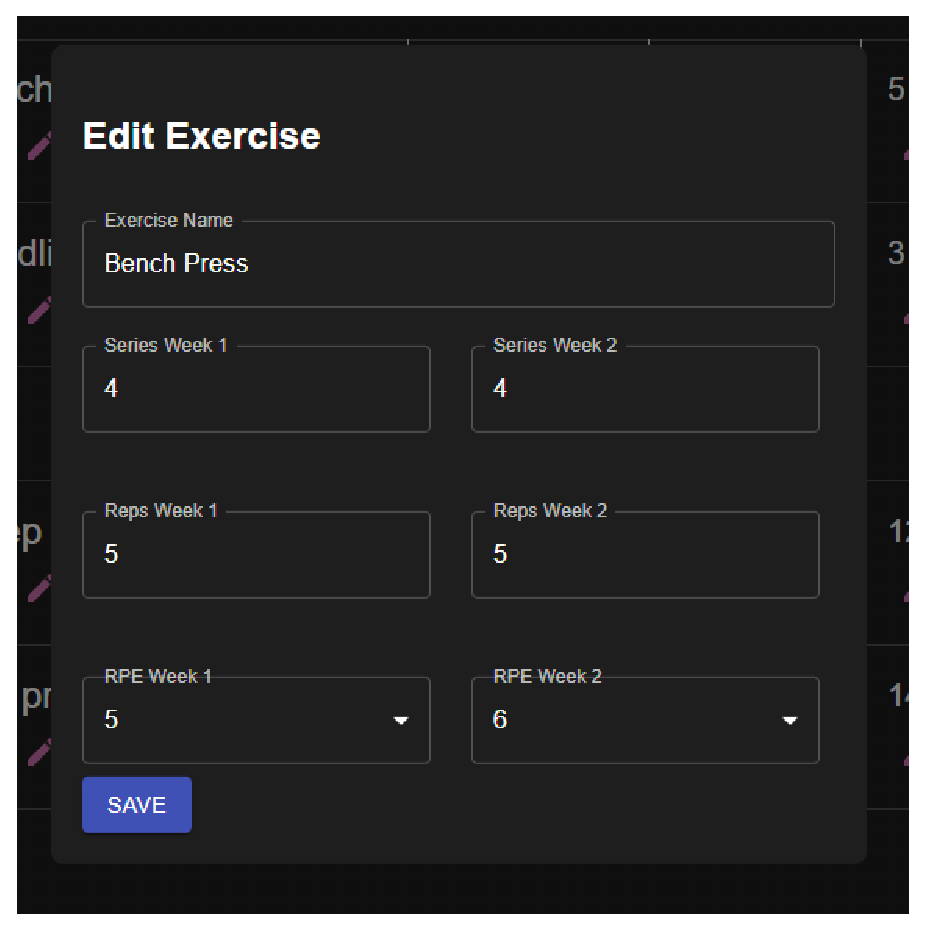
\includegraphics[width=0.6\linewidth]{editexercise}
	\caption{Gyakorlat módosítása űrlap}
	\label{fig:editexercise}
\end{figure}

\begin{figure}[H]
	\centering
	\subcaptionbox{RPE választó}{
		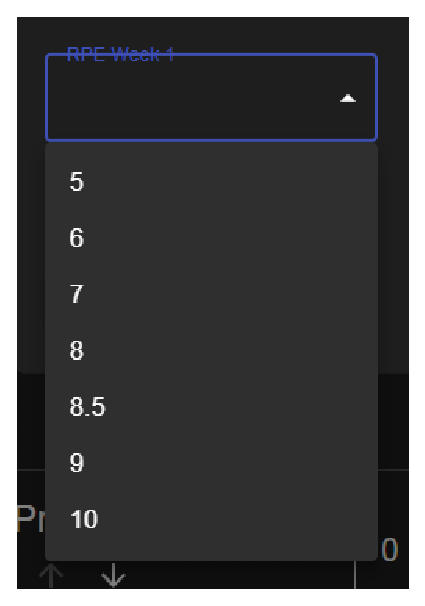
\includegraphics[width=0.3\linewidth]{rpeselector}}
	\hspace{5pt}
	\subcaptionbox{Új hét hozzáadása gomb}{
		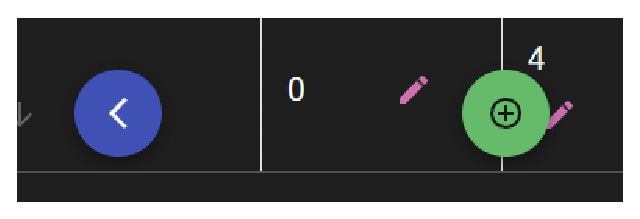
\includegraphics[width=0.3\linewidth]{addnewweek}}
	\caption{Egyéb bemenetek}
	\label{fig:addrexercise}
\end{figure}



Egy edzésterv megjelenítő oldal a \ref{fig:cyclecoach} számú ábrán látható módon jelenik meg. Hasonló a kliens nézethez, kibővítve sok adat módosító funkcióval. A funkciók magyarázatához feltről lefele fogok haladni.

\begin{description}
	\item[Hét törlése:] Az oldal tetején látható törlés ikonnal (hét száma felirat alatt) egy felugró ablak elfogadását követően törölni tudunk egy adott hetet a programból.
	\item[Gyakorlat törlése:] A gyakorlat neve alatt a törlés ikon kitörli a gyakorlatot a programból.
	\item[Gyakorlat módosítása:] A ceruza ikon segítségével gyakorlatokat tudunk módosítani, a módosító űrlapot a \ref{fig:editexercise} ábrán láthatjuk. Változtatni tudjuk a gyakorlat nevét, a szériákat, ismétlések számát és RPE számokat a ciklusban hetenként. A "Save" gomb megnyomásával felülírjuk a régi adatokat az űrlapban megadottakkal. RPE számot a \ref{fig:rpeselector} ábrán látható értékek közül választhatunk.
	\item[Gyakorlat mozgatása:] A nyíl ikonokkal a gyakorlatot tudjuk pakolni egy cellával feljebb vagy lejjebb az adott napon belül. Ez például akkor lehet fontos, ha előrébb szeretnénk vinni egy nehezebb gyakorlatot, amelyet majd könnyebbek követnek.
	\item[Súly módosítása:] Ha edzőként meg szeretnénk adni ajánlott súly mennyiséget egy gyakorlathoz, azt ezzel a gombbal megtehetjük (felülete és hatása megegyezik a \ref{fig:cycleclient} ábráról elmondottakkal).
	\item[Sorozatok/ismétlések/RPE módosítás:] A "Gyakorlat szerkesztése" űrlapon kívül az adott oszlophoz tartozó ceruza ikonra kattintva is meg tudjuk változtatni a gyakorlathoz rögzített adatokat, az űrlap megjelenése azonos a \ref{fig:editextrainfo} ábrával.
	\item[Nap törlése:] A nap száma melletti törlés gombra kattimtva az adott nap, összes gyakorlatával együtt törlésre kerül.
	\item[Gyakorlat hozzáadása:] Az adott naphoz tartozó gyakorlatok listája alatt egy újabb sorban látható egy hozzáadás gomb. Ennek megnyomásával felugrik a \ref{fig:addexercise} ábrán látható ablak. Meg kell adnunk a  gyakorlat nevét, illetve különböző információkat róla. A "Use per-week inputs" gombbal ki-be kapcsolhatjuk a hetenkénti bemenetet a szériák és ismétlések számára. Ezt azt jelenti, ha kikapcsoljuk a funkciót, a két bemeneten megadott szám hetenként meg fog egyezni a gyakorlaton. Ha be van kapcsolva, variálni tudjuk a hetek között az értékeket. Ennek célja, hogy egyszerűbbé tegye a sok gyakorlat rögzítését az edző felhasználóknak, ugyanis ciklusokon belül ezek az értékek általában megegyeznek. 
	\item[Nap hozzáadása:] A "Day" oszlop alján lévő plusz gombbal az edzéstervhez extra napot adhatunk.
	\item[Hetek közötti lapozás / mentés gomb:]  A nyilakkal hetek között válthatunk, a mentés gombbal pedig véglegesítjük a változtatásokat.
	\item[Új hét hozzáadása:] Ha el lapozunk a programban lévő utolsó hétre, a jobb oldali nyíl gomb egy plusz ikonra változik. Ennek megnyomásával és a felugró ablak elfogadásával új hét adódik a ciklushoz. 
\end{description}

Fontos megjegyezni, hogy ezen az oldalon történt változtatások véglegesítéséhez rá kell kattintani a mentés gombra, különben elvesznek.

\subsection{Profil beállítások (edző)}

\begin{figure}[H]
	\centering
	\includegraphics[width=1\linewidth]{accountpagecoach}
	\caption{Profil beállítások (edző)}
	\label{fig:accountpagecoach}
\end{figure}

Az edzői fiókhoz tartozó profil beállítások a \ref{fig:accountpagecoach} ábrán láthatóak. A beállítások nagy része azonos a \ref{fig:accountpageclient} ábrán láthatóakkal, kivéve az "Additional Information" fül alatt lévőket. Itt információt kapunk a mi (edző) azonosító kódunkról, amelyet klienseink regisztráció során meg tudnak adni. Ezen kívül a klienseink számát is megtekinthetjük.

\subsection{Felhasználók listája (adminisztrátor)}

\begin{figure}[H]
	\centering
	\includegraphics[width=1\linewidth]{manageusers}
	\caption{Felhasználók listája (adminisztrátor)}
	\label{fig:manageusers}
\end{figure}

A fenti \ref{fig:manageusers} ábrán az adminisztrátor felület látható. Ez a felhasználók kezelésére szolgál. Információkat láthatunk a fiók típusárol, az egyéni azonosítójukról, valamint a csatlakozási dátum is fel van tűntetve. Felhasználói fiókokat törölhetünk a "Delete User" gombbal, klienseket rendelhetünk edzőkhöz az "Add Client" gombbal, illetve ha lenyitjuk a "Clients" listát egy edző felhasználónak, klienseket is ki tudunk törölni az adott edzőhöz tartozó listából. Az oldalon a felül található menü használatával a különböző típusú fiókokra szűrhetjük a nézetet.

\pagebreak

\section{Megjelenő üzenetek}

A program használata során számos üzenet megjelenhet. Közöttük vannak hibaüzenetek, és visszaigazolás jellegűek. Típustól függetlenül az oldal bal alsó sarkában láthatóak, zöld vagy piros színnel, rendre ha visszaigazolás vagy hiba jellegűek.

\subsection{Tájékoztató üzenetek}


\cleardoublepage

% \chapter{User documentation}
\label{ch:user}

Lorem ipsum dolor sit amet $\mathbb{N}$\nomenclature{$\mathbb{N}$}{Set of natural numbers}, consectetur adipiscing elit. Duis nibh leo, dapibus in elementum nec, aliquet id sem. Suspendisse potenti. Nullam sit amet consectetur nibh. Donec scelerisque varius turpis at tincidunt. Cras a diam in mauris viverra vehicula. Vivamus mi odio, fermentum vel arcu efficitur, lacinia viverra nibh. Aliquam aliquam ante mi, vel pretium arcu dapibus eu. Nulla finibus ante vel arcu tincidunt, ut consectetur ligula finibus. Mauris mollis lectus sed ipsum bibendum, ac ultrices erat dictum. Suspendisse faucibus euismod lacinia $\mathbb{Z}$\nomenclature{$\mathbb{Z}$}{Set of integer numbers}.


\section{Enumerations and lists}

Etiam vel odio ante. Etiam pulvinar nibh quis massa auctor congue. Pellentesque quis odio vitae sapien molestie vestibulum sit amet et quam. Pellentesque vel dui eget enim hendrerit finibus at sit amet libero. Quisque sollicitudin ultrices enim, nec porta magna imperdiet vitae. Cras condimentum nunc dui, eget molestie nunc accumsan vel.

\begin{itemize}
	\item Fusce in aliquet neque, in pretium sem.
	\item Donec tincidunt tellus id lectus pretium fringilla.
	\item Nunc faucibus, erat pretium tempus tempor, tortor mi fringilla neque, ac congue ex dui vitae mauris.
\end{itemize}

Donec dapibus sodales ante, at scelerisque nunc laoreet sit amet. Mauris porttitor tincidunt neque, vel ullamcorper neque pulvinar et. Integer eu lorem euismod, faucibus lectus sed, accumsan felis. Nunc ornare mi at augue vulputate, eu venenatis magna mollis. Nunc sed posuere dui, et varius nulla. Sed mollis nibh augue, eget scelerisque eros ornare nec.

\begin{enumerate}
	\item\label{step:first} Donec pretium et quam a cursus. Ut sollicitudin tempus urna et mollis.
	\item Aliquam et aliquam turpis, sed fermentum mauris. Nulla eget ex diam.
	\item Donec eget tellus pharetra, semper neque eget, rutrum diam Step~\ref{step:first}.
\end{enumerate}

Praesent porta, metus eget eleifend consequat, eros ligula eleifend ex, a pellentesque mi est vitae urna. Vivamus turpis nunc, iaculis non leo eget, mattis vulputate tellus. Maecenas rutrum eros sem, pharetra interdum nulla porttitor sit amet. In vitae viverra ante. Maecenas sit amet placerat orci, sed tincidunt velit. Vivamus mattis, enim vel suscipit elementum, quam odio venenatis elit\footnote{Phasellus faucibus varius purus, nec tristique enim porta vitae.}, et mollis nulla nunc a risus. Praesent purus magna, tristique sed lacus sit amet, convallis malesuada magna. 

\begin{description}
	\item[Vestibulum venenatis] malesuada enim, ac auctor erat vestibulum et. Phasellus id purus a leo suscipit accumsan.
	\item[Orci varius natoque] penatibus et magnis dis parturient montes, nascetur ridiculus mus. Nullam interdum rhoncus nisl, vel pharetra arcu euismod sagittis. Vestibulum ac turpis auctor, viverra turpis at, tempus tellus.
	\item[Morbi dignissim] erat ut rutrum aliquet. Nulla eu rutrum urna. Integer non urna at mauris scelerisque rutrum sed non turpis.
\end{description}

\subsection{Lists with narrow spacing inbetween items}

Phasellus ultricies, sapien sit amet ultricies placerat, velit purus viverra ligula, id consequat ipsum odio imperdiet enim:
\begin{compactenum}
	\item Maecenas eget lobortis leo.
	\item Donec eget libero enim.
	\item In eu eros a eros lacinia maximus ullamcorper eget augue.
\end{compactenum}

\bigskip

In quis turpis metus. Proin maximus nibh et massa eleifend, a feugiat augue porta. Sed eget est purus. Duis in placerat leo. Donec pharetra eros nec enim convallis:
\begin{compactitem}
	\item Pellentesque odio lacus.
	\item Maximus ut nisl auctor.
	\item Sagittis vulputate lorem.
\end{compactitem}

\bigskip

Vestibulum ante ipsum primis in faucibus orci luctus et ultrices posuere cubilia Curae; Sed lorem libero, dignissim vitae gravida a, ornare vitae est.
\begin{compactdesc}
	\item[Cras maximus] massa commodo pellentesque viverra.
	\item[Morbi sit] amet ante risus. Aliquam nec sollicitudin mauris
	\item[Ut aliquam rhoncus sapien] luctus viverra arcu iaculis posuere
\end{compactdesc}


\section{Images and figures}

Aliquam vehicula luctus mi a pretium. Nulla quam neque, maximus nec velit in, aliquam mollis tortor. Aliquam erat volutpat. Curabitur vitae laoreet turpis. Integer id diam ligula. Nulla sodales purus id mi consequat, eu venenatis odio pharetra. Cras a arcu quam. Suspendisse augue risus, pulvinar a turpis et, commodo aliquet turpis. Nulla aliquam scelerisque mi eget pharetra. Mauris sed posuere elit, ac lobortis metus. Proin lacinia sit amet diam sed auctor. Nam viverra orci id sapien sollicitudin, a aliquam lacus suscipit, Figure~\ref{fig:example-1}:

\begin{figure}[H]
	\centering
	
\includegraphics[width=0.6\textwidth,height=100px]{elte_cimer_szines}
	\caption{Quisque ac tincidunt leo}
	\label{fig:example-1}
\end{figure}

\subsection{Framing figures}

Ut aliquet nec neque eget fermentum. Cras volutpat tellus sed placerat elementum. Quisque neque dui, consectetur nec finibus eget, blandit id purus. Nam eget ipsum non nunc placerat interdum.

\begin{figure}[H]
	\centering
	
\includegraphics[width=0.6\textwidth,height=100px,frame]{elte_cimer_szines}
	\caption{Quisque ac tincidunt leo}
\end{figure}

\subsection{Subfigures}

In non ipsum fermentum urna feugiat rutrum a at odio. Pellentesque habitant morbi tristique senectus et netus et malesuada fames ac turpis egestas. Nulla tincidunt mattis nisl id suscipit. Sed bibendum ac felis sed volutpat. Nam pharetra nisi nec facilisis faucibus. Aenean tristique nec libero non commodo. Nulla egestas laoreet tempus. Nunc eu aliquet nulla, quis vehicula dui. Proin ac risus sodales, gravida nisi vitae, efficitur neque, Figure~\ref{fig:example-2}:

\begin{figure}[H]
	\centering
	\subcaptionbox{Vestibulum quis mattis urna}{
		
\includegraphics[width=0.45\linewidth]{elte_cimer_szines}}
	\hspace{5pt}
	\subcaptionbox{Donec hendrerit quis dui sit amet venenatis}{
		
\includegraphics[width=0.45\linewidth]{elte_cimer_szines}}
	\caption{Aenean porttitor mi volutpat massa gravida}
	\label{fig:example-2}
\end{figure}

Nam et nunc eget elit tincidunt sollicitudin. Quisque ligula ipsum, tempor vitae tortor ut, commodo rhoncus diam. Pellentesque habitant morbi tristique senectus et netus et malesuada fames ac turpis egestas. Phasellus vehicula quam dui, eu convallis metus porta ac.


\section{Tables}

Nam magna ex, euismod nec interdum sed, sagittis nec leo. Nam blandit massa bibendum mattis tristique. Phasellus tortor ligula, sodales a consectetur vitae, placerat vitae dolor. Aenean consequat in quam ac mollis. 

\begin{table}[H]
	\centering
	\begin{tabular}{ | m{0.25\textwidth} | m{0.65\textwidth} | }
		\hline
		\textbf{Phasellus tortor} & \textbf{Aenean consequat} \\
		\hline \hline
		\emph{Sed malesuada} & Aliquam aliquam velit in convallis ultrices. \\
		\hline
		\emph{Purus sagittis} &  Quisque lobortis eros vitae urna lacinia euismod. \\
		\hline
		\emph{Pellentesque} & Curabitur ac lacus pellentesque, eleifend sem ut, placerat enim. Ut auctor tempor odio ut dapibus. \\
		\hline
	\end{tabular}
	\caption{Maecenas tincidunt non justo quis accumsan}
	\label{tab:example-1}
\end{table}

\subsection{Multi rows and multi columns}

Mauris a dapibus lectus. Vestibulum commodo nibh ante, ut maximus magna eleifend vel. Integer vehicula elit non lacus lacinia, vitae porttitor dolor ultrices. Vivamus gravida faucibus efficitur. Ut non erat quis arcu vehicula lacinia. Nulla felis mauris, laoreet sed malesuada in, euismod et lacus. Aenean at finibus ipsum. Pellentesque dignissim elit sit amet lacus congue vulputate.

\begin{table}[htb]
	\centering
	\begin{tabular}{ | c | r | r | r | r | r | r | }
		\hline
		\multirow{2}{*}{\textbf{Quisque}} & \multicolumn{2}{ c | }{\textbf{Suspendisse}} & \multicolumn{2}{ c | }{\textbf{Aliquam}} & \multicolumn{2}{ c | }{\textbf{Vivamus}} \\
		\cline{2-7}
		& Proin & Nunc & Proin & Nunc & Proin & Nunc \\
		\hline \hline		
		Leo & 2,80 MB & 100\% & 232 KB & 8,09\% & 248 KB & 8,64\% \\
		\hline
		Vel & 9,60 MB & 100\% & 564 KB & 5,74\% & 292 KB & 2,97\% \\
		\hline
		Auge & 78,2 MB & 100\% & 52,3 MB & 66,88\% & 3,22 MB & 4,12\% \\
		\hline 
	\end{tabular}
	\caption[Rövid cím a táblázatjegyzékbe]{Vivamus ac arcu fringilla, fermentum neque sed, interdum erat. Mauris bibendum mauris vitae enim mollis, et eleifend turpis aliquet.}
	\label{tab:example-2}
\end{table}

\subsection{Long tables over multiple pages}

Nunc porta placerat leo, sit amet porttitor dui porta molestie. Aliquam at fermentum mi. Maecenas vitae lorem at leo tincidunt volutpat at nec tortor. Vivamus semper lacus eu diam laoreet congue. Vivamus in ipsum risus. Nulla ullamcorper finibus mauris non aliquet. Vivamus elementum rhoncus ex ut porttitor.

\begin{center}
	\begin{longtable}{ | p{0.3\textwidth} | p{0.7\textwidth} | }
		
		\hline
		\multicolumn{2}{|c|}{\textbf{Praesent aliquam mauris enim}}
		\\ \hline
		
		\emph{Suspendisse potenti} & \emph{Lorem ipsum dolor sit amet}
		\\ \hline \hline
		\endfirsthead % table header on first page
		
		\hline
		\emph{Suspendisse potenti} & \emph{Lorem ipsum dolor sit amet}
		\\ \hline \hline
		\endhead % table header on further pages
		
		\hline
		\endfoot % table footer on previous pages
		
		\endlastfoot % table footer on last page
		
		\emph{Praesent}
		& Nulla ultrices et libero sit amet fringilla. Nunc scelerisque ante tempus sapien placerat convallis.
		\\ \hline
		
		\emph{Luctus}
		& Integer hendrerit erat massa, non hendrerit risus convallis at. Curabitur ultrices, justo in imperdiet condimentum, neque tortor luctus enim, luctus posuere massa erat vitae nibh.
		\\ \hline
		
		\emph{Egestas}
		& Duis fermentum feugiat augue in blandit. Mauris a tempor felis. Pellentesque ultricies tristique dignissim. Pellentesque aliquam semper tristique. Nam nec egestas dolor. Vestibulum id elit quis enim fringilla tempor eu a mauris. Aliquam vitae lacus tellus. Phasellus mauris lectus, aliquam id leo eget, auctor dapibus magna. Fusce lacinia felis ac elit luctus luctus.
		\\ \hline
		
		\emph{Dignissim}
		& Praesent aliquam mauris enim, vestibulum posuere massa facilisis in. Suspendisse potenti. Nam quam purus, rutrum eu augue ut, varius vehicula tellus. Fusce dui diam, aliquet sit amet eros at, sollicitudin facilisis quam. Phasellus tempor metus vel augue gravida pretium. Proin aliquam aliquam blandit. Nulla id tempus mi. Fusce in aliquam tortor.
		\\ \hline
		
		\emph{Pellentesque}
		& Donec felis nibh, imperdiet a arcu non, vehicula gravida nibh. Quisque interdum sapien eu massa commodo, ac elementum felis faucibus.
		\\ \hline
		
		\emph{Molestie}
		& Cras ullamcorper tellus et auctor ultricies. Maecenas tincidunt euismod lectus nec venenatis. Suspendisse potenti. Pellentesque pretium nunc ut euismod cursus. Nam venenatis condimentum quam. Curabitur suscipit efficitur aliquet. Interdum et malesuada fames ac ante ipsum primis in faucibus.
		\\ \hline
		
		\emph{Vivamus semper}
		& In purus purus, faucibus eu libero vulputate, tristique sodales nunc. Nulla ut gravida dolor. Fusce vel pellentesque mi, vel efficitur eros. Nunc vitae elit tellus. Sed vestibulum auctor consequat. 
		\\ \hline
		
		\emph{Condimentum}
		& Nulla scelerisque, leo et facilisis pretium, risus enim cursus turpis, eu suscipit ipsum ipsum in mauris. Praesent eget pulvinar ipsum, suscipit interdum nunc. Nam varius massa ut justo ullamcorper sollicitudin. Vivamus facilisis suscipit neque, eu fermentum risus. Ut at mi mauris.
		\\ \hline
		
		\caption{Praesent ullamcorper consequat tellus ut eleifend}
		\label{tab:example-3}		
	\end{longtable}
\end{center}
% \cleardoublepage


% \chapter{Developer documentation}
\label{ch:impl}

Lorem ipsum dolor sit amet, consectetur adipiscing elit. Duis nibh leo, dapibus in elementum nec, aliquet id sem. Suspendisse potenti. Nullam sit amet consectetur nibh. Donec scelerisque varius turpis at tincidunt.


\section{Theorem-like environments}

\begin{definition}
Mauris tristique sollicitudin ultrices. Etiam tristique quam sit amet metus dictum imperdiet. Nunc id lorem sed nisl pulvinar aliquet vitae quis arcu. Morbi iaculis eleifend porttitor.
\end{definition}

Maecenas rutrum eros sem, pharetra interdum nulla porttitor sit amet. In vitae viverra ante. Maecenas sit amet placerat orci, sed tincidunt velit. Vivamus mattis, enim vel suscipit elementum, quam odio venenatis elit, et mollis nulla nunc a risus. Praesent purus magna, tristique sed lacus sit amet, convallis malesuada magna. Phasellus faucibus varius purus, nec tristique enim porta vitae.

\begin{theorem}
Nulla finibus ante vel arcu tincidunt, ut consectetur ligula finibus. Mauris mollis lectus sed ipsum bibendum, ac ultrices erat dictum. Suspendisse faucibus euismod lacinia. Etiam vel odio ante.
\end{theorem}
\begin{proof}
Etiam pulvinar nibh quis massa auctor congue. Pellentesque quis odio vitae sapien molestie vestibulum sit amet et quam. Pellentesque vel dui eget enim hendrerit finibus at sit amet libero. Quisque sollicitudin ultrices enim, nec porta magna imperdiet vitae. Cras condimentum nunc dui.
\end{proof}

Donec dapibus sodales ante, at scelerisque nunc laoreet sit amet. Mauris porttitor tincidunt neque, vel ullamcorper neque pulvinar et. Integer eu lorem euismod, faucibus lectus sed, accumsan felis. 

\begin{remark}
Nunc ornare mi at augue vulputate, eu venenatis magna mollis. Nunc sed posuere dui, et varius nulla. Sed mollis nibh augue, eget scelerisque eros ornare nec. Praesent porta, metus eget eleifend consequat, eros ligula eleifend ex, a pellentesque mi est vitae urna. Vivamus turpis nunc, iaculis non leo eget, mattis vulputate tellus.
\end{remark}

Fusce in aliquet neque, in pretium sem. Donec tincidunt tellus id lectus pretium fringilla. Nunc faucibus, erat pretium tempus tempor, tortor mi fringilla neque, ac congue ex dui vitae mauris. Donec pretium et quam a cursus.

\begin{note}
Aliquam vehicula luctus mi a pretium. Nulla quam neque, maximus nec velit in, aliquam mollis tortor. Aliquam erat volutpat. Curabitur vitae laoreet turpis. Integer id diam ligula.
\end{note}

Ut sollicitudin tempus urna et mollis. Aliquam et aliquam turpis, sed fermentum mauris. Nulla eget ex diam. Donec eget tellus pharetra, semper neque eget, rutrum diam.

\subsection{Equations, formulas}

Duis suscipit ipsum nec urna blandit, $2 + 2 = 4$ pellentesque vehicula quam fringilla. Vivamus euismod, lectus sit amet euismod viverra, dolor metus consequat sapien, ut hendrerit nisl nulla id nisi. Nam in leo eu quam sollicitudin semper a quis velit.

$$a^2 + b^2 = c^2$$

Phasellus mollis, elit sed convallis feugiat, dolor quam dapibus nibh, suscipit consectetur lacus risus quis sem. Vivamus scelerisque porta odio, vitae euismod dolor accumsan ut.

In mathematica, identitatem Euleri (equation est scriptor vti etiam notum) sit aequalitatem Equation~\ref{eq:euler}:
\begin{equation}\label{eq:euler}
e^{i \times \pi} + 1 = 0
\end{equation}

Vestibulum ante ipsum primis in faucibus orci luctus et ultrices posuere cubilia curae; Nullam pulvinar purus at pharetra elementum.
Aequationes adsignans aequationis signum:
\begin{align}
	A & = \frac{\pi r^2}{2} \\
	& = \frac{1}{2} \pi r^2
\end{align}

Proin tempor risus a efficitur condimentum. Cras lobortis ligula non sollicitudin euismod. Fusce non pellentesque nibh, non elementum tellus.
Omissa numeratione aliquarum aequationum:
\begin{align}
	f(u) & =\sum_{j=1}^{n} x_jf(u_j) \nonumber \\
	& =\sum_{j=1}^{n} x_j \sum_{i=1}^{m} a_{ij}v_i \nonumber \\
	& =\sum_{j=1}^{n} \sum_{i=1}^{m} a_{ij}x_jv_i
\end{align}

\section{Source code samples}

Nulla sodales purus id mi consequat, eu venenatis odio pharetra. Cras a arcu quam. Suspendisse augue risus, pulvinar a turpis et, commodo aliquet turpis. Nulla aliquam scelerisque mi eget pharetra. Mauris sed posuere elit, ac lobortis metus. Proin lacinia sit amet diam sed auctor. Nam viverra orci id sapien sollicitudin, a aliquam lacus suscipit. Quisque ac tincidunt leo Code~\ref{src:cpp} and \ref{src:csharp}:

\lstset{caption={Hello World in C++}, label=src:cpp}
\begin{lstlisting}[language={C++}]
#include <stdio>

int main() 
{
	int c;
	std::cout << "Hello World!" << std::endl;

	std::cout << "Press any key to exit." << std::endl;
	std::cin >> c;
	
	return 0;
}
\end{lstlisting}

\lstset{caption={Hello World in C\#}, label=src:csharp}
\begin{lstlisting}[language={[Sharp]C}]
using System;
namespace HelloWorld
{
	class Hello 
	{
		static void Main() 
		{
			Console.WriteLine("Hello World!");
			
			Console.WriteLine("Press any key to exit.");
			Console.ReadKey();
		}
	}
}
\end{lstlisting}

\subsection{Algorithms}

A general Interval Branch and Bound algorithm is shown in Algorithm~\ref{alg:ibb}. An appropriate selection rule is applied in Step~\ref{step:selrule}.\\
Source of example: \href{https://www.inf.u-szeged.hu/actacybernetica/}{Acta Cybernetica (this is a hyperlink)}.

\begin{algorithm}[H]
\caption{A general interval B\&B algorithm} 
\label{alg:ibb} 
\textbf{\underline{Funct}} IBB($S,f$)
\begin{algorithmic}[1] % display line numbers before every n line, here n = 1
\State Set the working list ${\cal L}_W$ := $\{S\}$ and the final list ${\cal L}_Q$ := $\{\}$     
\While{( ${\cal L}_W \neq \emptyset$ )} \label{alg:igoend}
	\State  Select an interval $X$ from ${\cal L}_W$ \label{step:selrule}\Comment{Selection rule}  
	\State Compute $lbf(X)$ \Comment{Bounding rule}		  
	\If{$X$ cannot be eliminated} \Comment{Elimination rule}
		\State Divide $X$ into $X^j,\ j=1,\dots, p$, subintervals   \Comment{Division rule}
		\For{$j=1,\ldots,p$}
			\If{$X^j$ satisfies the termination criterion} \Comment{Termination rule}
				\State Store $X^j$ in ${\cal L}_W$ 
			\Else
				\State Store $X^j$ in ${\cal L}_W$ 
			\EndIf
		\EndFor  
	\EndIf
\EndWhile
\State \textbf{return} ${\cal L}_Q$
\end{algorithmic}
\end{algorithm}

% \cleardoublepage

\chapter{Fejlesztői dokumentáció}
\label{ch:implementation}

\section{Use-case diagramok}

\subsection{Kliens use-case diagram}

\begin{figure}[H]
	\centering
	\fbox{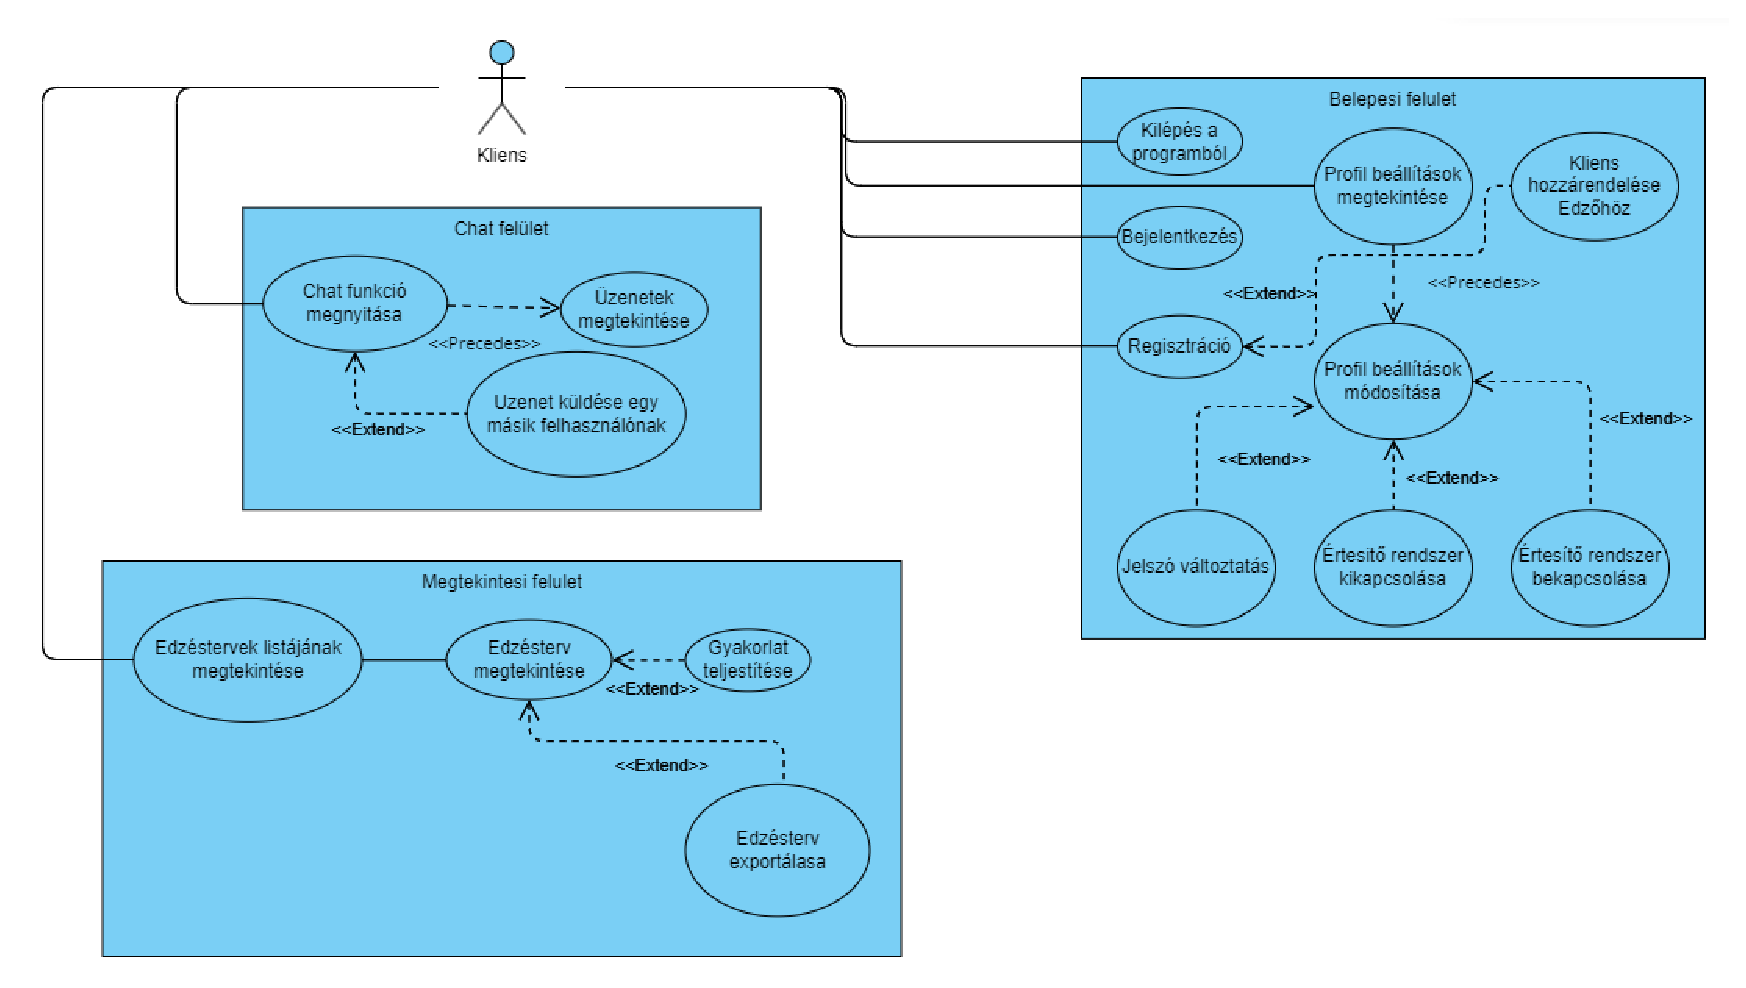
\includegraphics[width=0.97\linewidth]{usecaseclient}}
	\caption{Kliens use-case diagram (készült: Visual Paradigm Online \cite{visualparadigm} nevű programmal)}
	\label{fig:usecaseclient}
\end{figure}

\subsection{Edző use-case diagram}

\begin{figure}[H]
	\centering
	\fbox{\includegraphics[width=0.97\linewidth]{usecasecoach}}
	\caption{Edző use-case diagram (készült: Visual Paradigm Online \cite{visualparadigm} nevű programmal)}
	\label{fig:usecasecoach}
\end{figure}

Edzőknek elérhetőek a kliensek minden fő funkciója, a szerkesztési felület kialakítása hasonló a megtekintési felülethez, kiegészítve szerkesztésre vonatkozó funckiókkal.

\subsection{Adminisztrátor use-case diagram}

\begin{figure}[H]
	\centering
	\fbox{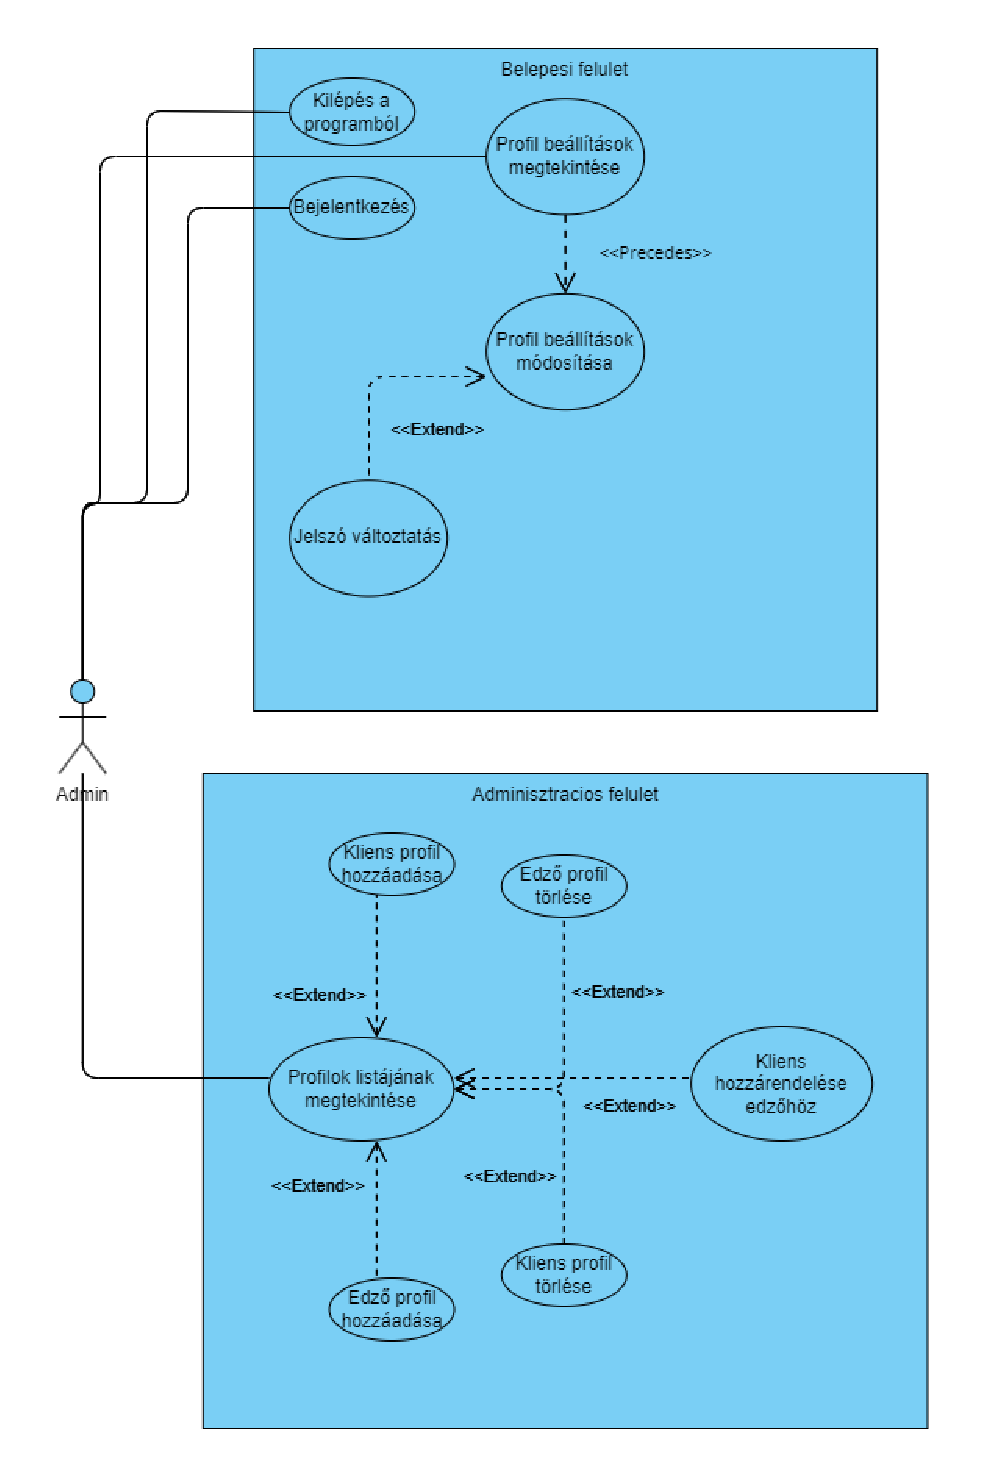
\includegraphics[width=0.8\linewidth]{usecaseadmin}}
	\caption{Adminisztrátor use-case diagram (készült: Visual Paradigm Online \cite{visualparadigm} nevű programmal)}
	\label{fig:usecaseadmin}
\end{figure}

Adminisztrátorként nem elérhetőek a kliens és edző felhasználók funkciói. Egy adminisztrátor csupán a felhasználókat tudja kezelni (törölni, klienseket hozzárendelni edzőkhöz).

\section{User-story táblázatok}

% Latogato userstory

\begin{center}
	\begin{longtable}{ | p{0.06\textwidth} | p{0.2\textwidth} | p{0.1\textwidth} | p{0.54\textwidth} | }
			
			\hline
			\multicolumn{4}{|c|}{\textbf{As a látogató}}
			\\ \hline
			
			\# & Eset & & Leírás
			\\ \hline \hline
			\endfirsthead % első oldal fejléce
			
			\hline
			\# & Eset & & Leírás
			\\ \hline \hline
			\endhead % többi oldal fejléce
			
			\hline
			\endfoot % többi oldal lábléce
			
			\endlastfoot % utolsó oldal lábléce
			
			% Regisztracio

			\multirow{3}{*}{0.1.1} 
			& \multirow{3}{=}{Regisztráció űrlap megnyitása} 
			& GIVEN 
			& Kezdőlap van megjelenítve \\
			\cline{3-4}
			& & WHEN 
			& \emph{"Sign Up"} gombra kattint a felhasználó \\
			\cline{3-4}
			& & THEN 
			& Regisztrációs űrlap megjelenik \\
			\hline

			\multirow{3}{*}{0.1.2} 
			& \multirow{3}{=}{Regisztráció helyes adatokkal} 
			& GIVEN 
			& Regisztrációs űrlap van megjelenítve \\
			\cline{3-4}
			& & WHEN 
			& A felhasználó helyesen tölti ki az űrlapot \\
			\cline{3-4}
			& & THEN 
			& Regisztráció sikeres visszajelző üzenet megjelenik, a bejelentkezett felhasználói kezdőlapok valamelyikére kerülünk \\
			\hline

			\multirow{3}{*}{0.1.3} 
			& \multirow{3}{=}{Regisztráció helytelen adatokkal} 
			& GIVEN 
			& Regisztrációs űrlap van megjelenítve \\
			\cline{3-4}
			& & WHEN 
			& A felhasználó helytelenül tölti ki az űrlapot \\
			\cline{3-4}
			& & THEN 
			& Regisztráció hibaüzenet megjelenik \\
			\hline

			% Login

			\multirow{3}{*}{0.2.1} 
			& \multirow{3}{=}{Bejelentkezés} 
			& GIVEN 
			& Kezdőlap van megjelenítve \\
			\cline{3-4}
			& & WHEN 
			& \emph{"Log In"} gombra kattint a felhasználó \\
			\cline{3-4}
			& & THEN 
			& Bejelentkezés űrlap megjelenik \\
			\hline
			
			\multirow{3}{*}{0.2.2} 
			& \multirow{3}{=}{Bejelentkezés helyes adatokkal} 
			& GIVEN 
			& Bejelentkezés űrlap van megjelenítve \\
			\cline{3-4}
			& & WHEN 
			& A felhasználó helyesen tölti ki az űrlapot \\
			\cline{3-4}
			& & THEN 
			& Bejelentkezés sikeres visszajelző üzenet megjelenik, a bejelentkezett felhasználói kezdőlapok valamelyikére kerülünk \\
			\hline

			\multirow{3}{*}{0.2.3} 
			& \multirow{3}{=}{Regisztráció helytelen adatokkal} 
			& GIVEN 
			& Bejelentkezés űrlap van megjelenítve \\
			\cline{3-4}
			& & WHEN 
			& A felhasználó helytelenül tölti ki az űrlapot \\
			\cline{3-4}
			& & THEN 
			& Bejelentkezés hibaüzenet megjelenik \\
			\hline

			\caption{Látogató user-story táblázat}
			\label{tab:userstorylatogato}       
	\end{longtable}
\end{center}

% Client userstory

\pagebreak

\begin{center}
	\begin{longtable}{ | p{0.07\textwidth} | p{0.2\textwidth} | p{0.1\textwidth} | p{0.53\textwidth} | }
			
			\hline
			\multicolumn{4}{|c|}{\textbf{As a kliens}}
			\\ \hline
			
			\# & Eset & & Leírás
			\\ \hline \hline
			\endfirsthead % első oldal fejléce
			
			\hline
			\# & Eset & & Leírás
			\\ \hline \hline
			\endhead % többi oldal fejléce
			
			\hline
			\endfoot % többi oldal lábléce
			
			\endlastfoot % utolsó oldal lábléce
			
			\multirow{3}{*}{1.0.1} 
			& \multirow{3}{=}{Kliens felhasználó kezdőlap megjelenítése} 
			& GIVEN 
			& A felhasználó sikeresen bejelentkezett \\
			\cline{3-4}
			& & WHEN 
			& Bejelentkezés/regisztráció után, vagy a menüből kiválasztva a kezdőlapon van a felhasználó \\
			\cline{3-4}
			& & THEN 
			& Kliens kezdőlap jelenik meg, rajta a megfelelő gombbal \\
			\hline

			% My cycles page
			
			\multirow{3}{*}{1.1.0} 
			& \multirow{3}{=}{"My Cycles" ciklusok listázó oldal megnyitása} 
			& GIVEN 
			& A felhasználó sikeresen bejelentkezett \\
			\cline{3-4}
			& & WHEN 
			& A kezdőlapon vagy a navigációs menüben a "My Cycles" gombra kattintva \\
			\cline{3-4}
			& & THEN 
			& Ciklusok listázó oldal megjelenik a kliens ciklusaival \\
			\hline

			\multirow{3}{*}{1.1.1} 
			& \multirow{3}{=}{Aktív ciklus megnyitása} 
			& GIVEN 
			& Ciklusok listázó oldala megnyitva \\
			\cline{3-4}
			& & WHEN 
			& Egy aktív ciklusra kattintva \\
			\cline{3-4}
			& & THEN 
			& Megjelenik az edzésterv, a megfelelő módosító gombokkal \\
			\hline

			\multirow{3}{*}{1.1.2} 
			& \multirow{3}{=}{Inakvtív ciklus megnyitása} 
			& GIVEN 
			& Ciklusok listázó oldala megnyitva \\
			\cline{3-4}
			& & WHEN 
			& Egy inaktív ciklusra kattintva \\
			\cline{3-4}
			& & THEN 
			& Megjelenik az edzésterv, nem tudjuk módosítani \\
			\hline

			\multirow{3}{*}{1.1.3} 
			& \multirow{3}{=}{PDF letöltése} 
			& GIVEN 
			& Edzésterv megnyitva \\
			\cline{3-4}
			& & WHEN 
			& "Download PDF" gombra kattintva \\
			\cline{3-4}
			& & THEN 
			& A PDF letöltődik, az adatok rajta helyesek \\
			\hline

			\multirow{3}{*}{1.1.4} 
			& \multirow{3}{=}{Súly módosító űrlap megnyitása} 
			& GIVEN 
			& Edzésterv megnyitva \\
			\cline{3-4}
			& & WHEN 
			& Egyik súly oszlopban lévő ceruza ikonra kattintva \\
			\cline{3-4}
			& & THEN 
			& Súly módosító űrlap megjelenik \\
			\hline

			\multirow{3}{*}{1.1.5} 
			& \multirow{3}{=}{Súly módosítása helyesen} 
			& GIVEN 
			& Súly módosító űrlap megnyitva \\
			\cline{3-4}
			& & WHEN 
			& Beírunk egy pozitív számot, elküldjük \\
			\cline{3-4}
			& & THEN 
			& A beírt érték megjelenik az edzéstervben \\
			\hline

			\pagebreak

			\multirow{3}{*}{1.1.6} 
			& \multirow{3}{=}{Súly módosítása helytelenül} 
			& GIVEN 
			& Súly módosító űrlap megnyitva \\
			\cline{3-4}
			& & WHEN 
			& Beírunk egy negatív számot, vagy nem írunk be semmit \\
			\cline{3-4}
			& & THEN 
			& Hibaüzenet megjelenik, nem tudjuk elküldeni az űrlapot \\
			\hline

			\multirow{3}{*}{1.1.7} 
			& \multirow{3}{=}{Sorozat/ismétlés /RPE módosító űrlap megnyitása} 
			& GIVEN 
			& Edzésterv megnyitva \\
			\cline{3-4}
			& & WHEN 
			& Nem súly oszlopban lévő ceruza ikonra kattintva \\
			\cline{3-4}
			& & THEN 
			& Sorozat/ismétlés/RPE módosító űrlap megjelenik \\
			\hline

			\multirow{3}{*}{1.1.8} 
			& \multirow{3}{=}{Sorozat/ismétlés /RPE módosítása helyesen} 
			& GIVEN 
			& Sorozat/ismétlés/RPE módosító űrlap megnyitva \\
			\cline{3-4}
			& & WHEN 
			& Beírunk egy pozitív számot, elküldjük \\
			\cline{3-4}
			& & THEN 
			& A beírt érték megjelenik az edzéstervben \\
			\hline

			\multirow{3}{*}{1.1.9} 
			& \multirow{3}{=}{Sorozat/ismétlés /RPE módosítása helytelenül} 
			& GIVEN 
			& Sorozat/ismétlés/RPE módosító űrlap megnyitva \\
			\cline{3-4}
			& & WHEN 
			& Beírunk egy negatív számot, vagy nem írunk be semmit \\
			\cline{3-4}
			& & THEN 
			& Hibaüzenet megjelenik, nem tudjuk elküldeni az űrlapot \\
			\hline



			\multirow{3}{*}{1.1.10} 
			& \multirow{3}{=}{Hetek között lapozás jobbra} 
			& GIVEN 
			& Edzésterv megnyitva \\
			\cline{3-4}
			& & WHEN 
			& A képernyő alján jobb nyílra kattintunk \\
			\cline{3-4}
			& & THEN 
			& Az edzésterv következő hetére váltunk, megjelennek a helyes értékek \\
			\hline

			\multirow{3}{*}{1.1.11} 
			& \multirow{3}{=}{Hetek között lapozás balra} 
			& GIVEN 
			& Edzésterv megnyitva \\
			\cline{3-4}
			& & WHEN 
			& A képernyő alján bal nyílra kattintunk \\
			\cline{3-4}
			& & THEN 
			& Az edzésterv következő hetére váltunk, megjelennek a helyes értékek \\
			\hline

			\multirow{3}{*}{1.1.12} 
			& \multirow{3}{=}{Jobb nyíl gomb inaktív} 
			& GIVEN 
			& Edzésterv megnyitva \\
			\cline{3-4}
			& & WHEN 
			& Az utolsó hétre lapoztunk \\
			\cline{3-4}
			& & THEN 
			& A jobb nyíl gomb inaktív \\
			\hline

			\pagebreak

			\multirow{3}{*}{1.1.13} 
			& \multirow{3}{=}{Bal nyíl gomb inaktív} 
			& GIVEN 
			& Edzésterv megnyitva \\
			\cline{3-4}
			& & WHEN 
			& Az első hétre lapoztunk \\
			\cline{3-4}
			& & THEN 
			& A bal nyíl gomb inaktív \\
			\hline

			\multirow{3}{*}{1.1.14} 
			& \multirow{3}{=}{Mentés gomb aktív} 
			& GIVEN 
			& Edzésterv megnyitva \\
			\cline{3-4}
			& & WHEN 
			& Nem elmentett adatot tartalmaz \\
			\cline{3-4}
			& & THEN 
			& A mentés gomb aktív \\
			\hline

			\multirow{3}{*}{1.1.15} 
			& \multirow{3}{=}{Mentés gomb inaktív} 
			& GIVEN 
			& Edzésterv megnyitva \\
			\cline{3-4}
			& & WHEN 
			& Nem tartalmaz el nem mentett adatot \\
			\cline{3-4}
			& & THEN 
			& A mentés gomb inaktív \\
			\hline

			\multirow{3}{*}{1.1.16} 
			& \multirow{3}{=}{Edzésterv elmentése} 
			& GIVEN 
			& Edzésterv megnyitva, mentés gomb aktív \\
			\cline{3-4}
			& & WHEN 
			& Mentés gombra kattintunk \\
			\cline{3-4}
			& & THEN 
			& A mentés gomb inaktív lesz, az információ helyesen elmentődik \\
			\hline



			\multirow{3}{*}{1.2.0} 
			& \multirow{3}{=}{Chat oldal megnyitása} 
			& GIVEN 
			& A navigációs menü meg van nyitva \\
			\cline{3-4}
			& & WHEN 
			& A "Chat with coach" gombra kattintva \\
			\cline{3-4}
			& & THEN 
			& A chat oldal jelenik meg, betöltenek az üzenetek és a legfrisebb üzenet a képernyőn van \\
			\hline

			\multirow{3}{*}{1.2.1} 
			& \multirow{3}{=}{Üzenet küldése} 
			& GIVEN 
			& Chat oldal megnyitva \\
			\cline{3-4}
			& & WHEN 
			& Üzenet írása a beviteli mezőbe (nem üres) \\
			\cline{3-4}
			& & THEN 
			& Az üzenet elküldésre kerül, látható mindkét oldal számára \\
			\hline







			\multirow{3}{*}{1.3.0} 
			& \multirow{3}{=}{Profil oldal megnyitása} 
			& GIVEN 
			& A felhasználó sikeresen bejelentkezett \\
			\cline{3-4}
			& & WHEN 
			& A kezdőlapon vagy a navigációs menüben az "Account" gombra kattintva \\
			\cline{3-4}
			& & THEN 
			& Profil oldal megjelenik, rajta a helyes információkkal \\
			\hline

			\multirow{3}{*}{1.3.1} 
			& \multirow{3}{=}{Név módosítása} 
			& GIVEN 
			& Profil oldal megnyitva \\
			\cline{3-4}
			& & WHEN 
			& Beírunk egy új nevet, megadjuk a jelszót és mentés gombra kattintunk \\
			\cline{3-4}
			& & THEN 
			& Uj név mentésre kerül \\
			\hline

			\pagebreak

			\multirow{3}{*}{1.3.2} 
			& \multirow{3}{=}{Értesítések módosítása} 
			& GIVEN 
			& Profil oldal megnyitva \\
			\cline{3-4}
			& & WHEN 
			& Az értesítések csúszkát a kívánt pozícióba állítjuk, megadjuk a jelszót és mentés gombra kattintunk \\
			\cline{3-4}
			& & THEN 
			& A beállítás mentésre kerül \\
			\hline

			\multirow{3}{*}{1.3.3} 
			& \multirow{3}{=}{Jelszó módosítása} 
			& GIVEN 
			& Profil oldal megnyitva \\
			\cline{3-4}
			& & WHEN 
			& Megadjuk a régi jelszót és az új jelszót, mentés gombra kattintunk \\
			\cline{3-4}
			& & THEN 
			& Az új jelszó mentésre kerül \\
			\hline

			\multirow{3}{*}{1.3.4} 
			& \multirow{3}{=}{Profil beállítás módosítása jelszó megadása nélkül} 
			& GIVEN 
			& Profil oldal megnyitva \\
			\cline{3-4}
			& & WHEN 
			& Módosítunk mezőt, nem adjuk meg a jelszót \\
			\cline{3-4}
			& & THEN 
			& A mentés gomb inaktív
			
			\\
			\hline

			\multirow{3}{*}{1.3.5} 
			& \multirow{3}{=}{Profil beállítás módosítása hibás jelszóval} 
			& GIVEN 
			& Profil oldal megnyitva \\
			\cline{3-4}
			& & WHEN 
			& Módosítunk mezőt, hibás jelszót adunk meg, mentés gombra kattintás \\
			\cline{3-4}
			& & THEN 
			& Rossz jelszó hibaüzenet megjelenik, nem mentődik el a módosítás \\
			\hline

			\caption{Kliens user-story táblázat}
			\label{tab:userstoryclient}       
	\end{longtable}
\end{center}

% Edzo userstory

\pagebreak

\begin{center}
	\begin{longtable}{ | p{0.06\textwidth} | p{0.2\textwidth} | p{0.1\textwidth} | p{0.54\textwidth} | }
			
			\hline
			\multicolumn{4}{|c|}{\textbf{As a edző}}
			\\ \hline
			
			\# & Eset & & Leírás
			\\ \hline \hline
			\endfirsthead % első oldal fejléce
			
			\hline
			\# & Eset & & Leírás
			\\ \hline \hline
			\endhead % többi oldal fejléce
			
			\hline
			\endfoot % többi oldal lábléce
			
			\endlastfoot % utolsó oldal lábléce
			
			% Regisztracio

			\multirow{3}{*}{2.0.1} 
			& \multirow{3}{=}{Edző felhasználó kezdőlap megjelenítése} 
			& GIVEN 
			& A felhasználó sikeresen bejelentkezett \\
			\cline{3-4}
			& & WHEN 
			& Bejelentkezés/regisztráció után, vagy a menüből kiválasztva a kezdőlapon van a felhasználó \\
			\cline{3-4}
			& & THEN 
			& Edző kezdőlap jelenik meg, rajta a megfelelő gombbal \\
			\hline

			\multirow{3}{*}{2.1.1} 
			& \multirow{3}{=}{"My Clients" kliensek listázó oldal megnyitása} 
			& GIVEN 
			& A felhasználó sikeresen bejelentkezett \\
			\cline{3-4}
			& & WHEN 
			& A kezdőlapon vagy a navigációs menüben a
			"My Cycles" gombra kattintva \\
			\cline{3-4}
			& & THEN 
			& Kliensek listázó oldal megjelenik az edző klienseivel \\
			\hline

			\multirow{3}{*}{2.2.1} 
			& \multirow{3}{=}{Chat oldal megnyitása} 
			& GIVEN 
			& A kliensek listázó oldal meg van nyitva \\
			\cline{3-4}
			& & WHEN 
			& Egyik kliensen a chat ikonra kattintva \\
			\cline{3-4}
			& & THEN 
			& Adott klienssel megnyílik a chat oldal, betöltenek az üzenetek és a legfrisebb üzenet a képernyőn van \\
			\hline

			\multirow{3}{*}{2.2.2} 
			& \multirow{3}{=}{Üzenet küldése} 
			& GIVEN 
			& Chat oldal megnyitva \\
			\cline{3-4}
			& & WHEN 
			& Üzenet írása a beviteli mez®be (nem üres) \\
			\cline{3-4}
			& & THEN 
			& Az üzenet elküldésre kerül, látható mindkét
			oldal számára \\
			\hline




			\multirow{3}{*}{2.3.1} 
			& \multirow{3}{=}{Kliens ciklusainak listázó oldal megnyitása} 
			& GIVEN 
			& Kliensek listázó oldal meg van nyitva \\
			\cline{3-4}
			& & WHEN 
			& Egyik kliens cellájára kattintva \\
			\cline{3-4}
			& & THEN 
			& Adott kliens ciklusainak listázó oldala megjelenik, a kliens ciklusaival \\
			\hline

			\multirow{3}{*}{2.3.2} 
			& \multirow{3}{=}{Ciklus törlése}
			& GIVEN 
			& Kliens ciklusainak listázó oldala meg van nyitva \\
			\cline{3-4}
			& & WHEN 
			& Törlés gombra kattintva \\
			\cline{3-4}
			& & THEN 
			& Megerősítés után a ciklus törlésre kerül \\
			\hline

			\multirow{3}{*}{2.3.3} 
			& \multirow{3}{=}{Ciklus aktiválása /deaktiválása} 
			& GIVEN 
			& Kliens ciklusainak listázó oldala meg van nyitva \\
			\cline{3-4}
			& & WHEN 
			& Archiválás gombra kattintva \\
			\cline{3-4}
			& & THEN 
			& Ha aktív volt a ciklus, inaktívvá válik, ha inaktív volt, aktívvá \\
			\hline

			\multirow{3}{*}{2.3.4} 
			& \multirow{3}{=}{Ciklus létrehozása} 
			& GIVEN 
			& Kliens ciklusainak listázó oldala meg van nyitva \\
			\cline{3-4}
			& & WHEN 
			& Kék hátterű plusz gombra kattintva \\
			\cline{3-4}
			& & THEN 
			& Név megadása és űrlap elküldése után az új ciklus az aktív listába kerül \\
			\hline

			\multirow{3}{*}{2.3.5} 
			& \multirow{3}{=}{Aktív ciklus megnyitása} 
			& GIVEN 
			& Kliens ciklusainak listázó oldala meg van nyitva \\
			\cline{3-4}
			& & WHEN 
			& Egy aktív ciklusra kattintva \\
			\cline{3-4}
			& & THEN 
			& Megjelenik az edzésterv, a megfelelő módosító gombokkal \\
			\hline

			\multirow{3}{*}{2.3.6} 
			& \multirow{3}{=}{Inaktív ciklus megnyitása} 
			& GIVEN 
			& Kliens ciklusainak listázó oldala meg van nyitva \\
			\cline{3-4}
			& & WHEN 
			& Egy inaktív ciklusra kattintva \\
			\cline{3-4}
			& & THEN 
			& Megjelenik az edzésterv, nem tudjuk módosítani \\
			\hline

			\multirow{3}{*}{2.3.7} 
			& \multirow{3}{=}{PDF letöltése} 
			& GIVEN 
			& Edzésterv megnyitva \\
			\cline{3-4}
			& & WHEN 
			& "Download PDF" gombra kattintva \\
			\cline{3-4}
			& & THEN 
			& A pDF letöltődik, az adatok rajta helyesek \\
			\hline

			\multirow{3}{*}{2.3.8} 
			& \multirow{3}{=}{Súly módosító űrlap megnyitása} 
			& GIVEN 
			& Edzésterv megnyitva \\
			\cline{3-4}
			& & WHEN 
			& Egyik súly oszlopban lévő ceruza ikonra kattintva \\
			\cline{3-4}
			& & THEN 
			& Súly módosító űrlap megjelenik \\
			\hline

			\multirow{3}{*}{2.3.9} 
			& \multirow{3}{=}{Súly módosítása helyesen} 
			& GIVEN 
			& Súly módosító űrlap megnyitva \\
			\cline{3-4}
			& & WHEN 
			& Beírunk egy pozitív számot, elküldjük \\
			\cline{3-4}
			& & THEN 
			& A beírt érték megjelenik az edzéstervben \\
			\hline

			\multirow{3}{*}{2.3.10} 
			& \multirow{3}{=}{Súly módosítása helytelenül} 
			& GIVEN 
			& Súly módosító űrlap megnyitva \\
			\cline{3-4}
			& & WHEN 
			& Beírunk egy negatív számot, vagy nem írunk be semmit \\
			\cline{3-4}
			& & THEN 
			& Hibaüzenet megjelenik, nem tudjuk elküldeni az űrlapot \\
			\hline

			\multirow{3}{*}{2.3.11} 
			& \multirow{3}{=}{Gyakorlat törlése} 
			& GIVEN 
			& Edzésterv megnyitva \\
			\cline{3-4}
			& & WHEN 
			& Egy gyakorlathoz tartozó törlés ikonra kattintva \\
			\cline{3-4}
			& & THEN 
			& A gyakorlat törlődik az edzéstervből \\
			\hline

			\multirow{3}{*}{2.3.12} 
			& \multirow{3}{=}{Gyakorlat módosítása űrlap megnyitása} 
			& GIVEN 
			& Edzésterv megnyitva \\
			\cline{3-4}
			& & WHEN 
			& Egy gyakorlathoz tartozó, a gyakorlat neve alatt lévő ceruza gombra kattintva \\
			\cline{3-4}
			& & THEN 
			& Gyakorlat módosító űrlap megjelenik a jelenlegi adatokkal \\
			\hline

			\multirow{3}{*}{2.3.13} 
			& \multirow{3}{=}{Gyakorlat módosítása helyesen a módosító űrlappal} 
			& GIVEN 
			& Gyakorlat módosító űrlap megnyitva \\
			\cline{3-4}
			& & WHEN 
			& Módosítunk adatokat a gyakorlaton, nem adunk meg negatív számot, elküldjük az űrlapot \\
			\cline{3-4}
			& & THEN 
			& A gyakorlat frissített adatai láthatóak edzéstervben \\
			\hline

			\multirow{3}{*}{2.3.14} 
			& \multirow{3}{=}{Gyakorlat módosítása helytelenül a módosító űrlappal} 
			& GIVEN 
			& Gyakorlat módosító űrlap megnyitva \\
			\cline{3-4}
			& & WHEN 
			& Módosítunk adatokat a gyakorlaton, megadunk negatív számot \\
			\cline{3-4}
			& & THEN 
			& Nem tudjuk elküldeni az űrlapot, hibaüzenet(ek) megjelen(nek) \\
			\hline

			\multirow{3}{*}{2.3.15} 
			& \multirow{3}{=}{Gyakorlat sorhelyének változtatása lefele} 
			& GIVEN 
			& Edzésterv megnyitva \\
			\cline{3-4}
			& & WHEN 
			& Lefele nyíl gombra kattintva \\
			\cline{3-4}
			& & THEN 
			& A gyakorlat lejjebb kerül a listában egy pozícióval \\
			\hline

			\multirow{3}{*}{2.3.16} 
			& \multirow{3}{=}{Gyakorlat sorhelyének változtatása felfele} 
			& GIVEN 
			& Edzésterv megnyitva \\
			\cline{3-4}
			& & WHEN 
			& Felfele nyíl gombra kattintva \\
			\cline{3-4}
			& & THEN 
			& A gyakorlat feljebb kerül a listában egy pozícióval \\
			\hline

			\pagebreak

			\multirow{3}{*}{2.3.17} 
			& \multirow{3}{=}{Sorozat/ismétlés /RPE módosító űrlap megnyitása} 
			& GIVEN 
			& Edzésterv megnyitva \\
			\cline{3-4}
			& & WHEN 
			& Sorozat/ismétlés/RPE oszlopban lévő ceruza ikonra kattintva \\
			\cline{3-4}
			& & THEN 
			& Sorozat/ismétlés/RPE módosító űrlap megjelenik \\
			\hline

			\multirow{3}{*}{2.3.18} 
			& \multirow{3}{=}{Sorozat/ismétlés /RPE módosítása} 
			& GIVEN 
			& Sorozat/ismétlés/RPE módosító űrlap meg van nyitva \\
			\cline{3-4}
			& & WHEN 
			& Beírunk egy nem negatív számot és elküldjük az űrlapot \\
			\cline{3-4}
			& & THEN 
			& A megadott értéket látjuk az edzéstervben \\
			\hline

			\multirow{3}{*}{2.3.19} 
			& \multirow{3}{=}{Gyakorlat hozzáadása űrlap megnyitása} 
			& GIVEN 
			& Edzésterv megnyitva \\
			\cline{3-4}
			& & WHEN 
			& Adott napon az utolsó gyakorlat alatt lévő plusz gombra kattintva \\
			\cline{3-4}
			& & THEN 
			& Megjelenik az új gyakorlat űrlap \\
			\hline

			\multirow{3}{*}{2.3.20} 
			& \multirow{3}{=}{Gyakorlat hozzáadása} 
			& GIVEN 
			& Új gyakorlat űrlap megnyitva \\
			\cline{3-4}
			& & WHEN 
			& Minden mező kitöltése nem negatív számokkal és egy helyes gyakorlat névvel, űrlap küldése \\
			\cline{3-4}
			& & THEN 
			& Az új gyakorlat látható az edzéstervben megfelelő adatokkal \\
			\hline

			\multirow{3}{*}{2.3.21} 
			& \multirow{3}{=}{Nap törlése} 
			& GIVEN 
			& Edzésterv megnyitva \\
			\cline{3-4}
			& & WHEN 
			& Adott naphoz tartozó törlés ikonra kattintva \\
			\cline{3-4}
			& & THEN 
			& Nap törlésre kerül az edzéstervből a gyakorlataival együtt \\
			\hline

			\multirow{3}{*}{2.3.22} 
			& \multirow{3}{=}{Hét törlése} 
			& GIVEN 
			& Edzésterv megnyitva \\
			\cline{3-4}
			& & WHEN 
			& Hét számát jelző szöveg alatti törlés ikonra kattintva \\
			\cline{3-4}
			& & THEN 
			& Az adott hét törlésre kerül, nézetbe kerül a soron következő hét \\
			\hline

			\multirow{3}{*}{2.3.23} 
			& \multirow{3}{=}{Hét hozzáadása} 
			& GIVEN 
			& Edzésterv megnyitva \\
			\cline{3-4}
			& & WHEN 
			& Az utolsó hétre lapozunk, a jobb nyíl helyén megjelenő zöld plusz ikonra kattintva \\
			\cline{3-4}
			& & THEN 
			& Új hét adódik hozzá az edzéstervhez \\
			\hline

			\multirow{3}{*}{2.3.24} 
			& \multirow{3}{=}{Nap hozzáadása} 
			& GIVEN 
			& Edzésterv megnyitva \\
			\cline{3-4}
			& & WHEN 
			& A táblázat alsó sorában található plusz ikonra kattintva \\
			\cline{3-4}
			& & THEN 
			& Új nap adódik a táblázathoz \\
			\hline

			\multirow{3}{*}{2.3.25} 
			& \multirow{3}{=}{Edzésterv elmentése} 
			& GIVEN 
			& Edzésterv megnyitva, mentés gomb aktív \\
			\cline{3-4}
			& & WHEN 
			& Mentés gombra kattintva \\
			\cline{3-4}
			& & THEN 
			& A mentés gomb inaktív lesz, az információ helyesen elmentődik \\
			\hline




			\multirow{3}{*}{2.4.1} 
			& \multirow{3}{=}{Profil oldal megnyitása} 
			& GIVEN 
			& A felhasználó sikeresen bejelentkezett \\
			\cline{3-4}
			& & WHEN 
			& A kezdőlapon vagy a navigációs menüben az "Account" gombra kattintva \\
			\cline{3-4}
			& & THEN 
			& Proil oldal megjelenik, rajta a helyes információkkal \\
			\hline

			\multirow{3}{*}{2.4.2} 
			& \multirow{3}{=}{Név módosítása} 
			& GIVEN 
			& Profil oldal megnyitva \\
			\cline{3-4}
			& & WHEN 
			& Beírunk egy új nevet, megadjuk a jelszót és mentés gombra kattintunk \\
			\cline{3-4}
			& & THEN 
			& Uj név mentésre kerül \\
			\hline

			\multirow{3}{*}{2.4.3} 
			& \multirow{3}{=}{Értesítések módosítása} 
			& GIVEN 
			& Profil oldal megnyitva \\
			\cline{3-4}
			& & WHEN 
			& Az értesítések csúszkát a kívánt pozícióba állítjuk, megadjuk a jelszót és mentés gombra kattintunk \\
			\cline{3-4}
			& & THEN 
			& A beállítás mentésre kerül \\
			\hline

			\multirow{3}{*}{2.4.4} 
			& \multirow{3}{=}{Jelszó módosítása} 
			& GIVEN 
			& Profil oldal megnyitva \\
			\cline{3-4}
			& & WHEN 
			& Megadjuk a régi jelszót és az új jelszót, mentés gombra kattintunk \\
			\cline{3-4}
			& & THEN 
			& Az új jelszó mentésre kerül \\
			\hline

			\multirow{3}{*}{2.4.5} 
			& \multirow{3}{=}{Profil beállítás módosítása jelszó megadása nélkül} 
			& GIVEN 
			& Profil oldal megnyitva \\
			\cline{3-4}
			& & WHEN 
			& Módosítunk mezőt, nem adjuk meg a jelszót \\
			\cline{3-4}
			& & THEN 
			& A mentés gomb inaktív
			
			\\
			\hline

			\pagebreak

			\multirow{3}{*}{2.4.6} 
			& \multirow{3}{=}{Profil beállítás módosítása hibás jelszóval} 
			& GIVEN 
			& Profil oldal megnyitva \\
			\cline{3-4}
			& & WHEN 
			& Módosítunk mezőt, hibás jelszót adunk meg, mentés gombra kattintás \\
			\cline{3-4}
			& & THEN 
			& Rossz jelszó hibaüzenet megjelenik, nem mentődik el a módosítás \\
			\hline

		

			\caption{Edző user-story táblázat}
			\label{tab:userstoryedzo}       
	\end{longtable}
\end{center}


% Admin usecase

\begin{center}
	\begin{longtable}{ | p{0.06\textwidth} | p{0.2\textwidth} | p{0.1\textwidth} | p{0.54\textwidth} | }
			
			\hline
			\multicolumn{4}{|c|}{\textbf{As a adminisztrátor}}
			\\ \hline
			
			\# & Eset & & Leírás
			\\ \hline \hline
			\endfirsthead % első oldal fejléce
			
			\hline
			\# & Eset & & Leírás
			\\ \hline \hline
			\endhead % többi oldal fejléce
			
			\hline
			\endfoot % többi oldal lábléce
			
			\endlastfoot % utolsó oldal lábléce

			\multirow{3}{*}{3.0.1} 
			& \multirow{3}{=}{Admin felhasználó kezdőlap megjelenítése} 
			& GIVEN 
			& A felhasználó sikeresen bejelentkezett \\
			\cline{3-4}
			& & WHEN 
			& Bejelentkezés/regisztráció után, vagy a menüből kiválasztva a kezdőlapon van a felhasználó \\
			\cline{3-4}
			& & THEN 
			& Admin kezdőlap jelenik meg \\
			\hline
			
			
			\multirow{3}{*}{3.1.1} 
			& \multirow{3}{=}{Felhasználók listájának megtekintése} 
			& GIVEN 
			& A felhasználó sikeresen bejelentkezett \\
			\cline{3-4}
			& & WHEN 
			& Navigációs menüben a \emph{"Manage Users"} gombra kattint a felhasználó \\
			\cline{3-4}
			& & THEN 
			& Felhasználók listázó oldala megjelenik \\
			\hline

			\multirow{3}{*}{3.1.2} 
			& \multirow{3}{=}{Lista szűrése összes felhasználóra} 
			& GIVEN 
			& Felhasználók listázó oldala megnyitva \\
			\cline{3-4}
			& & WHEN 
			& Felső szűrő menüben az \emph{"All"} szűrő kiválasztása \\
			\cline{3-4}
			& & THEN 
			& Az összes regisztrált felhasználót látjuk \\
			\hline

			\multirow{3}{*}{3.1.3} 
			& \multirow{3}{=}{Lista szűrése kliens felhasználókra} 
			& GIVEN 
			& Felhasználók listázó oldala megnyitva \\
			\cline{3-4}
			& & WHEN 
			& Felső szűrő menüben az \emph{"Client"} szűrő kiválasztása \\
			\cline{3-4}
			& & THEN 
			& Az összes kliens felhasználót látjuk \\
			\hline

			\multirow{3}{*}{3.1.4} 
			& \multirow{3}{=}{Lista szűrése edző felhasználókra} 
			& GIVEN 
			& Felhasználók listázó oldala megnyitva \\
			\cline{3-4}
			& & WHEN 
			& Felső szűrő menüben az \emph{"Coach"} szűrő kiválasztása \\
			\cline{3-4}
			& & THEN 
			& Az összes edző felhasználót látjuk \\
			\hline

			\pagebreak

			\multirow{3}{*}{3.1.5} 
			& \multirow{3}{=}{Lista szűrése admin felhasználókra} 
			& GIVEN 
			& Felhasználók listázó oldala megnyitva \\
			\cline{3-4}
			& & WHEN 
			& Felső szűrő menüben az \emph{"Admin"} szűrő kiválasztása \\
			\cline{3-4}
			& & THEN 
			& Az összes admin felhasználót látjuk \\
			\hline

			\multirow{3}{*}{3.1.6} 
			& \multirow{3}{=}{Felhasználó törlése} 
			& GIVEN 
			& Felhasználók listázó oldala megnyitva \\
			\cline{3-4}
			& & WHEN 
			& Adott felhasználó cellájában a \emph{"Delete User"} gombra kattintva \\
			\cline{3-4}
			& & THEN 
			& A felugró ablak elfogadása után a felhasználó törlésre kerül \\
			\hline

			\multirow{3}{*}{3.1.7} 
			& \multirow{3}{=}{Edző felhasználó klienseinek megtekintése} 
			& GIVEN 
			& Felhasználók listázó oldala megnyitva \\
			\cline{3-4}
			& & WHEN 
			& Egy edző felhasználó cellájában a \emph{"Clients"} fül lenyitása \\
			\cline{3-4}
			& & THEN 
			& Megjelenik az edző összes kliense egy listában \\
			\hline

			\multirow{3}{*}{3.1.8} 
			& \multirow{3}{=}{Kliens törlése edzőtől} 
			& GIVEN 
			& Egy edző felhasználó cellájában a \emph{"Clients"} fül lenyitva \\
			\cline{3-4}
			& & WHEN 
			& Adott kliens cellájában a \emph{"Delete Client"} gombra kattintva \\
			\cline{3-4}
			& & THEN 
			& Kliens hozzárendelése az edzőhöz megszűnik \\
			\hline






			\multirow{3}{*}{3.2.1} 
			& \multirow{3}{=}{Profil oldal megnyitása} 
			& GIVEN 
			& A felhasználó sikeresen bejelentkezett \\
			\cline{3-4}
			& & WHEN 
			& A kezdőlapon vagy a navigációs menüben az "Account" gombra kattintva \\
			\cline{3-4}
			& & THEN 
			& Proil oldal megjelenik, rajta a helyes információkkal \\
			\hline

			\multirow{3}{*}{3.2.2} 
			& \multirow{3}{=}{Név módosítása} 
			& GIVEN 
			& Profil oldal megnyitva \\
			\cline{3-4}
			& & WHEN 
			& Beírunk egy új nevet, megadjuk a jelszót és mentés gombra kattintunk \\
			\cline{3-4}
			& & THEN 
			& Uj név mentésre kerül \\
			\hline

			\multirow{3}{*}{3.2.3} 
			& \multirow{3}{=}{Jelszó módosítása} 
			& GIVEN 
			& Profil oldal megnyitva \\
			\cline{3-4}
			& & WHEN 
			& Megadjuk a régi jelszót és az új jelszót, mentés gombra kattintunk \\
			\cline{3-4}
			& & THEN 
			& Az új jelszó mentésre kerül \\
			\hline

			\pagebreak

			\multirow{3}{*}{3.2.4} 
			& \multirow{3}{=}{Profil beállítás módosítása jelszó megadása nélkül} 
			& GIVEN 
			& Profil oldal megnyitva
			 \\
			\cline{3-4}
			& & WHEN 
			& Módosítunk mezőt, nem adjuk meg a jelszót 
			\\
			\cline{3-4}
			& & THEN 
			& A mentés gomb inaktív

			 \\
			\hline

			\multirow{3}{*}{3.2.5} 
			& \multirow{3}{=}{Profil beállítás módosítása hibás jelszóval} 
			& GIVEN 
			& Profil oldal megnyitva \\
			\cline{3-4}
			& & WHEN 
			& Módosítunk mezőt, hibás jelszót adunk meg, mentés gombra kattintás \\
			\cline{3-4}
			& & THEN 
			& Rossz jelszó hibaüzenet megjelenik, nem mentődik el a módosítás \\
			\hline

			\caption{Adminisztrátor user-story táblázat}
			\label{tab:userstoryadmin}       
	\end{longtable}
\end{center}

\section{Űrlapokon bekért adatokra vonatkozó követelmények}

\subsubsection{Ciklus/edzésterv oldal}

\begin{itemize}
	\item Gyakorlat neve: Kötelező, maximum 30 karakter
	\item Súly: $x \in \mathbb{N}$, $0 \leq x < 10000$
	\item Sorozatok, ismétlések: Kötelező, $x \in \mathbb{N}$, $0 \leq x < 100$
	\item RPE: Kötelező, listából választott szám $x \in \{5, 6, 7, 8, 8.5, 9, 10\}$
\end{itemize}

\subsubsection{Regisztráció/profil oldal}

\begin{itemize}
	\item Profil név: Kötelező, maximum 20 karakter
	\item Email cím: Kötelező, valid email cím
	\item Jelszó: Kötelező
\end{itemize}

\subsubsection{Chat}

\begin{itemize}
	\item Üzenet hossza: Maximum 255 karakter
\end{itemize}

\pagebreak

\section{Megvalósítás és használt technológiák}

A weboldal fejlesztése során a frontendhez JavaScript alapú React \cite{react} keretrendszert, backendhez pedig NodeJs-t \cite{nodejs} használtam, amely szintén JavaScript-et használ.

\bigskip

Vite build eszközt vettem igénybe a lokális fejlesztés megkönnyítése érdekében, amely a frontendhez szükséges .css és script fájlokat előállítja a gyökér könyvtárban található vite.config.js alapján.

\bigskip

A legjelentősebb használt függvénykönyvtárakat a következő alfejezetben fogom részletezni.

\bigskip

\begin{description}
	\item[React verzió:] v18.2.0 (2022. 06. 08.)
	\item[NodeJs verzió:] v20.11.0 (2024. 01. 09.)
\end{description}

\bigskip

A program megvalósítása során az MVC tervezési mintát (\ref{ch:mvc}) követtem (Model, View, Controller).


\subsection{Jelentősebb használt függvénykönyvtárak}

\subsubsection{\underline{Frontend}}

\begin{description}
	\item[Material UI (MUI): \cite{materialui}] A Material UI egy felhasználói felület létrehozását segítő könyvtár. Sok előre megírt komponenst tartalmaz, amelyeket a kódban használni lehet. Komponensei reszponzívak, egyszerűen és globálisan témázhatóak.
	\item[React-Redux Toolkit: \cite{reactredux}] A React-Redux könyvtár a globális állapotkezelést teszi lehetővé reactban. Ez javítja az alkalmazás teljesítményét és fenntarthatóságát, különösen nagyobb projektek esetén. A Redux toolkit pedig egy olyan kiegészítő a React-redux könyvtárhoz, amely kényelmesebb, kifejezőbb módot kínál szintaxis szintjén az állapotkezelésre. Illetve magában foglalja az RTK Query-t, segítségével tudunk API-endpointokat definiálni és használni frontend alkalmazásainkban. 
	\item[React-router-dom: \cite{reactrouterdom}] Lehetővé teszi az útvonalak általi navigációt különböző oldalak közötti kapcsolatok figyelembevételével.
\end{description}

\subsubsection{\underline{Backend}}
\begin{description}
	\item[Express: \cite{express}] Egy keretrendszer, amely lehetővé teszi a HTTP kérések kezelését szerverünkön. Segítségével létrehozhatunk REST API végpontokat, igény szerint kiegészítve middlewarekkel.
	\item[Jsonwebtoken: \cite{jsonwebtoken}] Lehetővé teszi a JWT alkalmazását biztonságos és gyors szerveroldai hitelesítésre és azonosításra.
	\item[Mongoose: \cite{mongoose}] Objektum-modellező könyvtár, NoSQL adatbázisokhoz használt. Ebben a projektben MongoDB-vel van alkalmazva. Ez felel az adatbázisban végrehajtott kereső, módosító műveletek elvégzéséért.
	\item[Nodemailer: \cite{nodemailer}] A Nodemailer egy Node.js könyvtár, amely lehetővé teszi az egyszerű és hatékony e-mail küldést a szerveroldali alkalmazásokból.
\end{description}

\pagebreak

\section{Nem funkcionális követelmények}

\begin{itemize}
	\item Hatékonyság: 
	\begin{itemize}
		\item Adatok elérhetősége gyorsan és hatékonyan
		\item Kis erőforrásigény
		\item Gyors válaszidő a lekérdezésekre
	\end{itemize}
	\item Megbízhatóság:
	\begin{itemize}
		\item Helyes használat esetén nem lép fel hiba a programban
		\item Hibás használat esetén nem romlik el a program működése, hibaüzenetekkel érthetően kommunikálva van a hiba oka
	\end{itemize}
	\item Biztonság:
	\begin{itemize}
		\item Alapszintű védelem
	\end{itemize}	
	\item Hordozhatóság:
	\begin{itemize}
		\item Egy áltagos teljesítményű számítógépen a megfelelő böngészőprogramok használata mellett helyes működés
	\end{itemize}
	\item Felhasználhatóság:
	\begin{itemize}
		\item Egyszerű és logikus felhasználói felület, kontextus alapú interfész
	\end{itemize}
\end{itemize}

\pagebreak

\section{MVC architektúra}

\label{ch:mvc}

Az MVC (Model, View, Controller) egy olyan szofterfejlesztési architektúra, amelyet három különálló szoftver rész jellemez. Ezeket az egységeket a következő alfejezetekben fogom részletesen tárgyalni, illetve a hozzájuk tartozó szoftver implementációmat bemutatni.

Ezen architektúra alkalmazásával egy logikusan tagolt és könnyen kezelhető programot tudunk készíteni, áltátható könyvtárstruktúrával.

Programomhoz hozzátartozik ezen felül egy \textbf{Router} is, amely a REST API végpontok kezelésért és a kliens-szerver közötti közvetlen kommunikációért felel. Tulajdonképpen a \textbf{Router} fogja továbbítani a helyes kontrollernek a kapott HTTP kérést.

A REST API végpontokhoz használtam még úgynevezett middlewareket. Ezek a függvények mindig a kontroller hívás előtt futnak le, programomban a felhaszáló hitelesítéséért felelnek. Ezeket a metódusokat is az egyik itt található alfejezetben fogom bemutatni.

\subsection{Model}

A model felelős az alkalmazás üzleti logikájának és adatkezelésének végrehajtásáért. Ide tartoznak az adatbázisból érkező adatok kezelése, az adatok feldolgozása és az üzleti szabályok végrehajtása.

Programomban a model rész a backenden, azaz a szerveroldalon található. NodeJs és Mongoose segítségével van megvalósítva, minden modelhez tartozik egy külön JavaScript modul (Mongoose sémáknak nevezi őket), amelynek létezését a Mongoose függvénykönyvtár előírja. Ezek a modulok fogják tartalmazni az adatbázis szerkezeti leírását:
\begin{itemize}
	\item Milyen típusú mezői vannak egy adatbázis objektumnak,
	\item Milyen esetleges megszorításokkal rendelkeznek,
	\item Definiálhatunk sémánkra statikus (osztályszintű) függvényeket, objektumokra értelmezett függvényeket, illetve például middleware-ként funkcionáló függvényeket is, amelyek minden adott sémához tartozó adatbázis elem módosítása előtt lefutó kódot eredményez.
\end{itemize}

A modellek közötti kapcsolatokat a \ref{fig:model} ábrán látható UML diagramon mutatom be.
Az adatbázis részletesebb leírása a \ref{ch:adatbazis} fejezetben található. 

\begin{figure}[H]
	\centering
	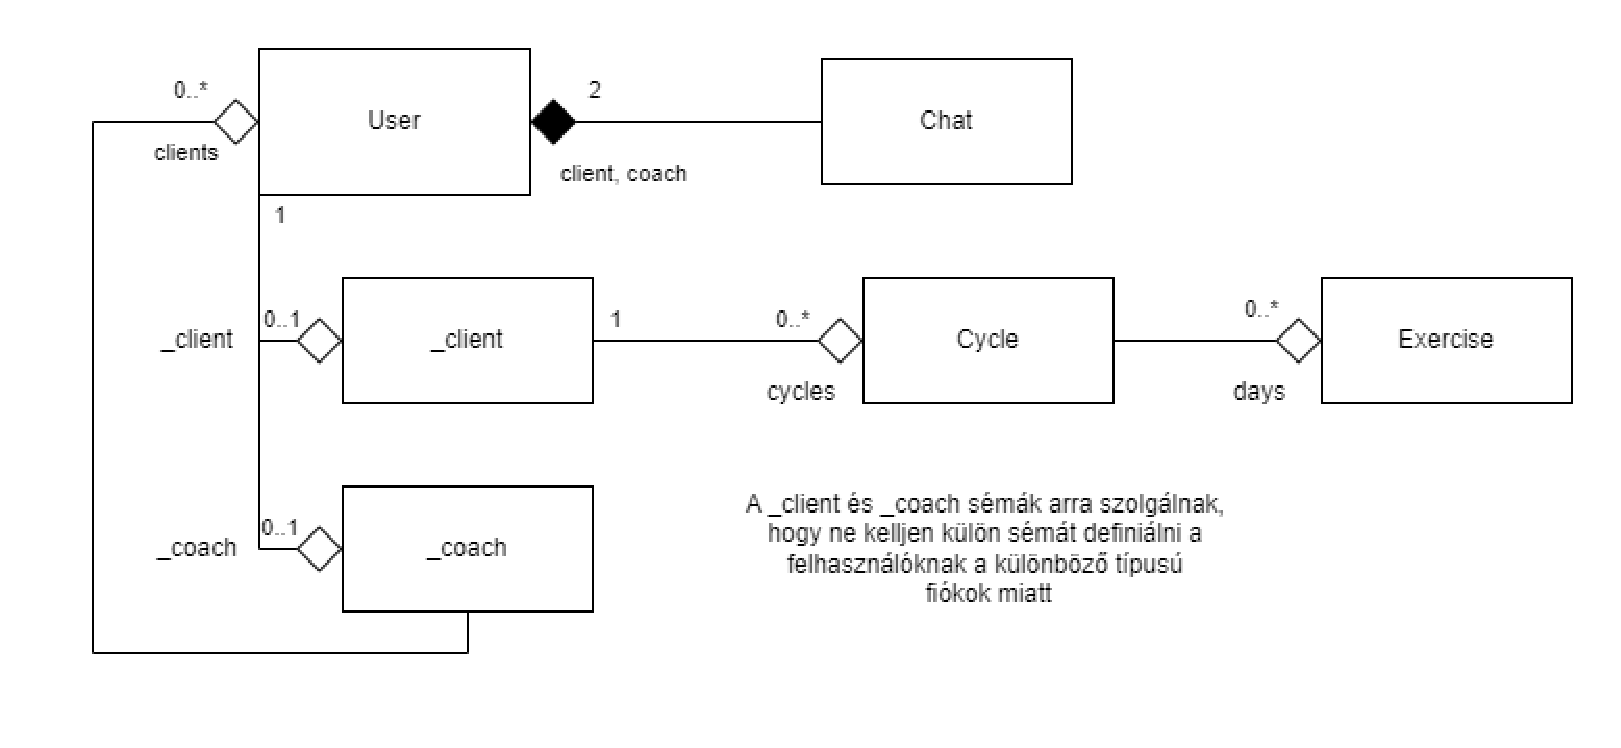
\includegraphics[width=1\linewidth]{model}
	\caption{Modellek (sémák) közötti kapcsolatok}
	\label{fig:model}
\end{figure}

Programomban a "server/schemas" útvonalon érhetőek el az ábrán látható sémák.

\subsection{View}

A view (nézet) felelős az alkalmazás felhasználói felületének megjelenítéséért és a felhasználói interakciók kezeléséért. Ide tartozik az UI elemek létrehozása, elrendezése és formázása, valamint az eseménykezelők hozzárendelése.

A kliensoldali nézetek megjelenítéséért és kezeléséért felelős React komponensek (.jsx kiterjesztésű fájlok, "client/src" útvonalon találhatók) a frontend alkalmazás részét képezik, és közvetlenül kommunikálnak a backenddel HTTP-n keresztül REST API kérések formájában

\subsection{Controller}

Programomban a controller rész a backenden, azaz a szerveroldalon található a "server/controllers" mappában. A Node.js környezetben a routerek és kontrollerek felelősek az útvonalak kezeléséért és az üzleti logika végrehajtásáért. Ezek a kontrollerek az HTTP kéréseket kezelik, és válaszolnak a megfelelő válaszokkal a kliens felé.

A következő alfejezetekben bemutatom a programban lévő kontrollereket, és ezek függvényeit. 

\subsubsection{Általános metódusok}

Ezek a metódusok minden modelhez tartoznak, alapvető adatbázis kezelő utasítások amelyeket a modellekre meghívhatunk.

\begin{itemize}
	\item Model.find(\{\}) - visszaadja az összes modellhez tartozó adatbázis objektumot
	\item Model.find(\{...searchparams\}) - visszaadja a legelső, paraméterekre illeszkedő adatbázis objektumot
	\item Model.save() - elmenti az adatbázisban az adott objektumot
	\item Model.updateOne(\{...searchparams\}, \{...changedattributes\}) - megkeresi a legelső illeszkedő objektumot, majd frissíti a megadott információkkal
	\item Model.deleteOne(\{...serachparams\}) - megkeresi a legelső illeszkedő objektumot és törli az adatbázisból
\end{itemize}

A tobábbiakban A req, res paraméterek a \emph{Request} (kérés) és \emph{Response} (válasz). Mivel a kliensoldal és szerveroldal REST API kérésekkel kommunikál egymással, minden szükséges információ a műveletek végrehajtásához a \emph{Request} paraméterben lesz tárolva JSON formátumban. A \emph{Response} paraméter tartalma pedig visszakerül 

\subsubsection{CycleController}

\begin{figure}[H]
	\centering
	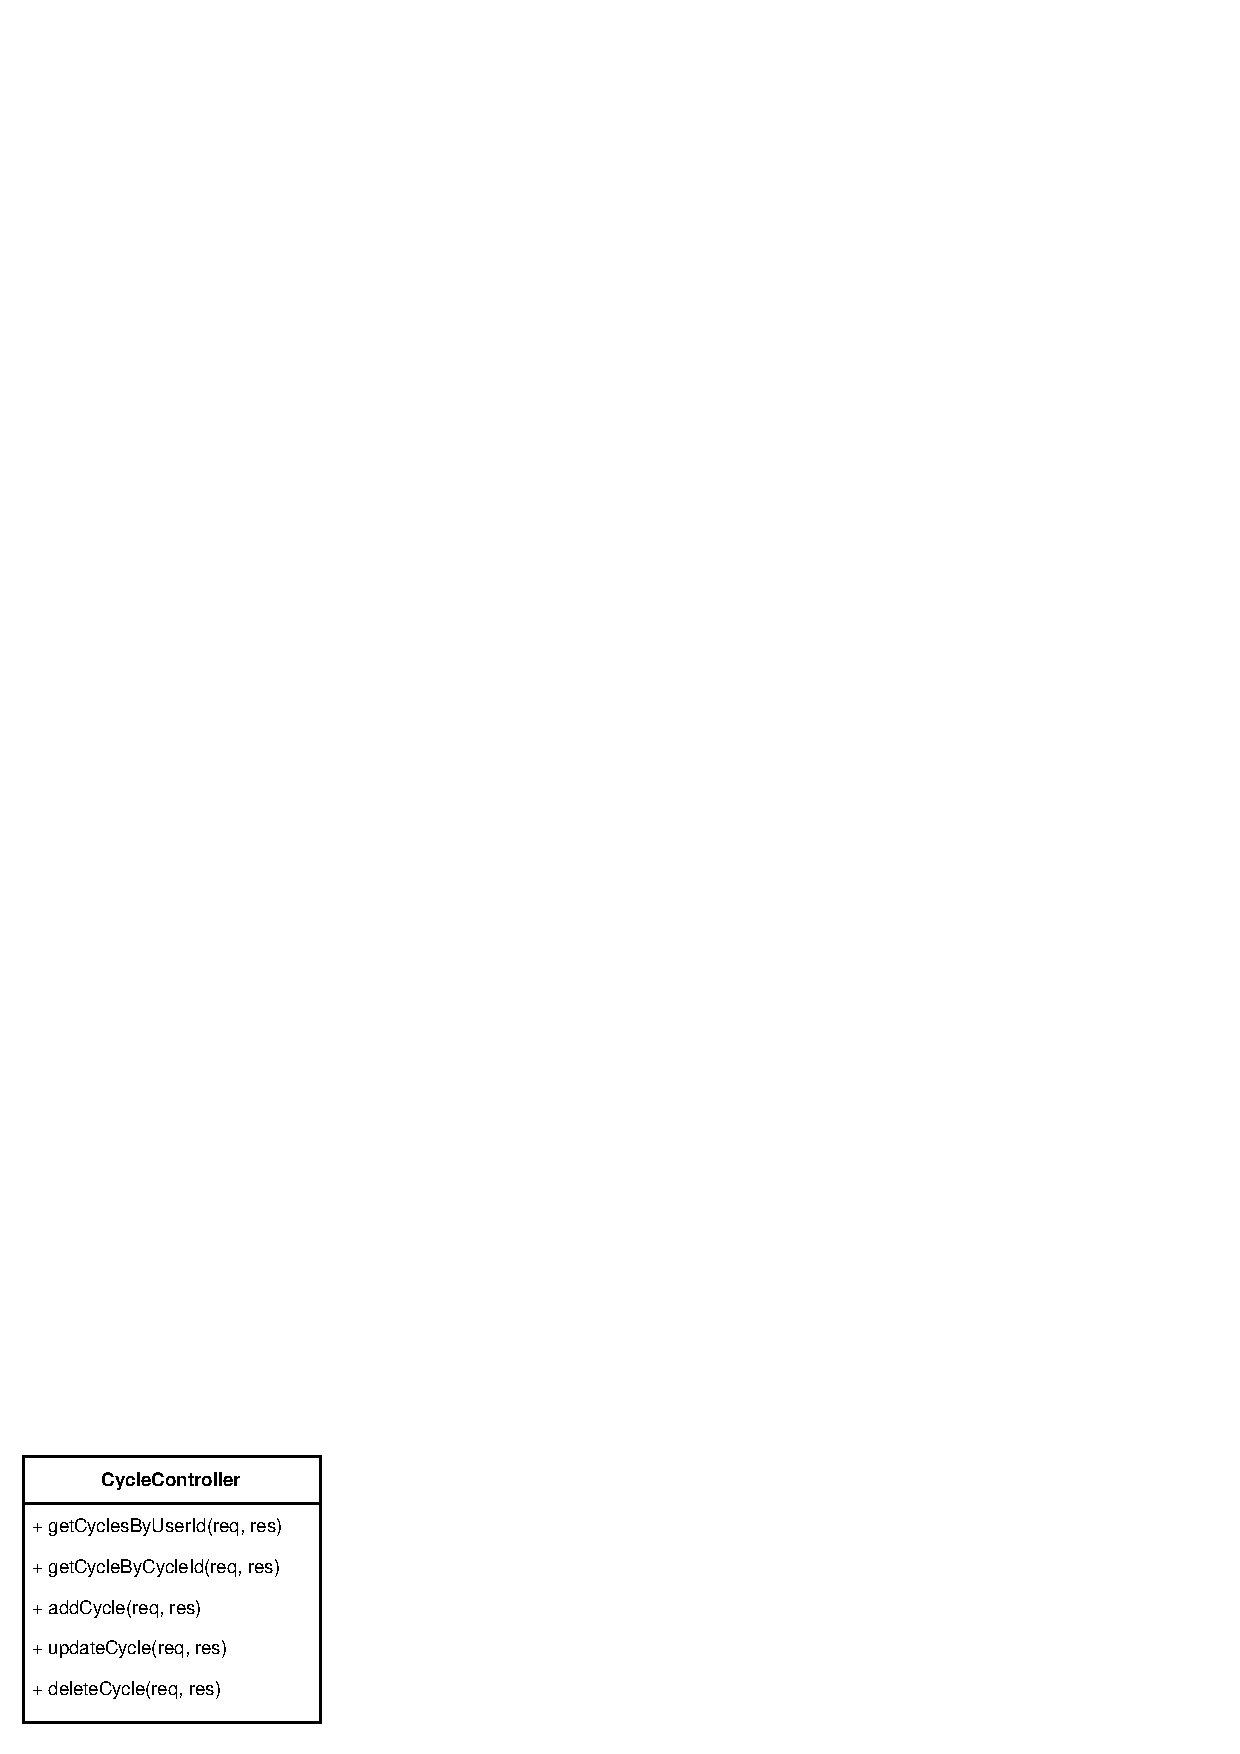
\includegraphics[width=0.4\linewidth]{cyclecontroller}
	\caption{CycleController osztály}
	\label{fig:cyclecontroller}
\end{figure}

A \ref{fig:cyclecontroller} ábrán láthatóak a CycleController osztály metódusai.

\begin{description}
	\item[getCyclesByUserId(req, res):] Visszaadja egy adott felhasználó hoz (ID szerint) tartozó összes ciklus objektumot
	\item[getCycleByCycleId(req, res):] Visszaad egy ciklus objektumot ID alapján
	\item[addCycle(req, res):] A kérésben található JSON-ban tárolt információ alapján létrehoz egy ciklus adatbázis objektumot az adott felhasználóhoz rendelve
	\item[updateCycle(req, res):] Ciklus ID alapján megkeresi a kért objektumot az adatbázisban, és a kérésben JSON-ban tárolt információkra cseréli ki az objektum tartalmát
	\item[deleteCycle(req, res):] Ciklus ID alapján törli a talált objektumot az adatbázisból  
\end{description}

Ha véletlenül egy olyan adatbázis objektumra hívunk meg egy metódust, amelyre nincsen értelmezve, a szerver hibaüzenettel fog visszatérni. Például ha egy edző típusú felhasználóhoz szeretnénk egy új ciklust hozzáadni, a program le fogja kezelni az esetet és hibával tér vissza. 

Ilyen fajta hibakezeléssel mindegyik kontroller rendelkezik, middleware-ként vannak definiálva ezek az ellenőrző és hibakezelő függvények.

\subsubsection{UserController}

\begin{figure}[H]
	\centering
	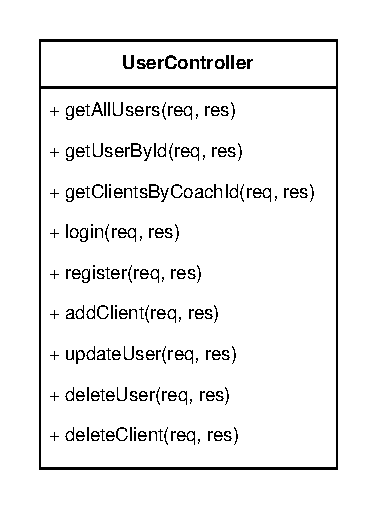
\includegraphics[width=0.4\linewidth]{usercontroller}
	\caption{UserController osztály}
	\label{fig:usercontroller}
\end{figure}

A \ref{fig:usercontroller} ábrán láthatóak a UserController osztályhoz tartozó függvények.

\begin{description}
	\item[getClientsByCoachId(req, res):] Edző objektumnak adja vissza az összes hozzárendelt kliens objektumot
	\item[login(req, res):] Bejelentkezést kezeli, sikeres hitelesítés után egy aláírt JWT tokent küld vissza a kliensnek
	\item[register(req, res):] Sikeres regisztráció után egy aláírt JWT tokent küld vissza, illetve kezeli az edzőhöz való ID alapú hozzárendelést is
	\item[addClient(req, res):] Kliens objektumok edzőhöz való rendelésére szolgál
	\item[deleteUser(req, res):] Töröl egy felhasználót az adatbázisból, ha kliens típusú akkor a hozzá tartozó ciklusokat is törli
	\item[deleteClient(req, res):] Megszüntet egy kliens-edző hozzárendelést
\end{description}

A getAllUsers, getUserById, updateUser metódusokhoz nem szükséges külön magyarázat, ezek a függvények minden fajta User objektumra használhatóak.

\subsubsection{ChatController}

\begin{figure}[H]
	\centering
	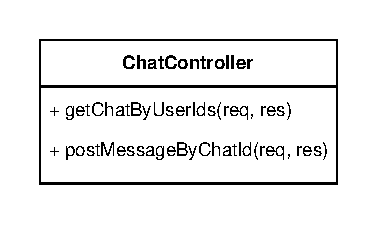
\includegraphics[width=0.4\linewidth]{chatcontroller}
	\caption{ChatController osztály}
	\label{fig:chatcontroller}
\end{figure}

A \ref{fig:chatcontroller} ábrán látható a ChatController osztály metódusai.

\begin{description}
	\item[getChatByUserIds(req, res):] Egy kliens és egy edző közötti chatet keresi meg, a két felhaszáló azonosítójából
	\item[postMessageByChatId(req, res):] Üzenet elküldésére szolgál egy chatben
\end{description}


\subsection{Router}

Ebben az alfejezetben a \textbf{Router} REST API útvonalait fogom felsorolni és leírni a hozzá tartozó kontroller hívást. A \emph{":param"} szöveg mindig egy paramétert jelent az útvonalakban.

\subsubsection{\underline{GET végpontok}}

\begin{description}
	\item[/users] - UserController.getAllUsers
	\item[/users/:id] - UserController.getUserById 
	\item[/users/:id/cycles] - CycleController.getCyclesByUserId
	\item[/users/:id/cycles/:cycleid] - CycleController.getCycleByCycleId
	\item[/users/:id/clients] - UserController.getClientsByCoachId
	\item[/chat/:clientId/:coachId] - ChatController.getChatByUserIds
\end{description}

\subsubsection*{\underline{POST végpontok}}

\begin{description}
	\item[/auth/login] - UserController.login
	\item[/auth/register] - UserController.register
	\item[/users/:id/cycles] -  CycleController.addCycle
	\item[/users/:id/clients] - UserController.addClient
	\item[/chat/:chatId] - ChatController.postMessageByChatId
\end{description}

\subsubsection{\underline{PATCH végpontok}}

\begin{description}
	\item[/users/:id/cycles/:cycleid] - CycleController.updateCycle
	\item[/users/:id] - UserController.updateUser
\end{description}

\subsubsection{\underline{DELETE végpontok}}

\begin{description}
	\item[/users/:id] - UserController.deleteUser
	\item[/users/:id/cycles/:cycleid] - CycleController.deleteCycle
	\item[/users/:id/clients/:clientid] - UserController.deleteClient
\end{description}


\subsection{Middlerwarek}

\begin{itemize}
	\item authMiddleware
	\begin{itemize}
		\item authenticateToken - Ez a függvény felel a JWT tokenek hitelesítéséért, ellenőrzi hogy az aláírás és lejárati időbélyeg valid-e
	\end{itemize}
	\item userTypeMiddleware
	\begin{itemize}
		\item userTypeClient - Ellenőrzi, hogy a kérést küldő felhasználó létezik-e és valóban kliens típusú
		\item userTypeCoach - Ugyanez, edző felhasználóra
		\item userTypeAdmin - Ugyanez, adminisztrátor felhasználóra
		\item isClientIdValid - Ellenőrzi, hogy a kapott ID hivatkozik-e egy kliens objektumra
		\item isCoachIdValid - Ugyanez, edző felhasználóra
	\end{itemize}
\end{itemize}



\begin{landscape}
\section{Adatbázis}
\label{ch:adatbazis}
	\begin{figure}[H]
		\centering
		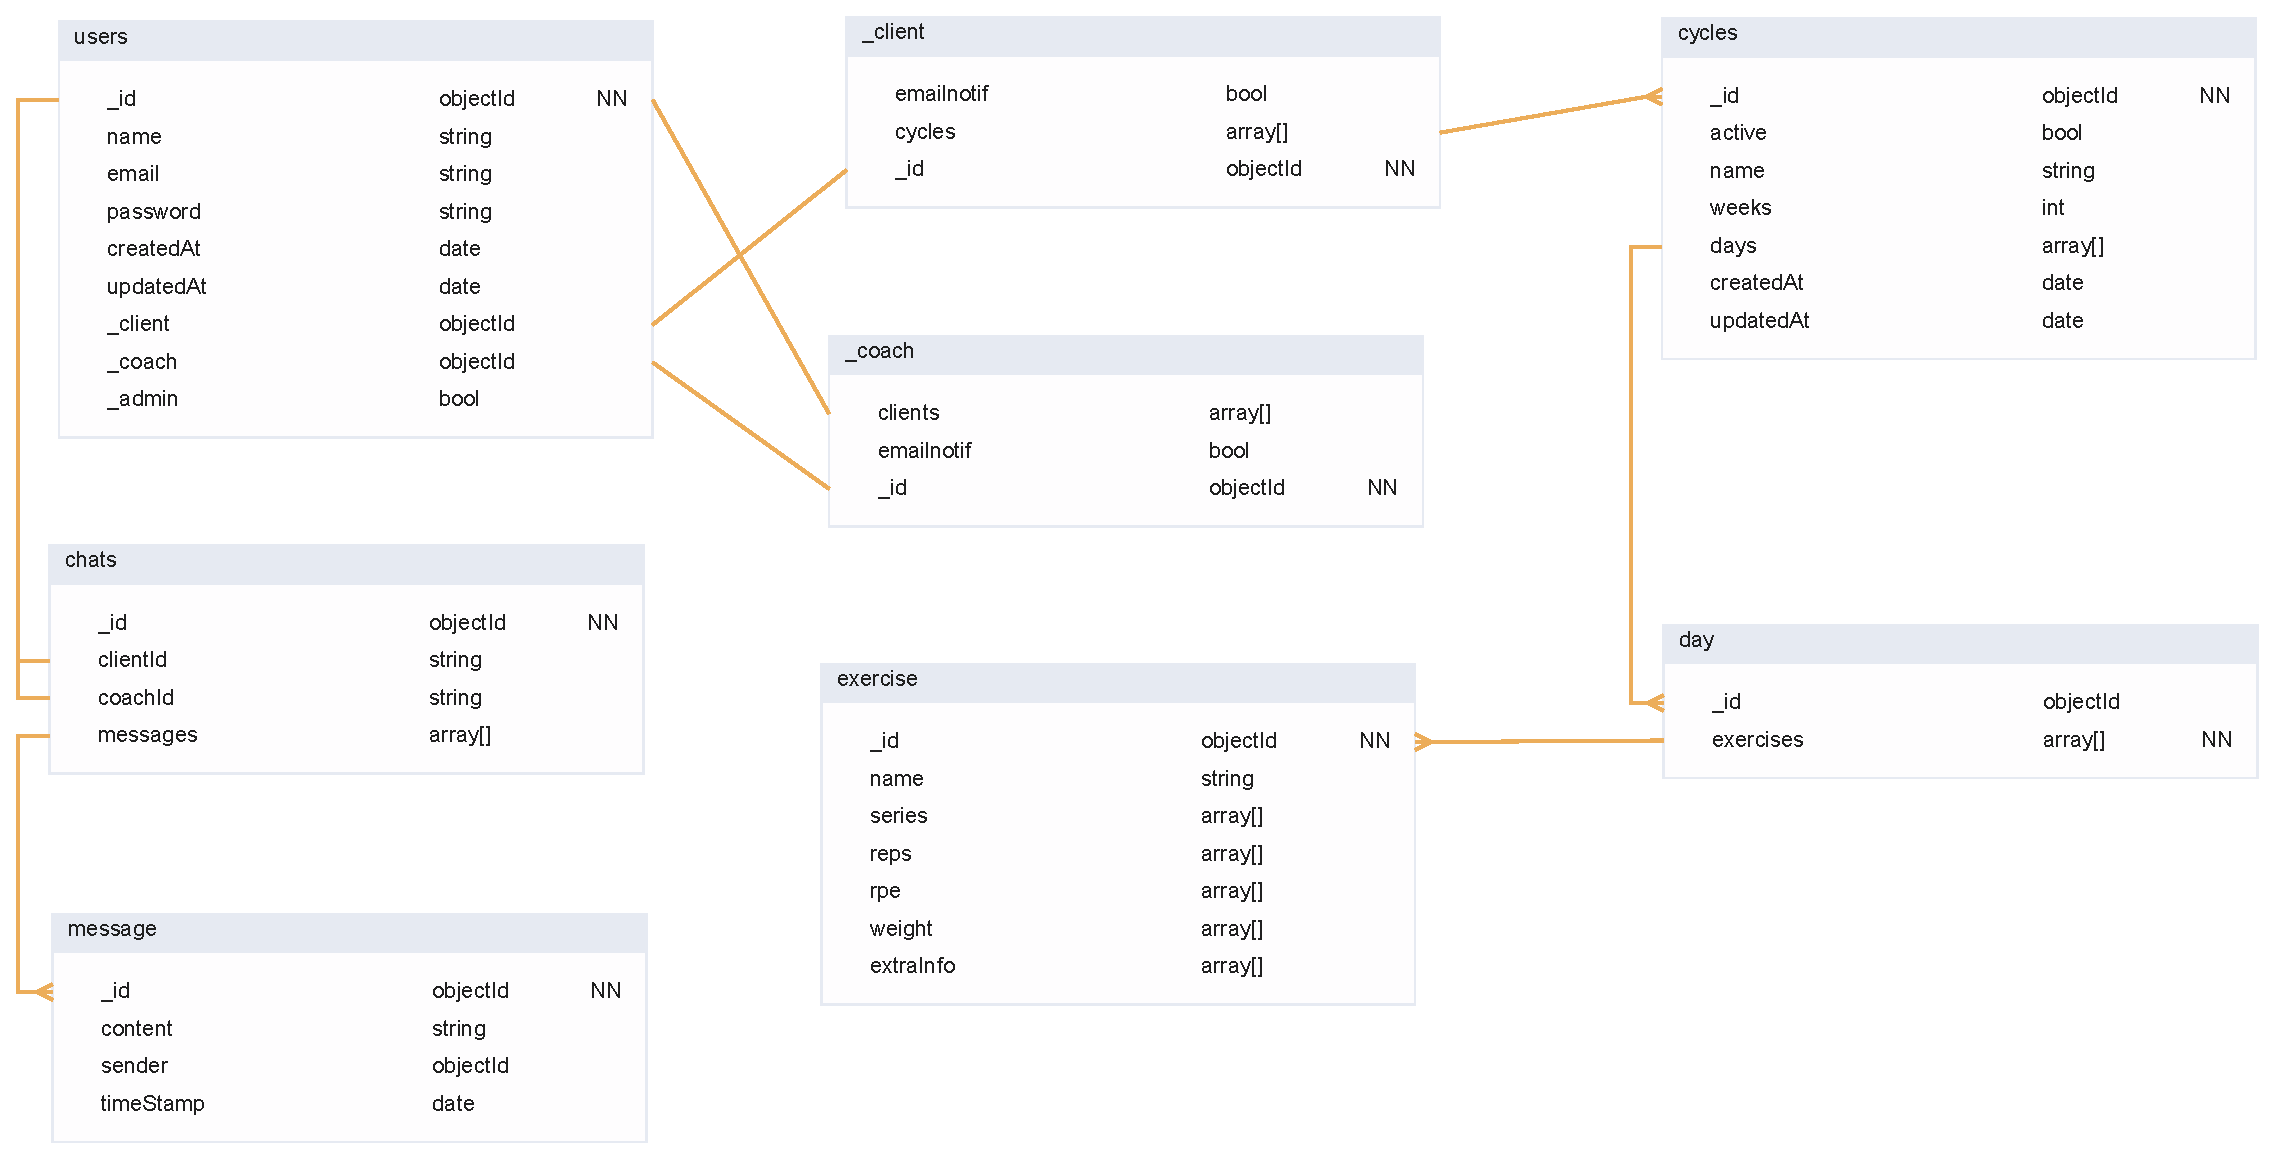
\includegraphics[width=1\linewidth]{adatbazis}
		\caption{Adatbázis (készült a MongoModeler \cite{mongomodeler} program segítségével)}
		\label{fig:adatbazis}
	\end{figure}
\end{landscape}

\subsection{Gyűjtemények}

\begin{description}
	\item[Users:] Ez a gyűjtemény felelős a felhasználók információjának tárolásáról. Név, email cím, jelszó és időbélyegek tárolásán kívül a \_client, \_coach és \_admin attribútumokban kerül tárolásra a fiók típusa. A \_client és \_coach mezők hivatkozhatnak egy objektumra, amelyben extra adatokat tárolunk az ilyen típusú felhasználókról.
	\item[\_client:] Ez egy segéd gyűjtemény a Users-en belül, tárolja az email értesítések állapotát és a kliens ciklusait, amely egy ObjectId-kat tartalmazó tömb.
	\item[\_coach:] Ez szintén egy segéd gyűjtemény, itt az edzőknek is az email értesítés állapotát és a klienseket tároljuk egy tömbben, mint ObjectId-k.
	\item[Chats:] Itt tárolódnak a felhasználók közötti beszélgetések. A gyűjteménynek a clientId és coachId a kulcsa együttesen. A messages tömbben tárolódnak az üzenetek, mint objektumok.
	\item[Message:] Ebben a segéd gyűjteményben tároljuk az egyes üzeneteket, tartalommal és egyéb információkkal. 
	\item[Cycles:] Minden edzéstervvel kapcsolatos adatot ebben a gyűjteményben tároljuk. A days tömb ObjectId-kat tartalmaz, ilyen módon össze van kapcsolva a \textbf{day} segéd gyűjteménnyel.
	\item[day:] Itt csupán egy tömbben tároljuk az adott indexű naphoz tartozó gyakorlatokat, amelyeket a \textbf{exercise} segédgyűjtemény tartalmaz.
	\item[exercise:] A gyakorlatok összes adata itt található. A gyakorlat nevén kívül minden adat tömbben tárolódik (amelynek mérete azonos az edzéstervben lévő hetek számával), így szimulálva a heteket az edzéstervben.
\end{description}

\subsection{Adatbázis motor}

Alkalmazásomban az adatbázis megvalósításához MongoDB-t \cite{mongodb} használtam. Ez egy NoSQL adatbázis, így működésben kissé eltér egy általános SQL adatbázismotortól, kevesebb megszorítással rendelkezik. Szakdolgozatom írása során próbáltam ennek a technológiának előnyeit kihasználni, miközben betartva a különböző konvenciókat és tervezési módszereket amelyekkel tanulmányaim során találkoztam. 


\section{Felhasználói felület terve}

\subsection{Kezdőlap}
\begin{figure}[H]
	\centering
\fbox{	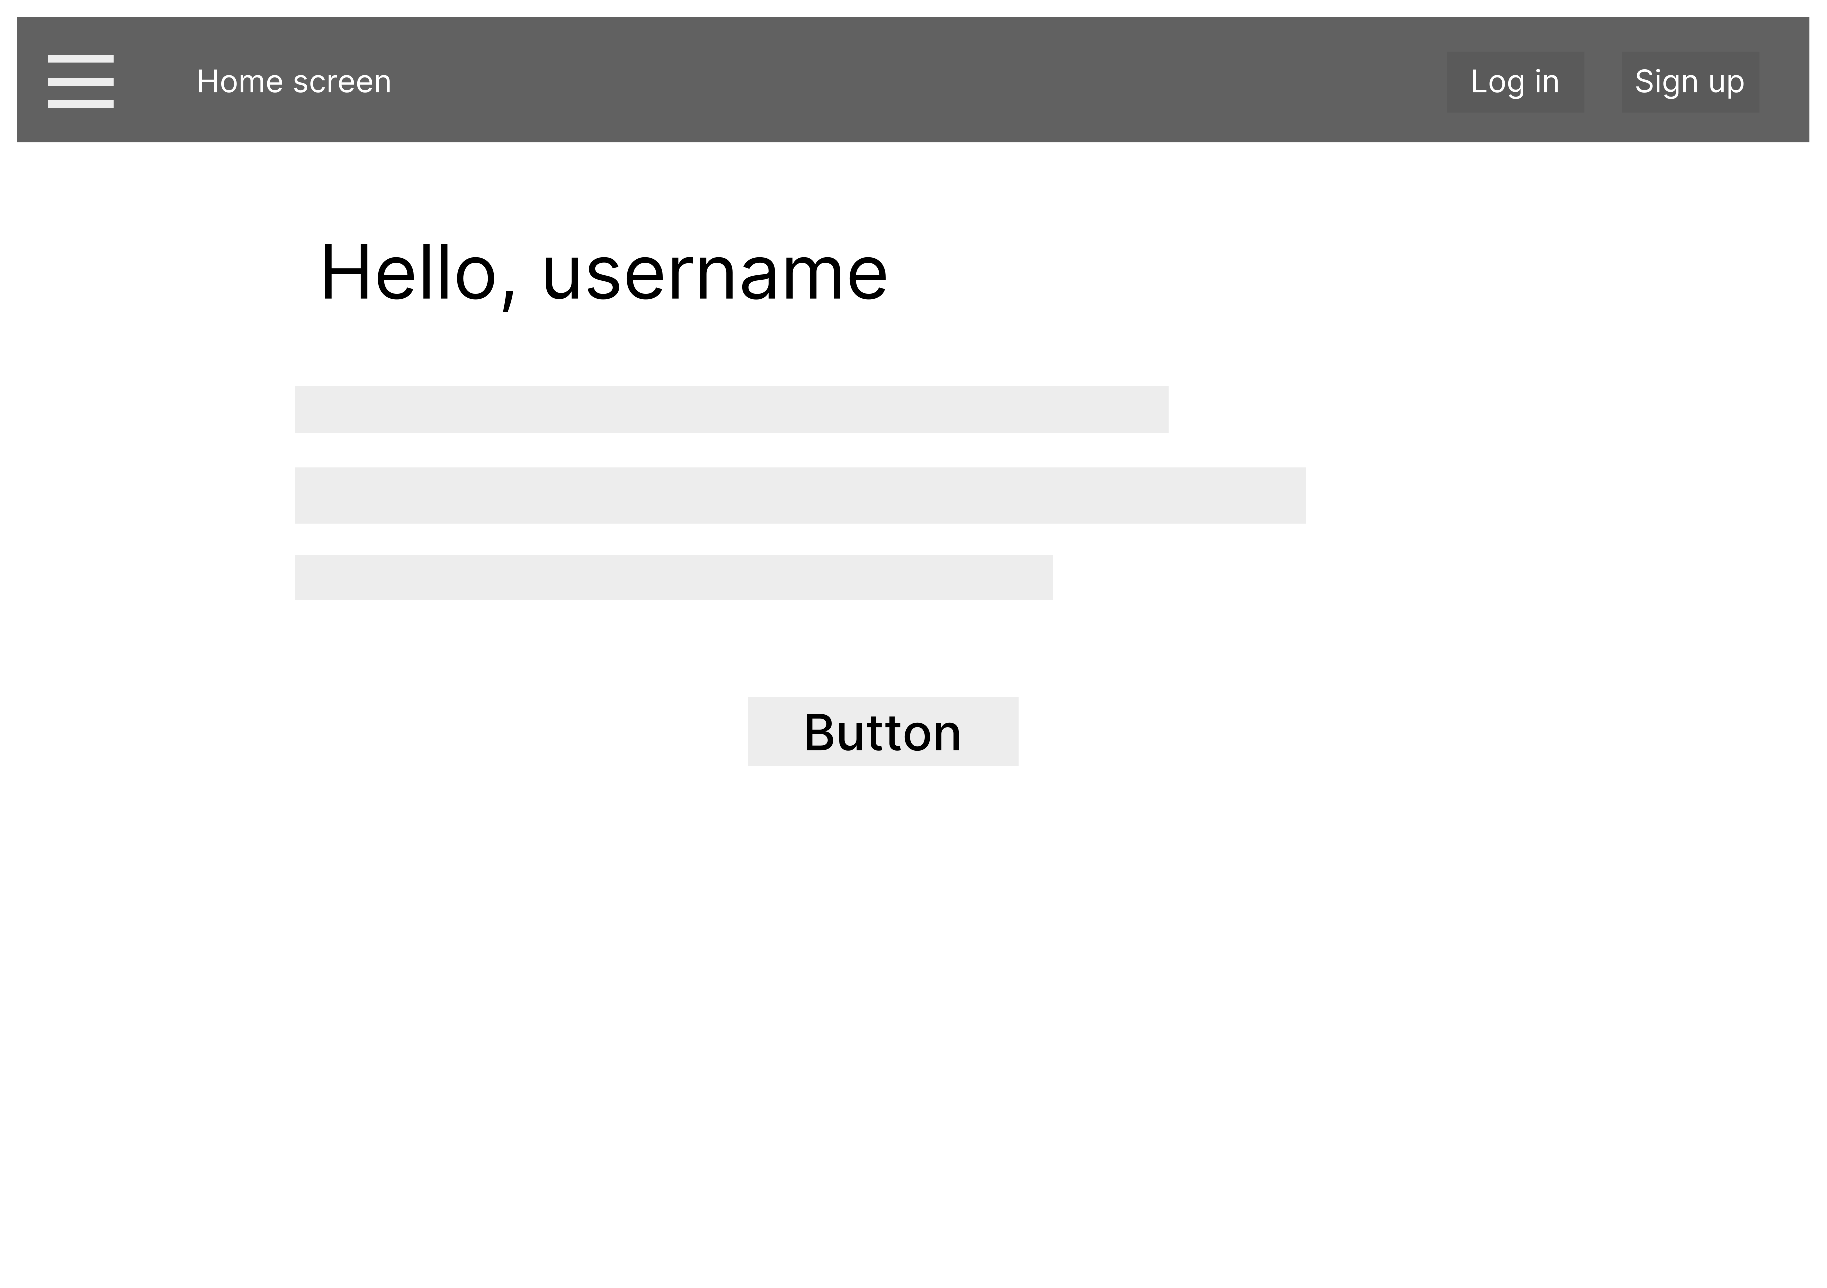
\includegraphics[width=0.8\linewidth]{homepage}
}	\caption{Kezdőlap drótváza}
	\label{fig:homepage}
\end{figure}

\subsection{Bejelentkezés oldal}
\begin{figure}[H]
	\centering
\fbox{	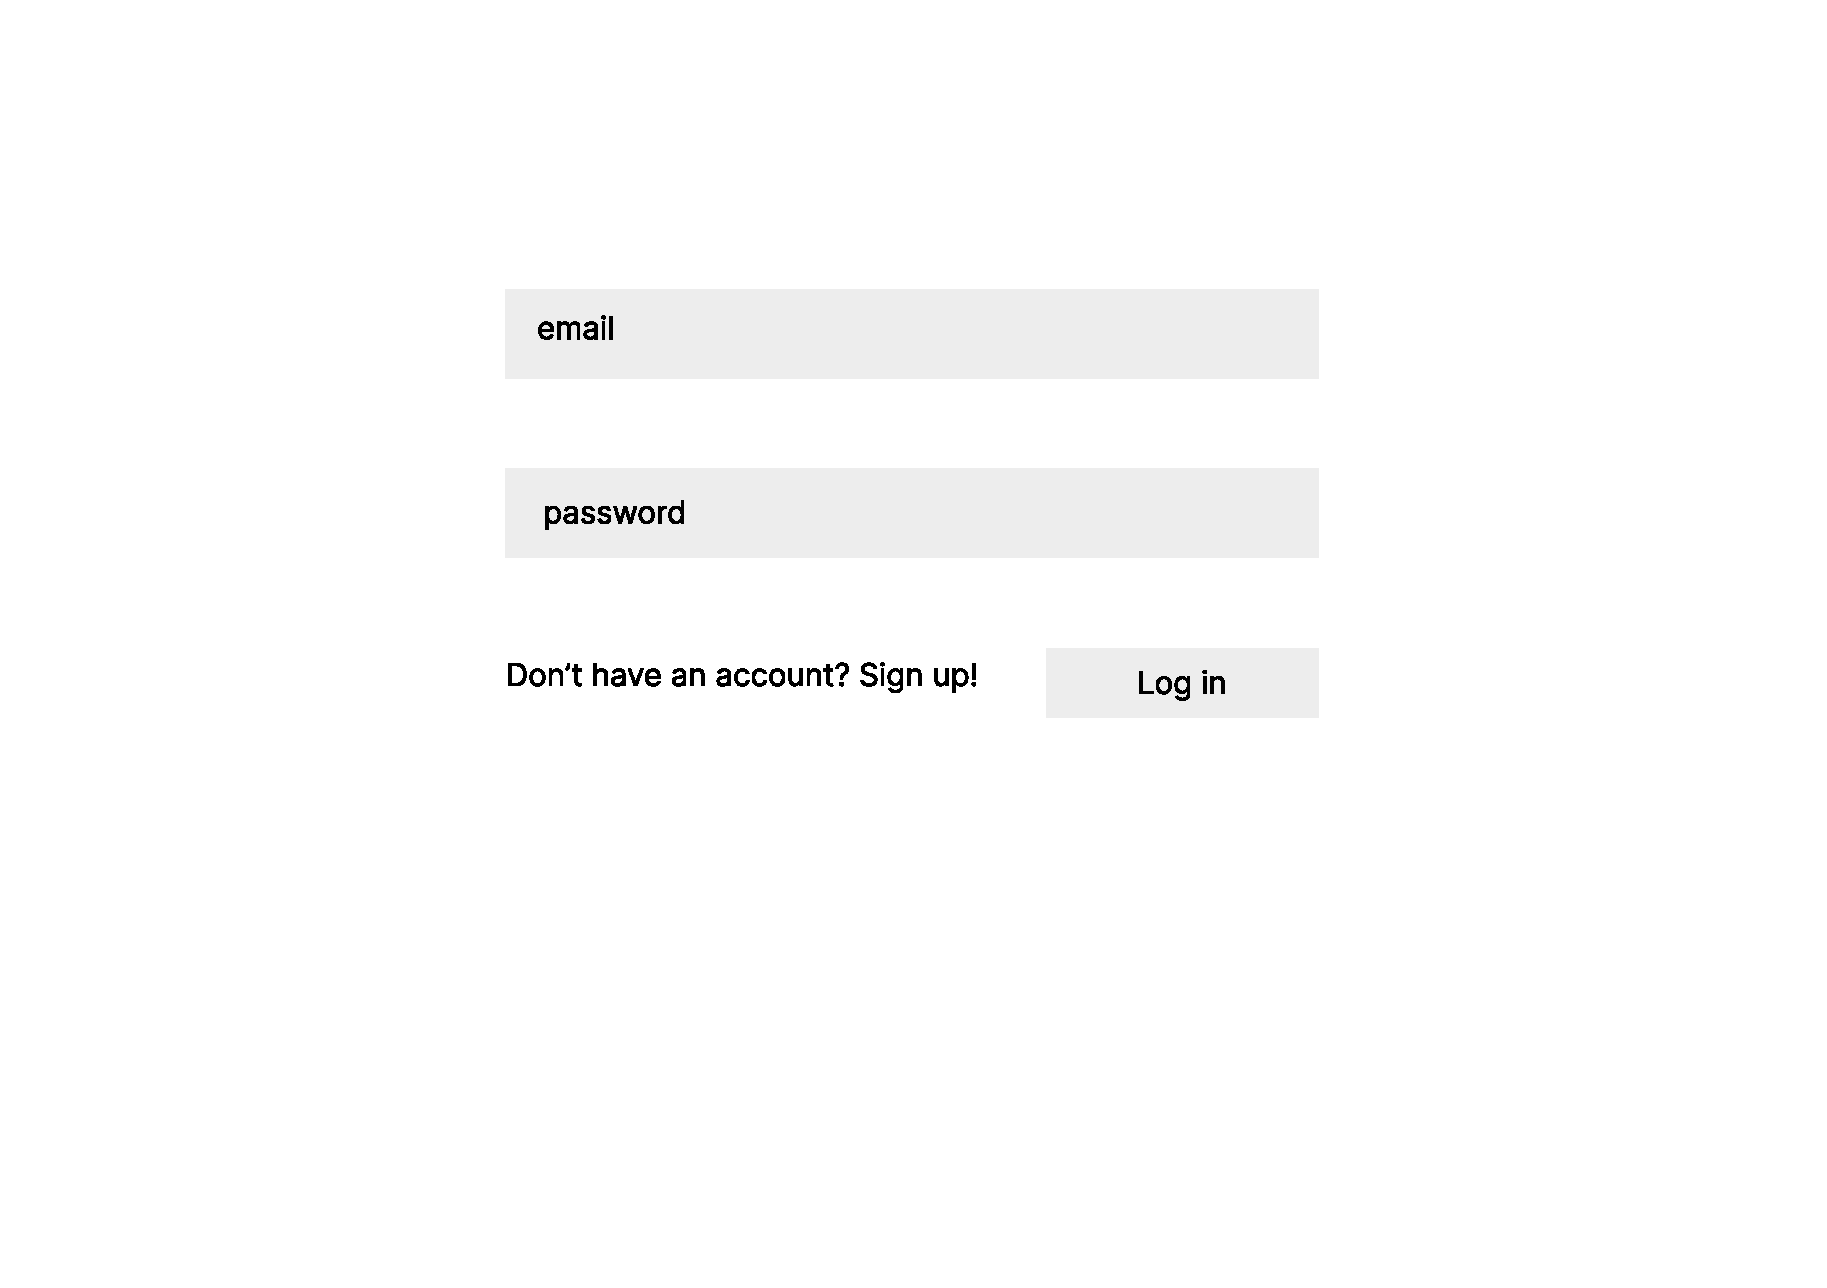
\includegraphics[width=0.8\linewidth]{loginscreen}
}	\caption{Bejelentkezési oldal drótváza}
	\label{fig:loginscreen}
\end{figure}

\subsection{Regisztrációs oldal}
\begin{figure}[H]
	\centering
\fbox{	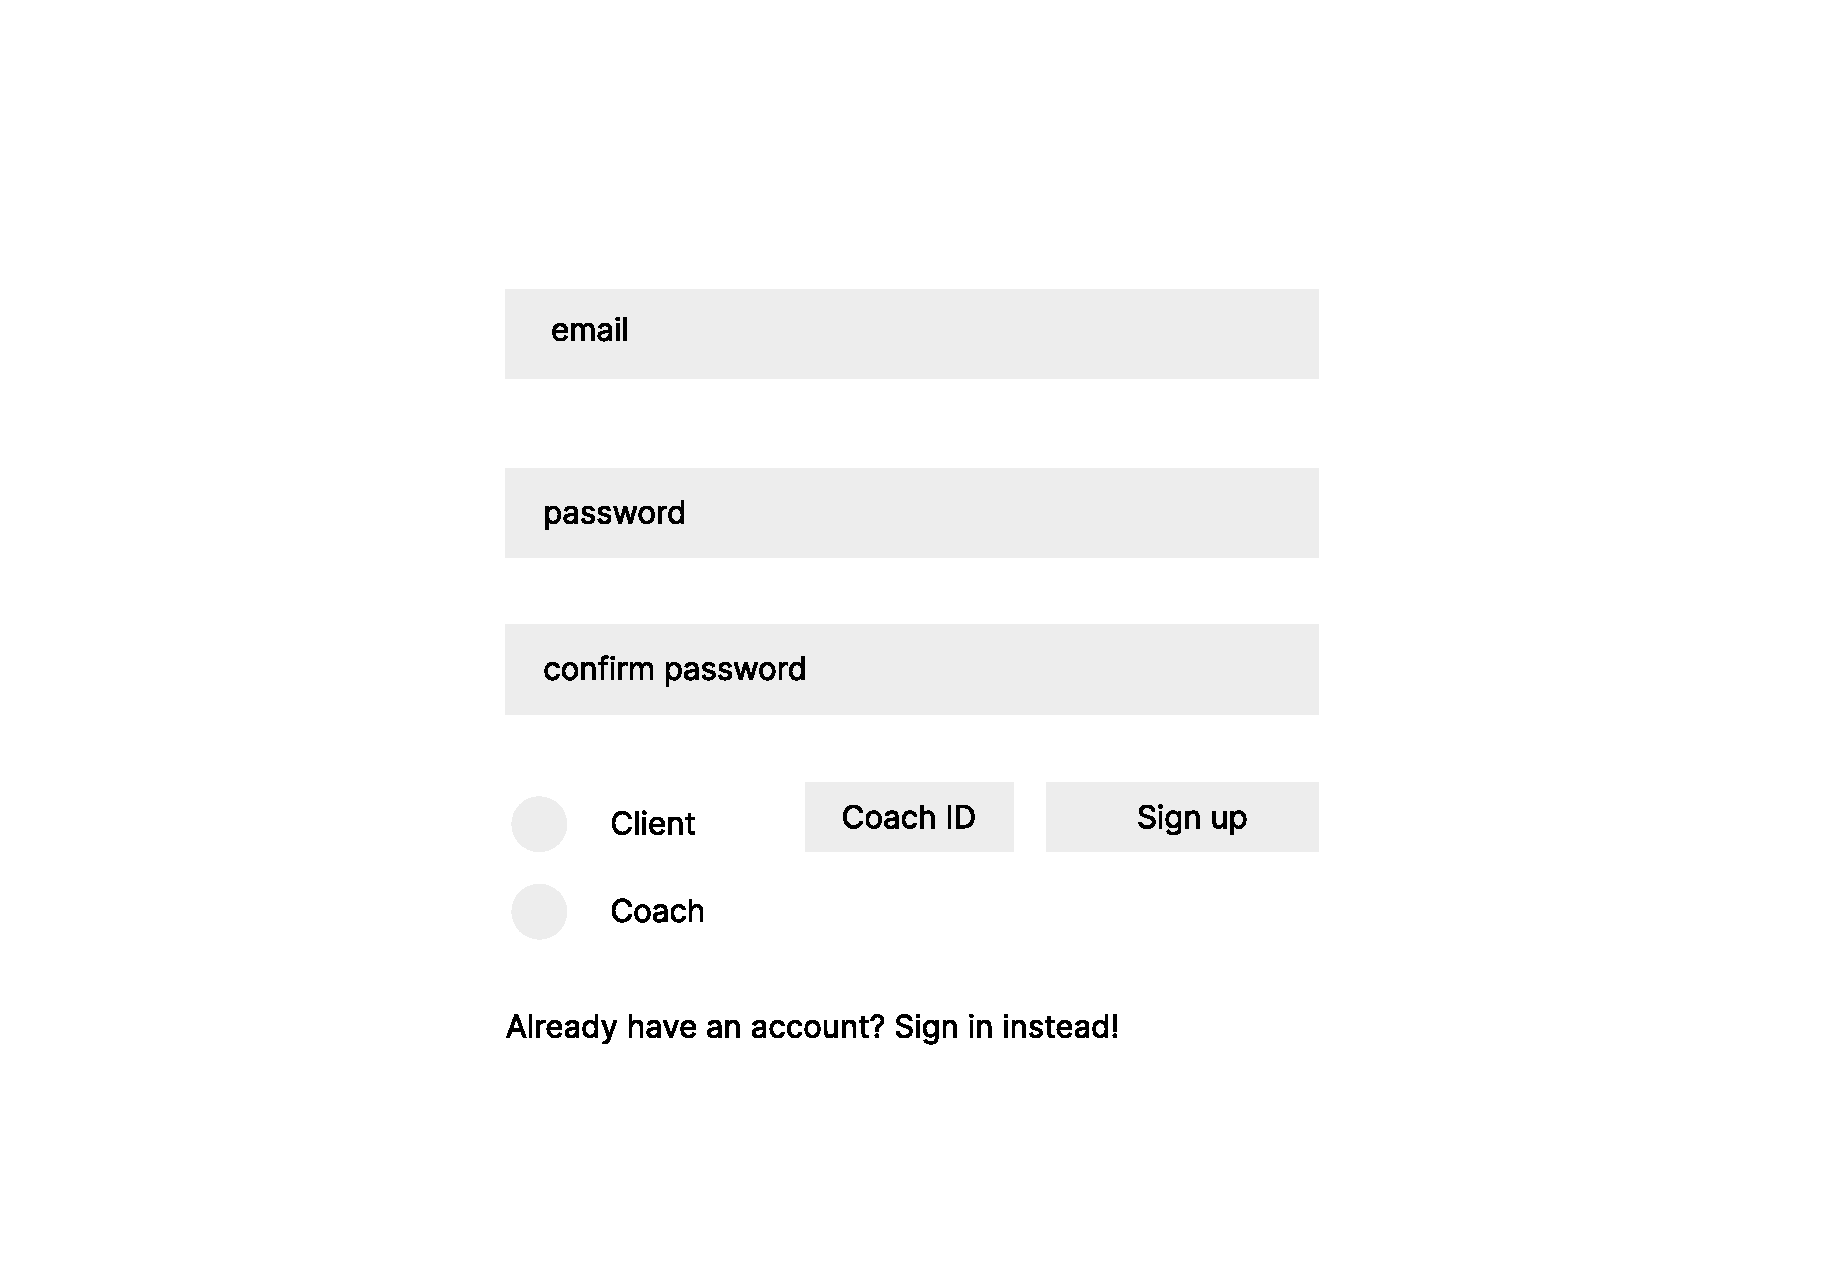
\includegraphics[width=0.8\linewidth]{signupscreen}
}	\caption{Regisztráció oldal drótváza}
	\label{fig:signupscreen}
\end{figure}

\subsection{Navigációs menü}
\begin{figure}[H]
	\centering
\fbox{	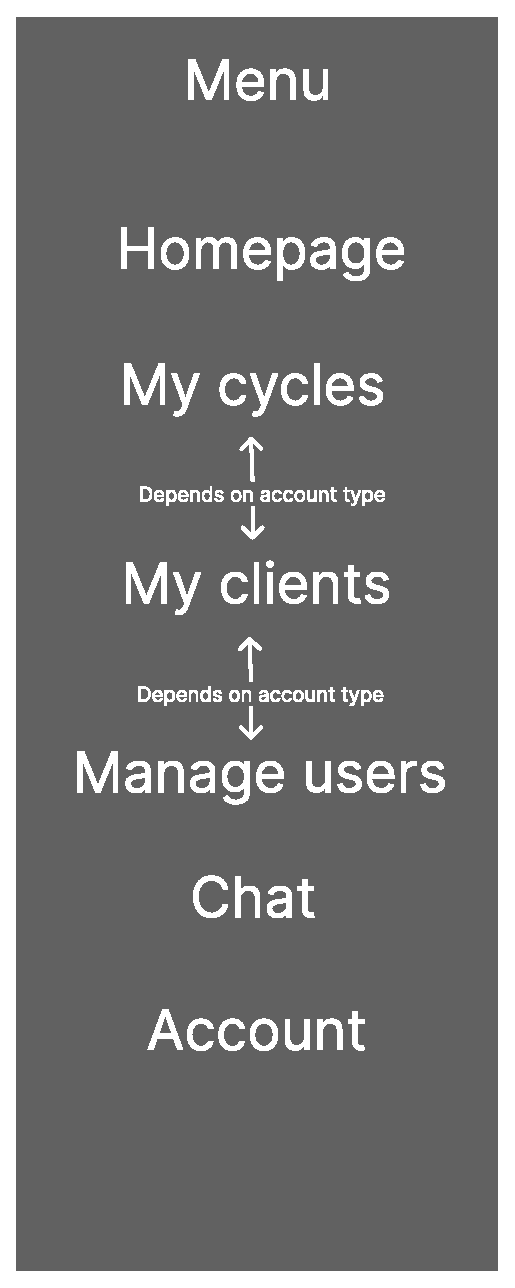
\includegraphics[width=0.25\linewidth]{menu}
}	\caption{Navigációs menü drótváza}
	\label{fig:menu}
\end{figure}

\subsection{Ciklusok listázó oldala}
\begin{figure}[H]
	\centering
\fbox{	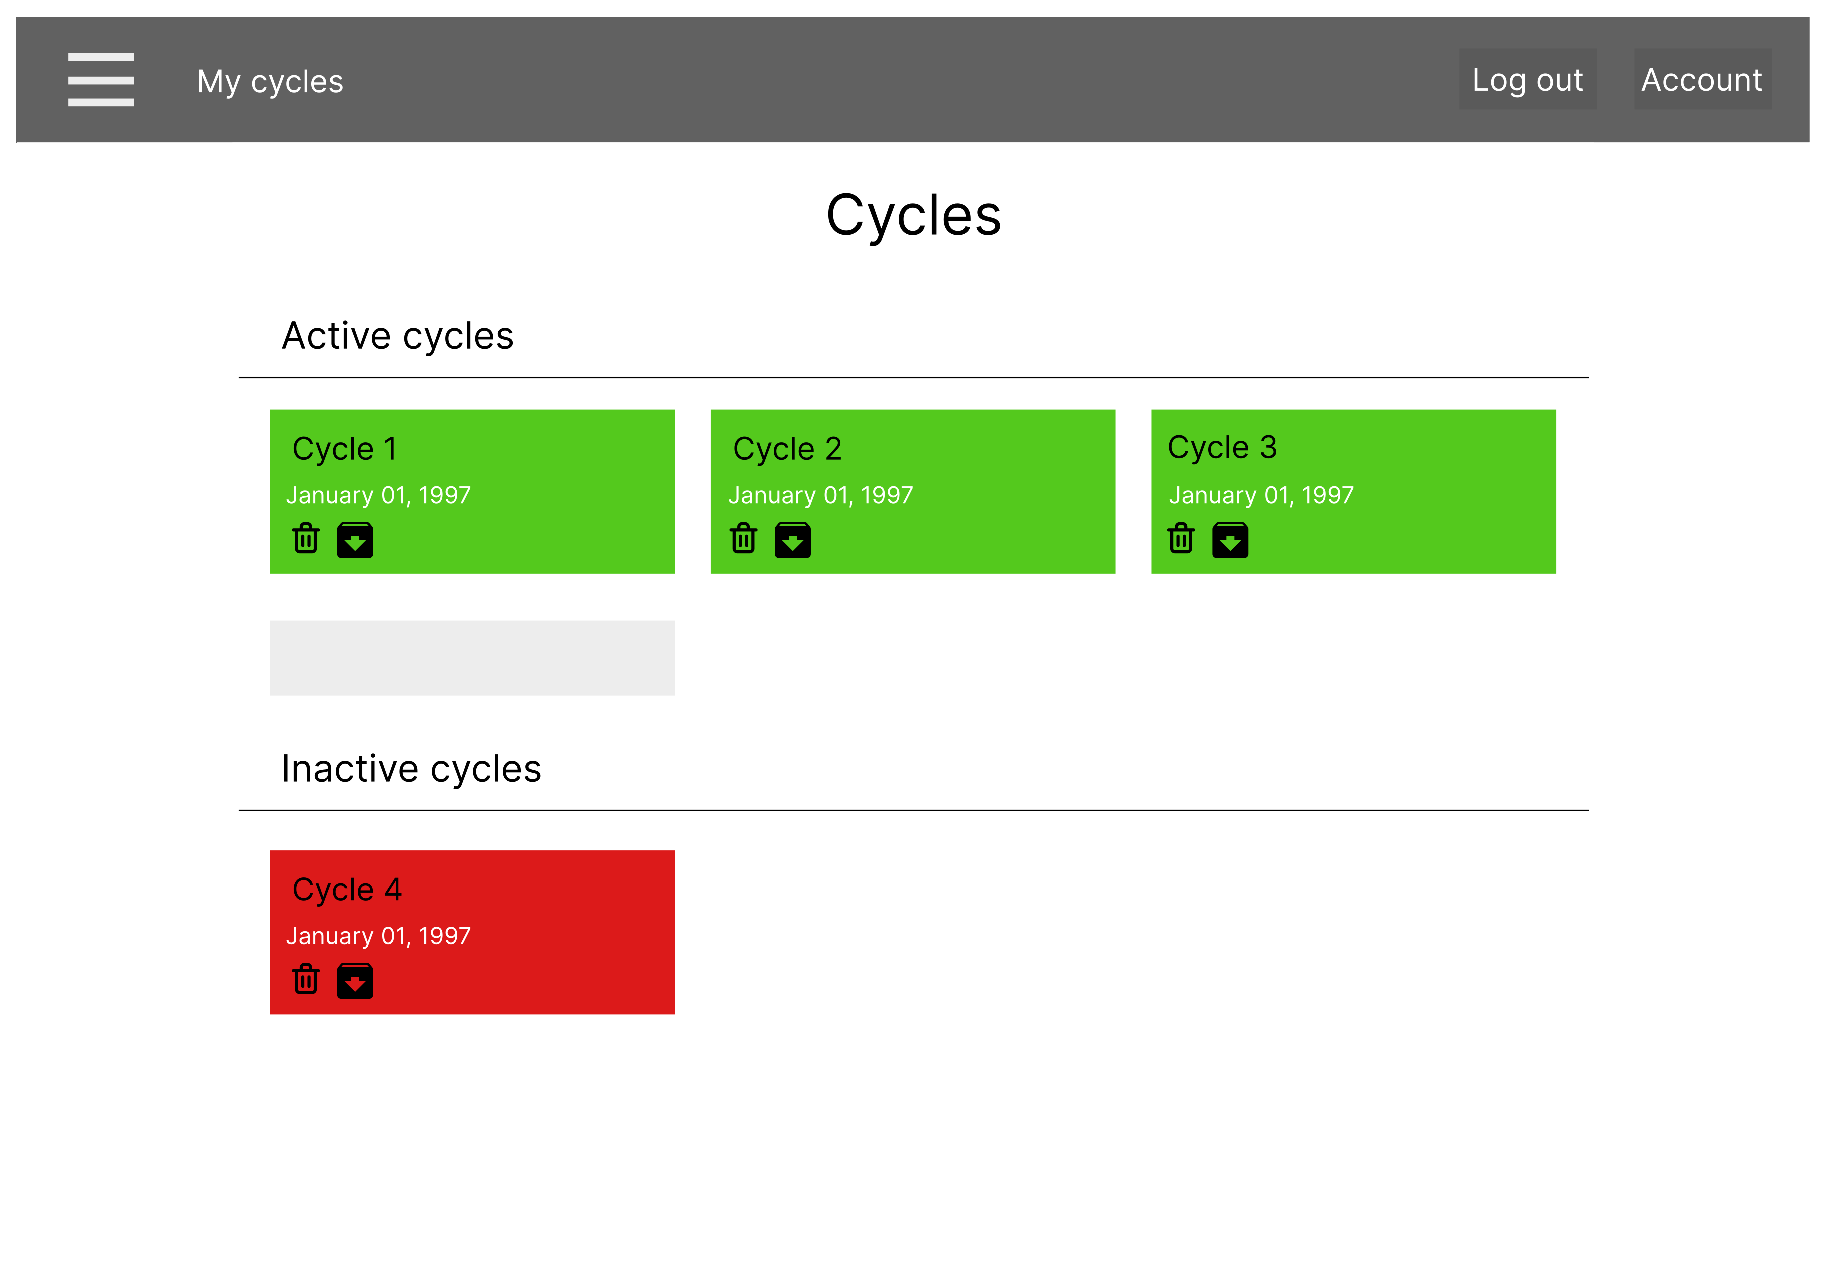
\includegraphics[width=0.8\linewidth]{cyclespage}
}	\caption{Ciklusok listázó oldal drótváza}
	\label{fig:cyclespage}
\end{figure}

\subsection{Edzésterv oldal}
\begin{figure}[H]
	\centering
\fbox{	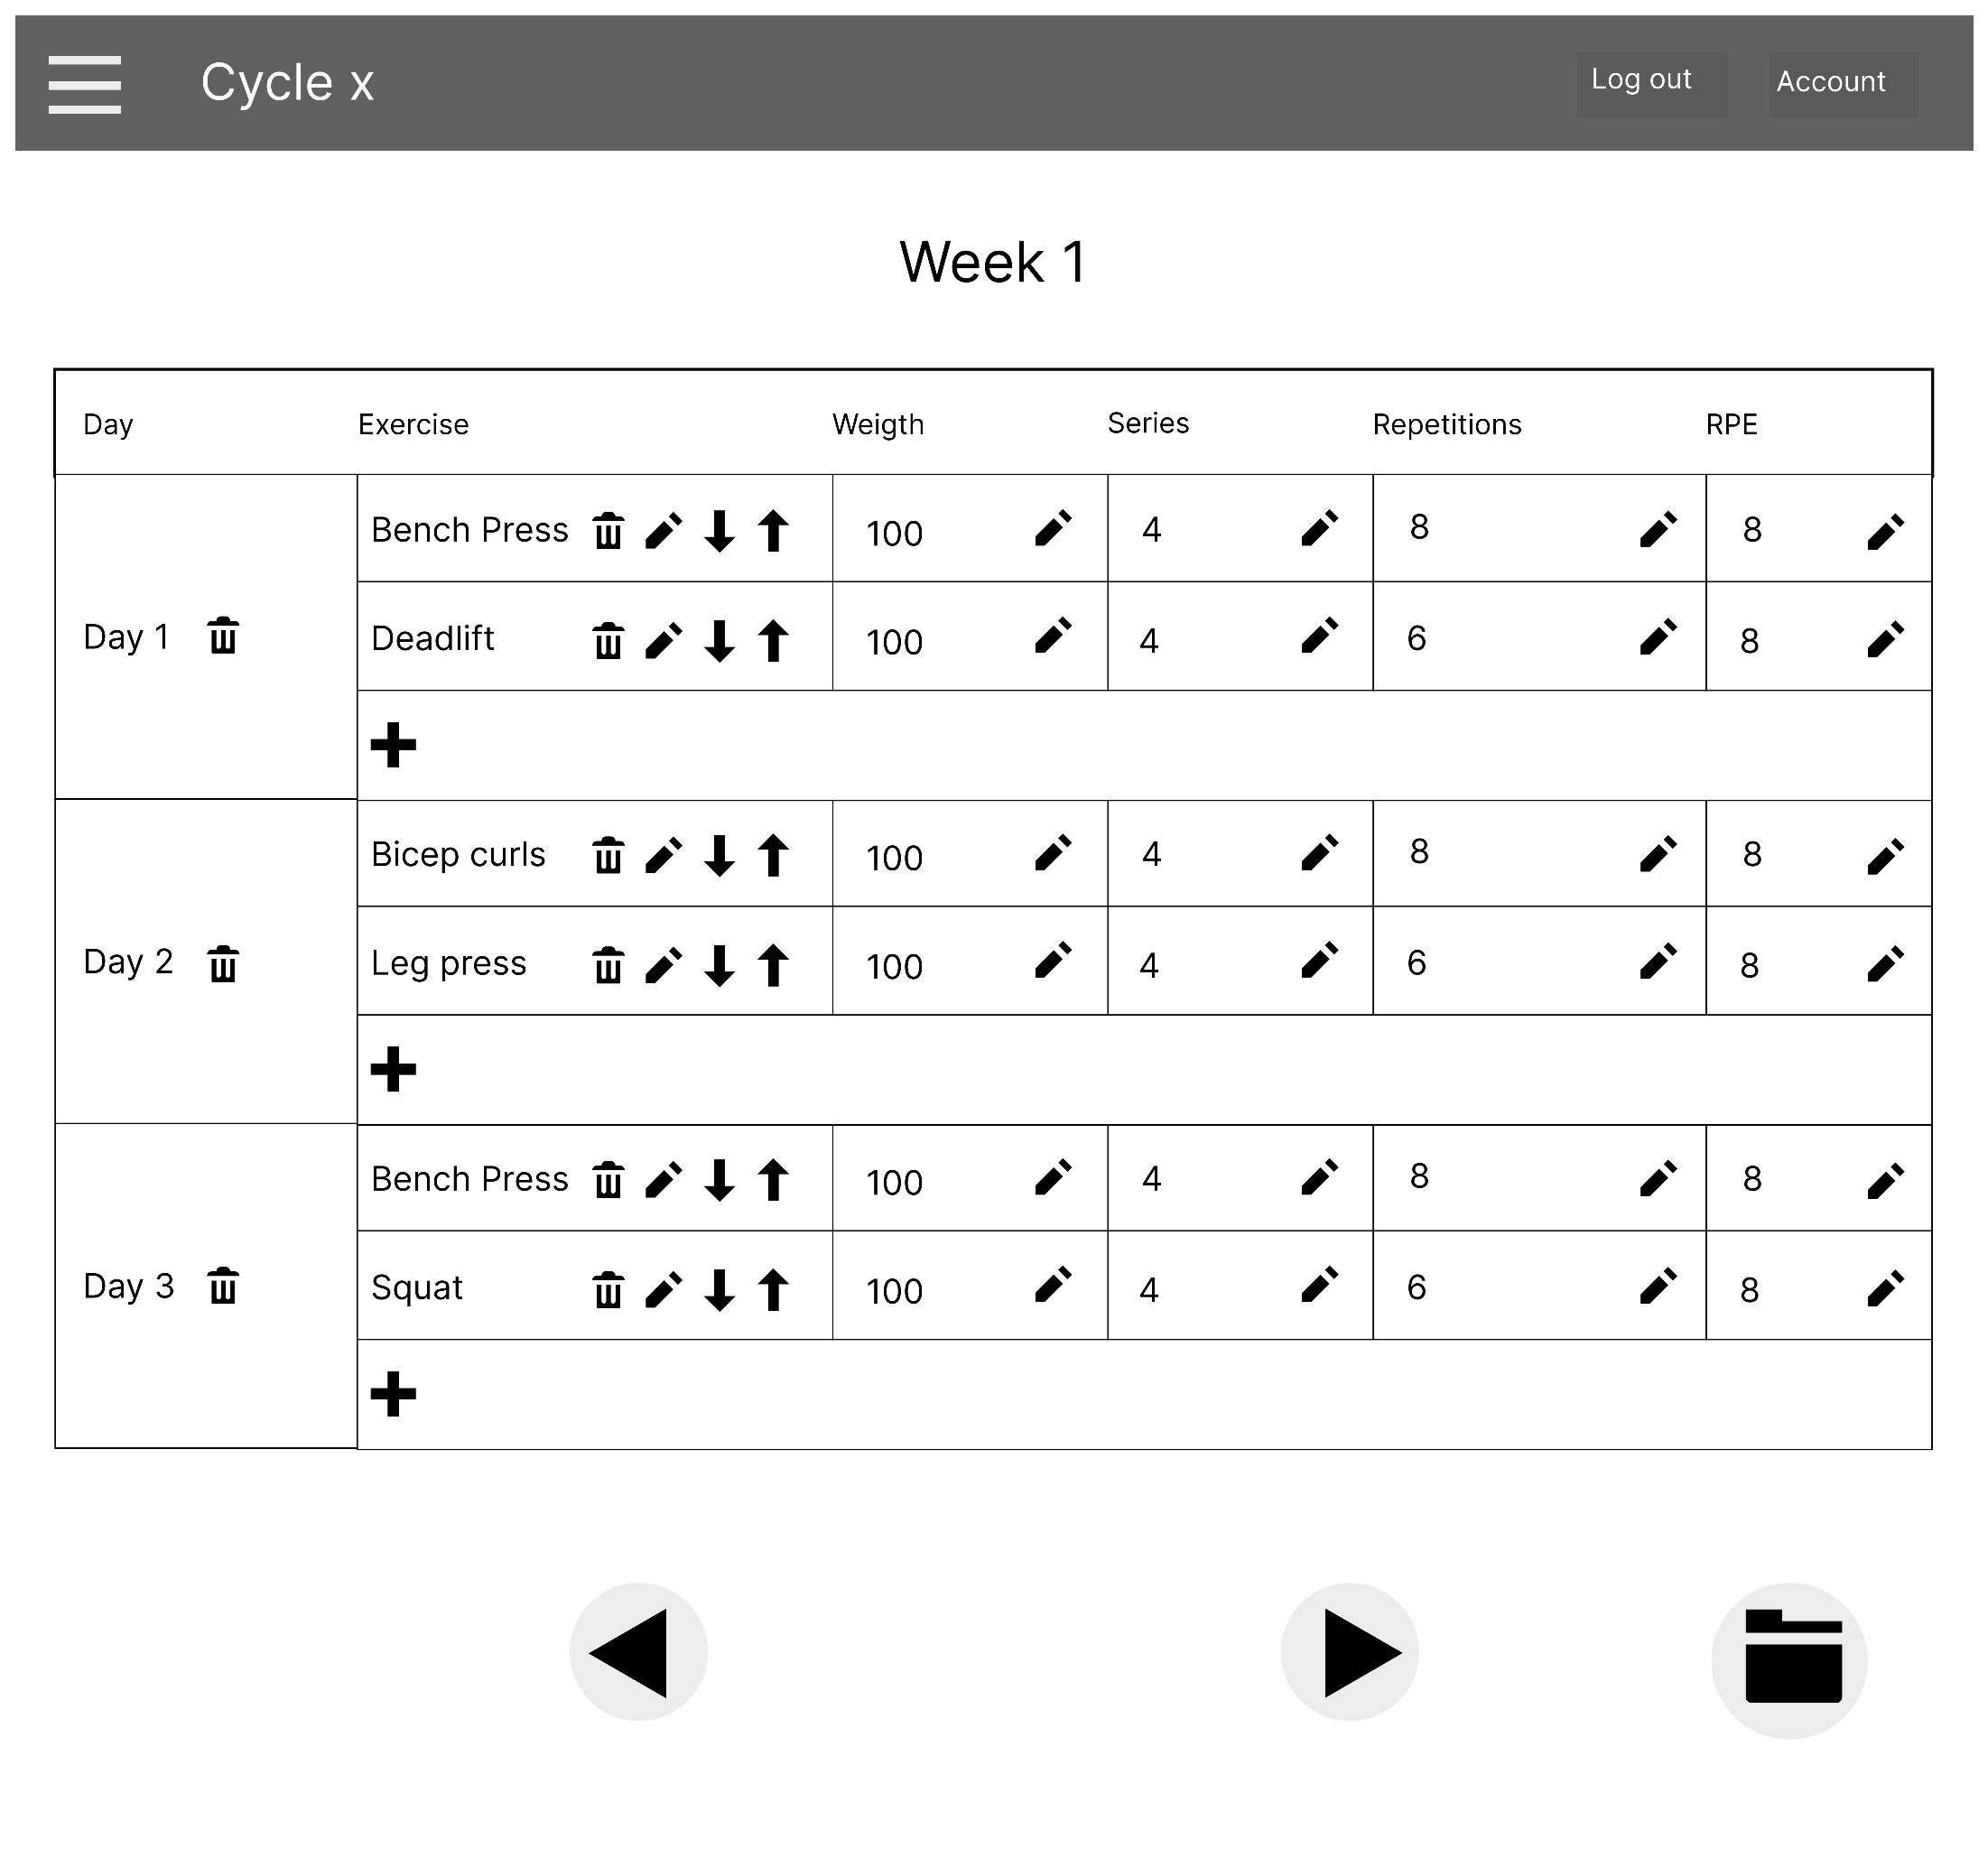
\includegraphics[width=0.7\linewidth]{workouttable}
}	\caption{Edzésterv oldal drótváza}
	\label{fig:workouttable}
\end{figure}

\subsection{Kliensek listázó oldala}
\begin{figure}[H]
	\centering
\fbox{	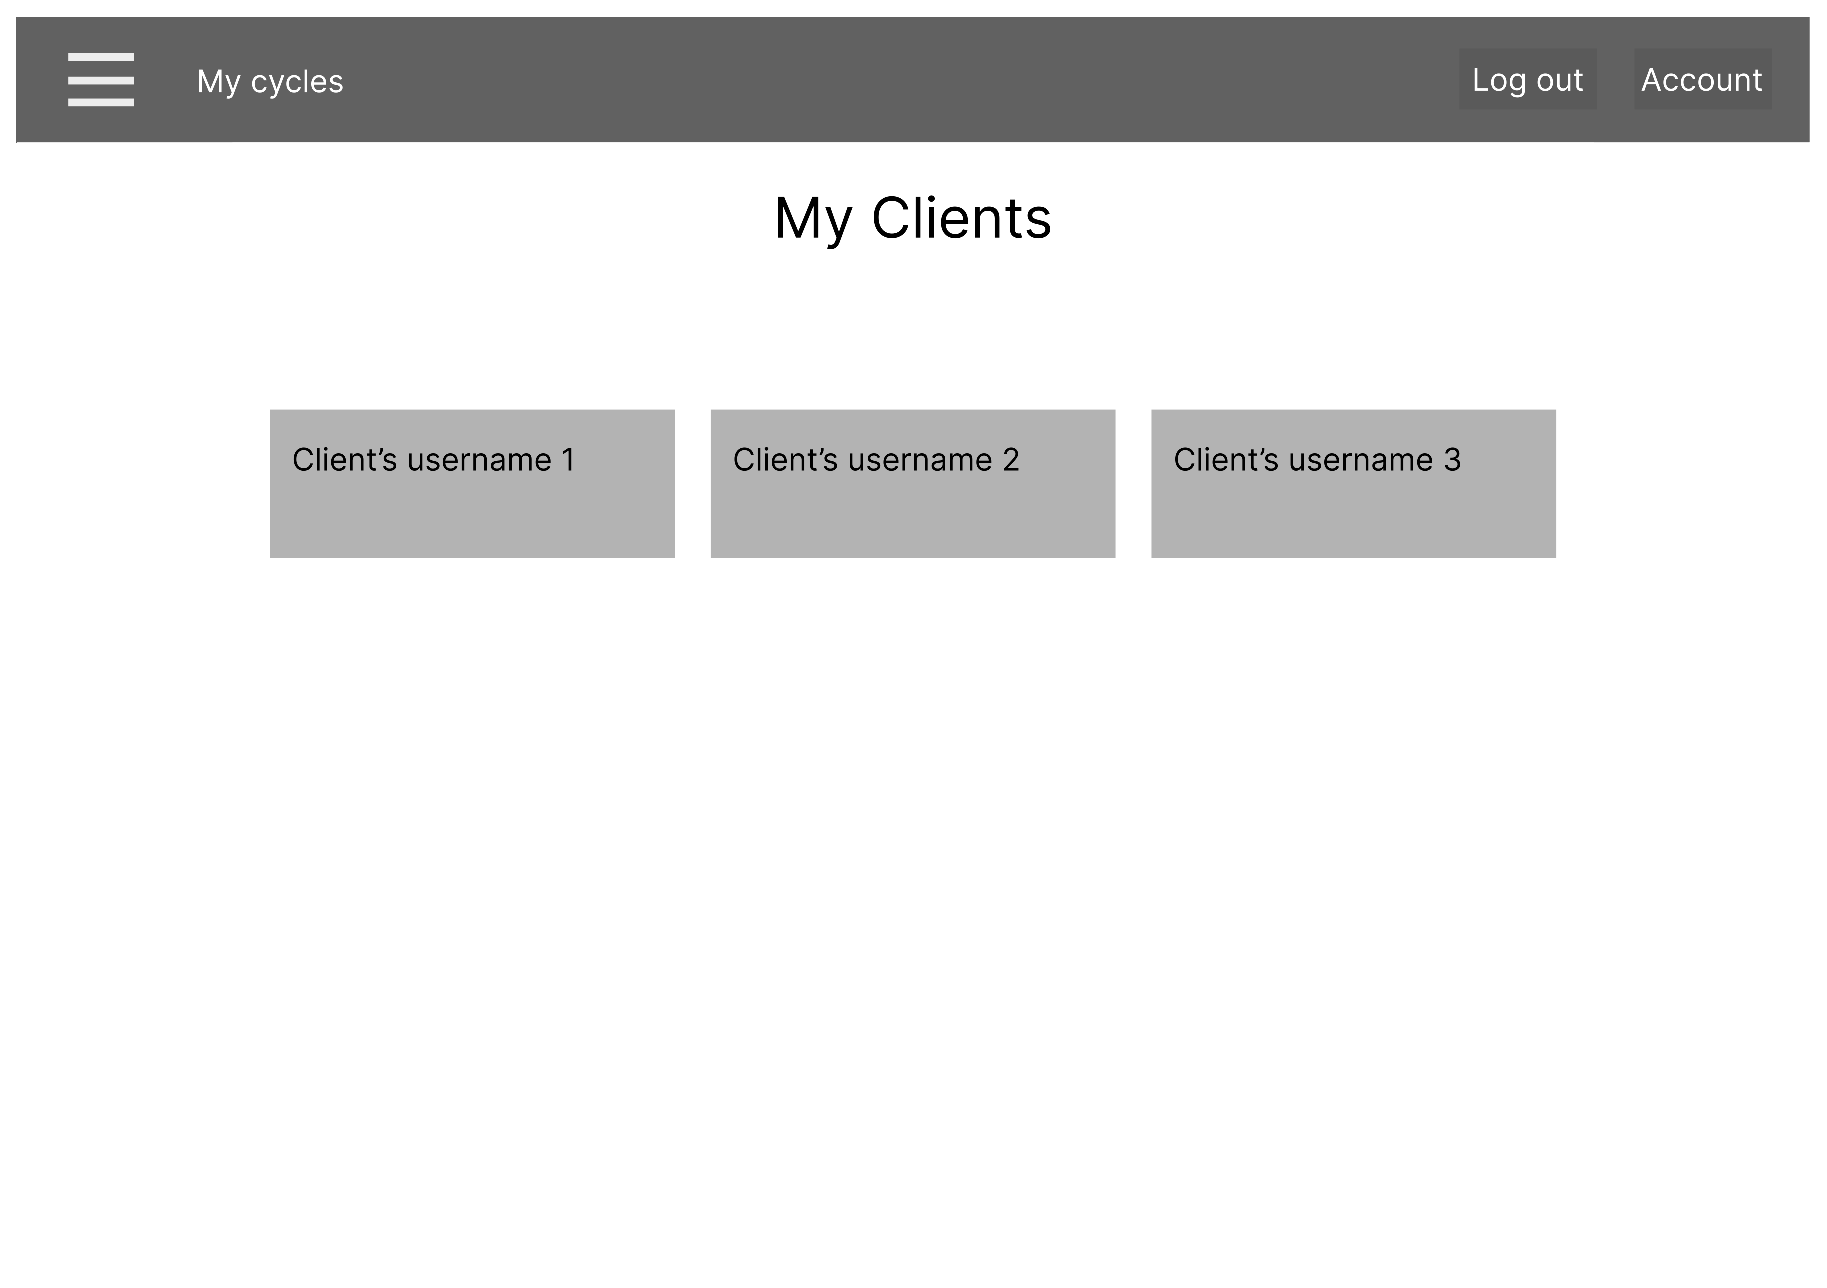
\includegraphics[width=0.8\linewidth]{clientspagewireframe}
}	\caption{Kliensek listázó oldal drótváza}
	\label{fig:clientspagewireframe}
\end{figure}

\subsection{Chat oldal}
\begin{figure}[H]
	\centering
\fbox{	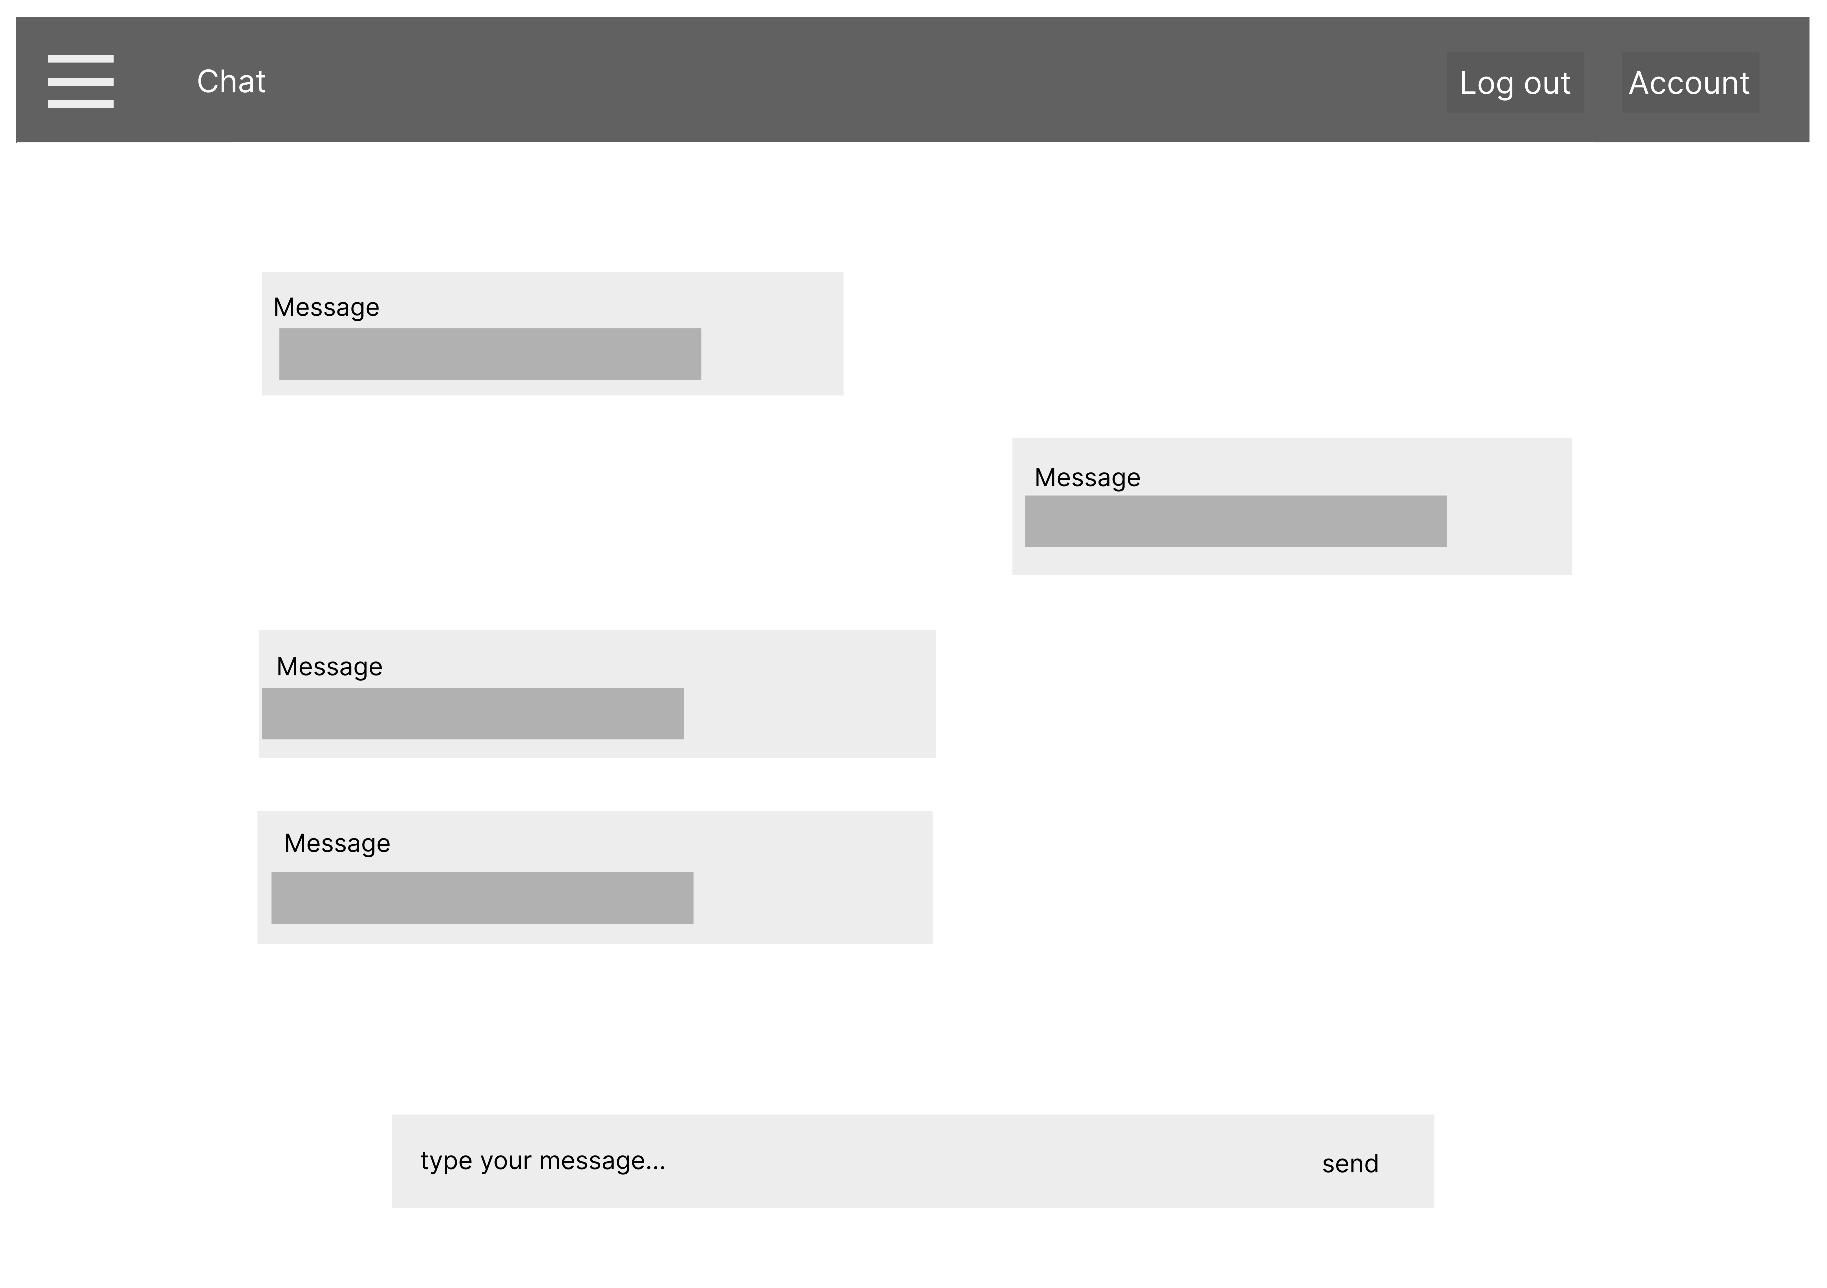
\includegraphics[width=0.8\linewidth]{chat}
}	\caption{Chat oldal drótváza}
	\label{fig:chat}
\end{figure}

\subsection{Profil beállítások oldal}
\begin{figure}[H]
	\centering
\fbox{	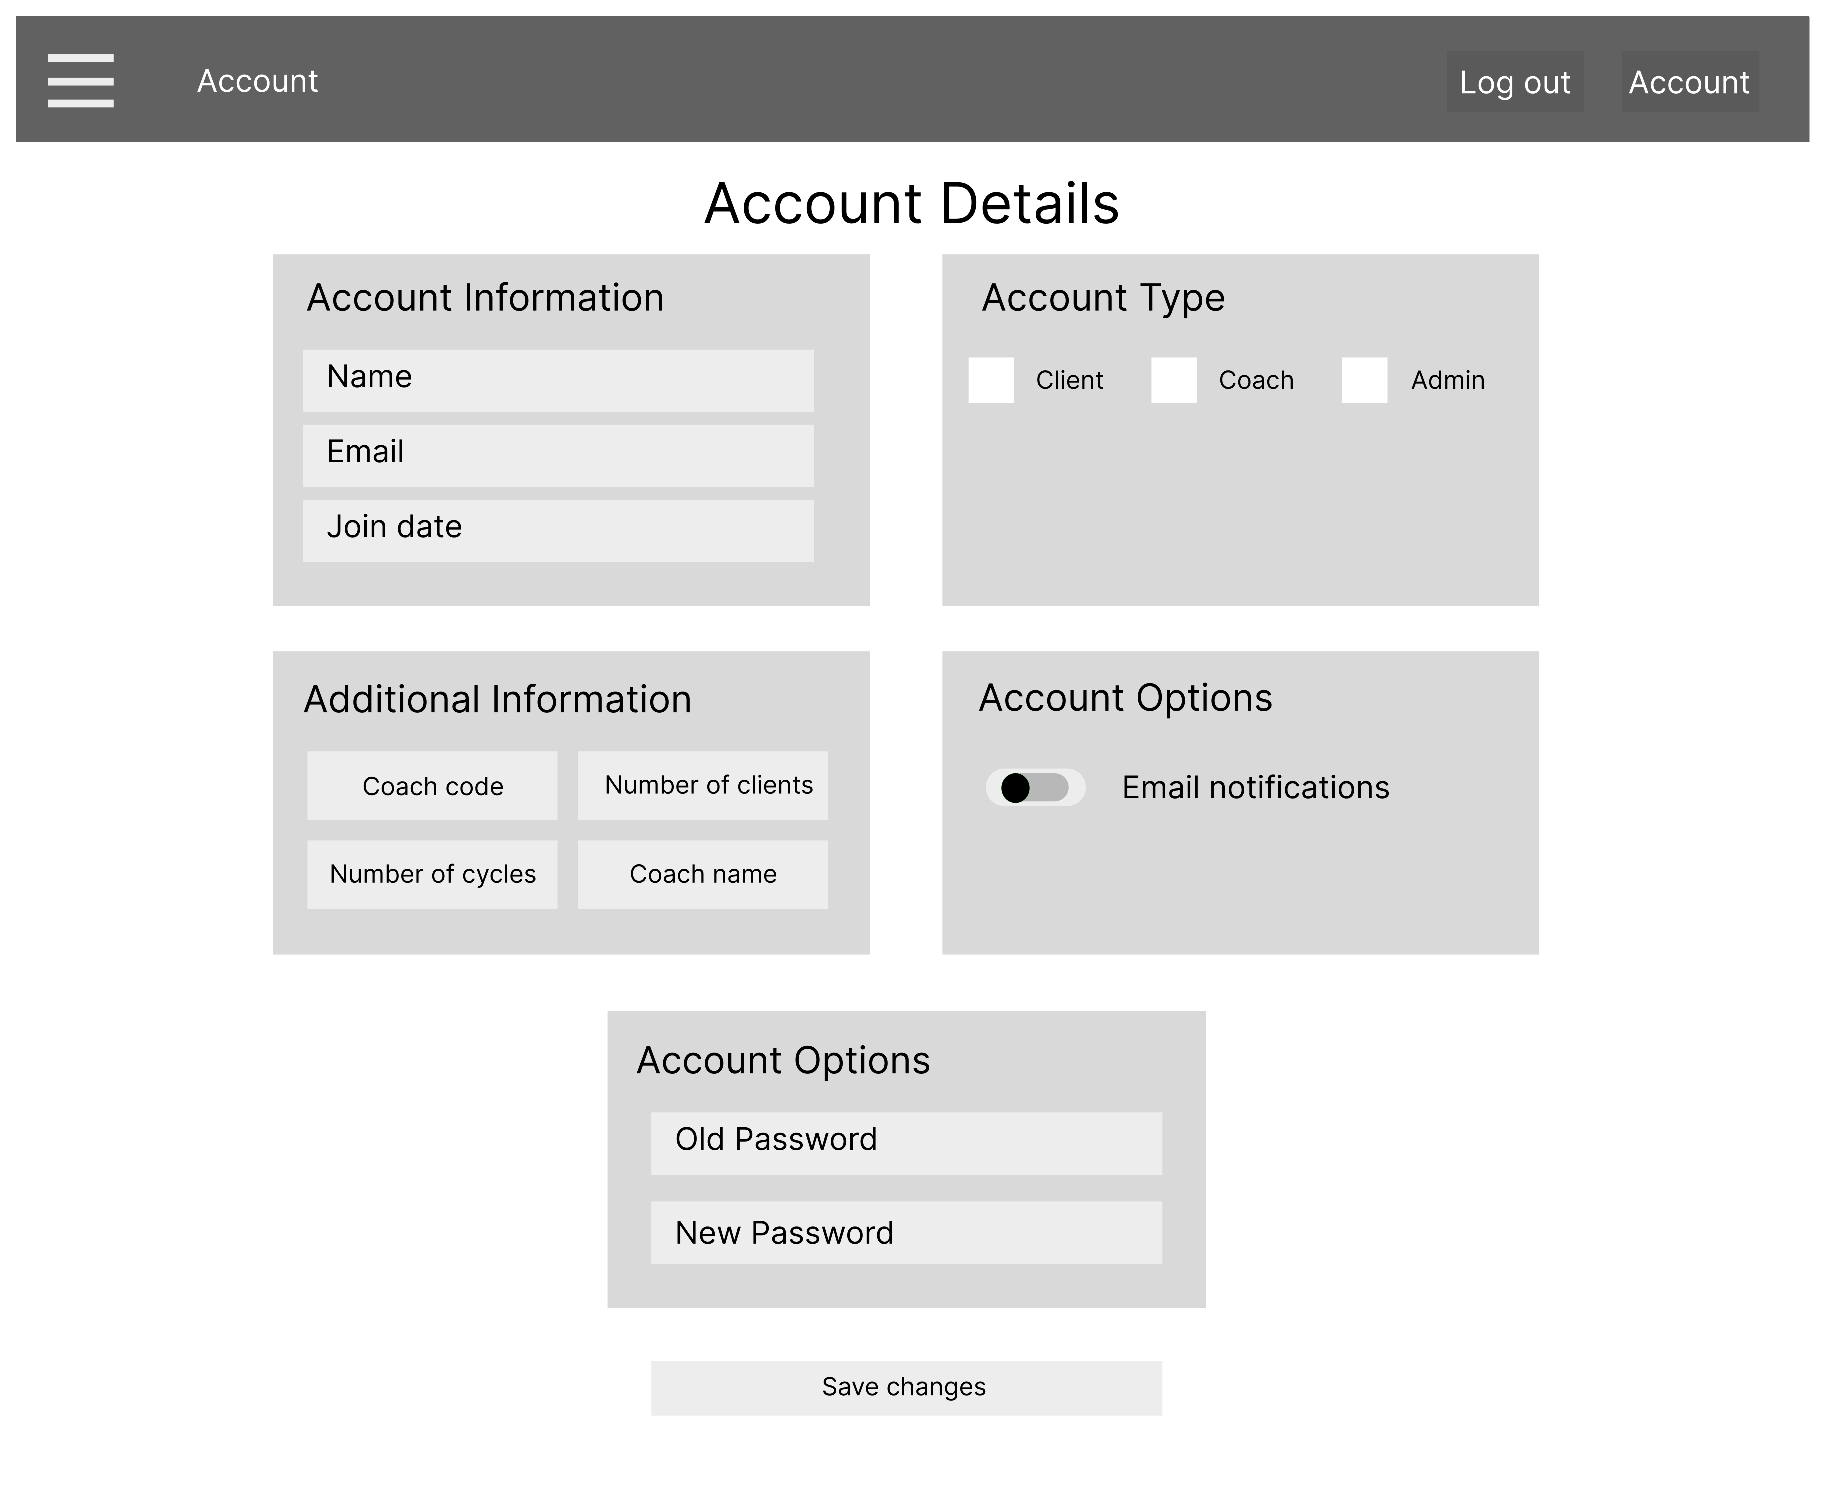
\includegraphics[width=0.8\linewidth]{account}
}	\caption{Profil beállítások oldal drótváza}
	\label{fig:account}
\end{figure}


\section{Program futtatása lokálisan}

A telepítési folyamatok során az alapértelmezett beállítások szerint haladunk, nem szükséges speciális beállítás egyik telepítőben sem.

\begin{enumerate}
	\item A mellékelt ZIP fájlt csomagoljuk ki egy tetszőleges könyvtárba
	\item Töltsük le a \href{https://www.mongodb.com/try/download/community}{MongoDB Community Server-t} (link). Válasszuk ki a megfelelő platformot és telepítési módszert, majd kattintsunk a "Download" gombra (\ref{fig:mongodbcommunityserver} ábra).
	\begin{figure}[H]
		\centering
		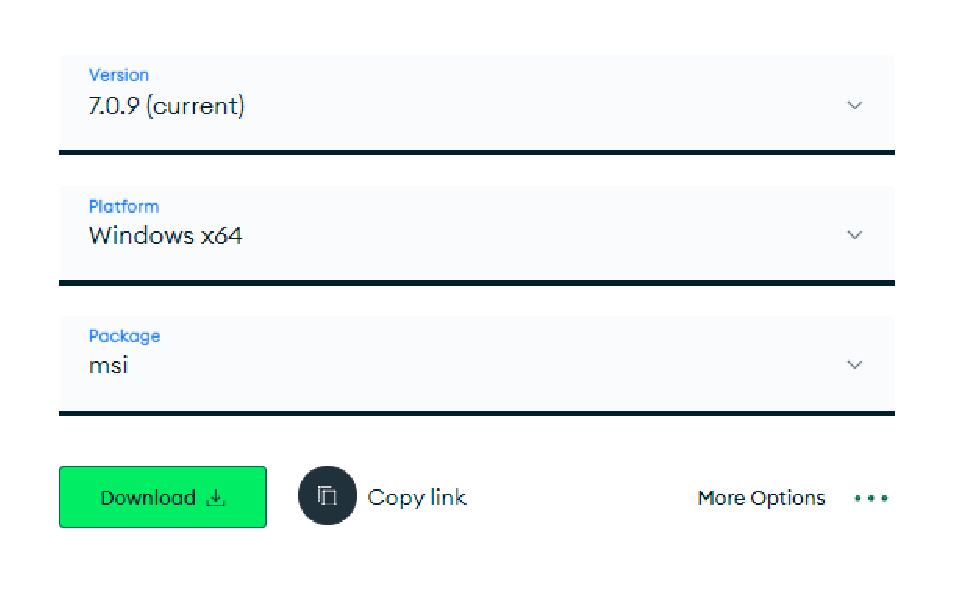
\includegraphics[width=0.65\linewidth]{mongodbcommunityserver}
		\caption{MongoDB Community Server letöltés}
		\label{fig:mongodbcommunityserver}
	\end{figure}
	\item Telepítsük a MongoDB Shell-t, illetve a MongoDB Compass Grafikai felhasználói felületet, igény szerint a következő linkről \url{https://www.mongodb.com/try/download/compass} a 2. pontban leírtakhoz hasonlóan.
	\item Programom NodeJs-t, illetve ennek csomagkezelőjét (NPM)-t használ. A \url{https://nodejs.org/en/download} oldalról töltsük le a NodeJs legfrisebb LTS verzióját, válasszuk ki az operációs rendszerünknek és igényeinknek megfelelő telepítési módot, majd kattintsunk a "Download" gombra (\ref{fig:nodejsdownload} ábra).
	\begin{figure}[H]
		\centering
		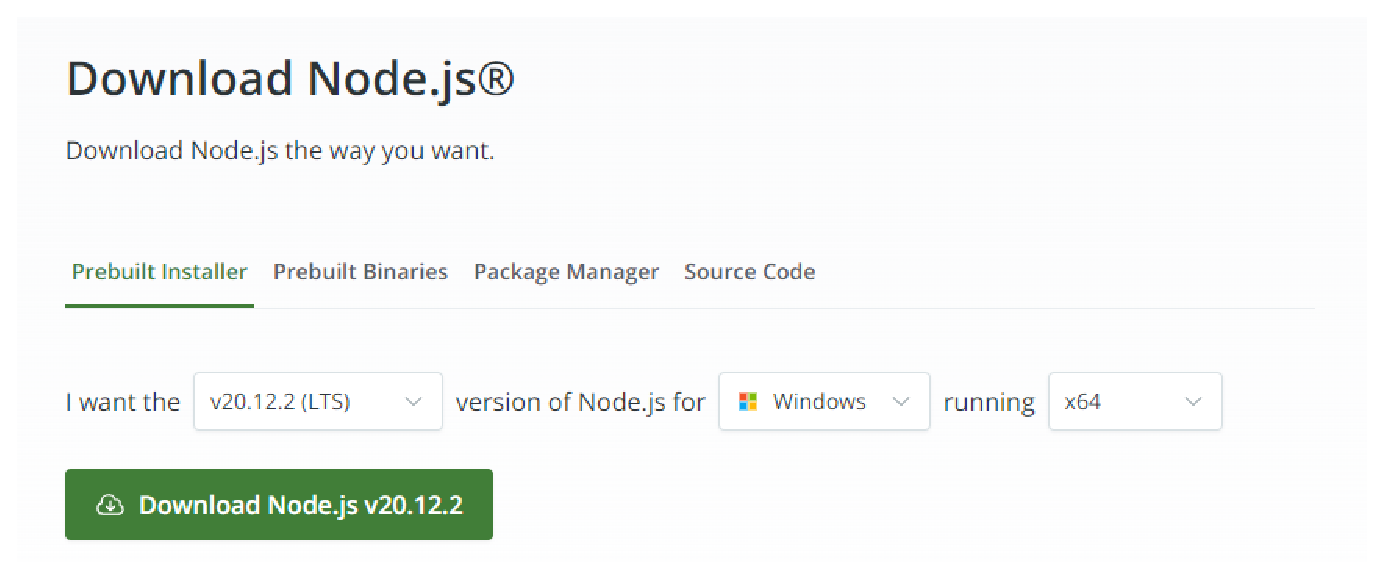
\includegraphics[width=0.7\linewidth]{nodejsdownload}
		\caption{NodeJs letöltés}
		\label{fig:nodejsdownload}
	\end{figure}

	\item Nyissunk meg egy-egy terminált a program kicsomagolt helyére, az első terminálban futtassunk le a \texttt{cd server}, a másodikban a \texttt{cd client} parancsot. Majd minkettőben az \texttt{npm i} parancsot, miután ezek lefutottak a \texttt{npm run dev} parancsot. Ezt követően győződjunk meg róla, hogy a szerver sikeresen csatlakozott az adatbázis szerverhez (A terminálon a "Server started on port 5000" üzenet jelzi). Ezután böngészőnkön csatlakozhatunk a kliens terminálján kiírt url-en keresztül (alapértelmezett esetben \url{http://localhost:5173/}).
\end{enumerate}


\section{Tesztelési terv}

A program tesztelése folyamán a User-story táblázatot használtam referenciaként és a táblázatban szereplő sorrend és sorszámok alapján teszteltem.

\begin{center}
	\begin{longtable}{ | p{0.06\textwidth} | p{0.2\textwidth} | p{0.52\textwidth} | p{0.12\textwidth} | }
			
			\hline
			\multicolumn{4}{|c|}{\textbf{As a látogató}}
			\\ \hline
			
			\# & Eset & Leírás & Eredmény
			\\ \hline \hline
			\endfirsthead % első oldal fejléce
			
			\hline
			\# & Eset & Leírás & Eredmény
			\\ \hline \hline
			\endhead % többi oldal fejléce
			
			\hline
			\endfoot % többi oldal lábléce
			
			\endlastfoot % utolsó oldal lábléce
			
			% Regisztracio

			\multirow{6}{=}{0.1.1 0.1.2 0.1.3} 
			& \multirow{6}{=}{Regisztráció} 
			& Nem bejelentkezett felhasználóknak helyesen megjelenik a kezdőlap 
			& OK \\
			\cline{3-4}
			& & A jobb felső sarokban található "Sign Up" gomb a regisztrációs oldalra irányít 
			& OK \\
			\cline{3-4}
			& & Regisztrációs oldal helyesen megjelenik 
			& OK \\
			\cline{3-4}
			& & Helyes adatokkal történő regisztráció után a fiók létrejön, majd a bejelentkezett felhasználó a kliens vagy edző kezdőlapra kerül 
			& OK \\
			\cline{3-4}
			& & Helytelen adatokkal való kitöltés után a megfelelő hibaüzenet megjelenik ha a küldés gombra kattintunk 
			& OK \\
			\cline{3-4}
			& & Helytelen adatokkal való kitöltés után nem jön létre felhasználói fiók
			& OK \\
			\hline

			\multirow{5}{=}{0.2.1 0.2.2 0.2.3} 
			& \multirow{5}{=}{Bejelentkezés} 
			& A jobb felső sarokban található "Login" gomb a bejelentkezés oldalra irányít 
			& OK \\
			\cline{3-4}
			& & Bejelentkezés oldal helyesen megjelenik 
			& OK \\
			\cline{3-4}
			& & Helyes adatokkal történő bejelentkezés után a bejelentkezett felhasználó a kliens vagy edző kezdőlapra kerül 
			& OK \\
			\cline{3-4}
			& & Helytelen adatokkal való kitöltés után a megfelelő hibaüzenet megjelenik ha a küldés gombra kattintunk 
			& OK \\
			\cline{3-4}
			& & Helytelen adatokkal való kitöltés után a bejelentkezés oldalon maradunk
			& OK \\
			\hline

			\caption{Látogató tesztelési táblázat}
			\label{tab:testlatogato}       
	\end{longtable}
\end{center}



\begin{center}
	\begin{longtable}{ | p{0.06\textwidth} | p{0.2\textwidth} | p{0.52\textwidth} | p{0.12\textwidth} | }
			
			\hline
			\multicolumn{4}{|c|}{\textbf{As a kliens}}
			\\ \hline
			
			\# & Eset & Leírás & Eredmény
			\\ \hline \hline
			\endfirsthead % első oldal fejléce
			
			\hline
			\# & Eset & Leírás & Eredmény
			\\ \hline \hline
			\endhead % többi oldal fejléce
			
			\hline
			\endfoot % többi oldal lábléce
			
			\endlastfoot % utolsó oldal lábléce
			

			\multirow{2}{=}{1.0.1 1.1.0} 
			& \multirow{2}{=}{Kliens kezdőlap} 
			& A kliens kezdőlap sikeresen megjelenik 
			& OK \\
			\cline{3-4}
			& & A "My Cycles" gomb a ciklusok listázó oldalra továbbít hiba nélkül 
			& OK \\
			\hline

			\multirow{4}{=}{1.1.0 1.1.1 1.1.2} 
			& \multirow{4}{=}{Ciklusok listázó oldala} 
			& A ciklusok listázó oldala megjelenik hiba nélkül 
			& OK \\
			\cline{3-4}
			& & Az oldalon a felhasználó összes ciklusa látható 
			& OK \\
			\cline{3-4}
			& & Egy aktív ciklus cellájára kattintva betölt az adott ciklushoz tartozó edzésterv 
			& OK \\
			\cline{3-4}
			& & Egy inaktív ciklus cellájára kattintva betölt az adott ciklushoz tartozó edzésterv
			& OK \\
			\hline

			\multirow{8}{=}{1.1.3 - 1.1.16} 
			& \multirow{8}{=}{Edzésterv oldal} 
			& Az edzésterv oldal hiba nélkül megjelenik 
			& OK \\
			\cline{3-4}
			& & Az oldalon az összes rögzített adat látható
			& OK \\
			\cline{3-4}
			& & A PDF letöltése gomb működik, megnyomása után letöltődik az edzésterv nyomtatható PDF formátumban 
			& OK \\
			\cline{3-4}
			& & Hetek közötti lapozás helyesen működik, az oldal alján található nyíl ikon irányába haladunk 
			& OK \\
			\cline{3-4}
			& & Ha elérünk a terv első hetéhez, a bal oldali nyíl gomb inaktív lesz
			& OK \\
			\cline{3-4}
			& & Ha elérünk a terv utolsó hetéhez, a jobb oldali nyíl gomb inaktív lesz
			& OK \\
			\cline{3-4}
			& & Módosítások után a mentés gomb aktív
			& OK \\
			\cline{3-4}
			& & Az aktív mentés gombra kattintás után az adatok helyesen mentésre kerülnek, ha az oldalról kilépünk majd vissza, helyesen megjelennek
			& OK \\
			\hline

			\pagebreak

			\multirow{4}{=}{1.1.4 - 1.1.6} 
			& \multirow{4}{=}{Súly módosító űrlap} 
			& A súly oszlopban lévő ceruza ikonra kattintva megnyílik a súly módosító űrlap
			& OK \\
			\cline{3-4}
			& & Súly módosítás valid értékkel helyesen megtörténik
			& OK \\
			\cline{3-4}
			& & Negatív vagy 10000-nél nagyobb szám megadása esetén hibaüzenetet kapunk
			& OK \\
			\cline{3-4}
			& & Hibás adatot nem tudunk elmenteni a súly módosító űrlapon
			& OK \\
			\hline


			\multirow{4}{=}{1.1.7 - 1.1.9} 
			& \multirow{4}{=}{Sorozat/ismétlés /RPE módosító űrlap}
			& Sorozat/ismétlés/RPE mezőkben a ceruza ikonra kattintva az adat módosító űrlap hiba nélkül megjelenik
			& OK \\
			\cline{3-4}
			& & A Sorozat/ismétlés/RPE módosító űrlapon valid értéket megadva az adat helyesen elmentődik
			& OK \\
			\cline{3-4}
			& & A Sorozat/ismétlés/RPE módosító űrlapon negatív vagy 100-nál nagyobb érték megadása esetén hibaüzenet jelenik meg
			& OK \\
			\cline{3-4}
			& & Hibás adatot nem tudunk elmenteni a Sorozat/ismétlés/RPE módosító űrlapon
			& OK \\
			\hline

			\multirow{5}{=}{1.2.0 1.2.1} 
			& \multirow{5}{=}{Chat oldal}
			& Chat oldal elérhető a navigációs menüből, hiba nélkül betölt
			& OK \\
			\cline{3-4}
			& & Korábbi üzenetek betöltődnek
			& OK \\
			\cline{3-4}
			& & Üzenet küldése során a tartalom mindkettő félnek megjelenik valódi időben
			& OK \\
			\cline{3-4}
			& & 255 karakterhossz felett nem tud a felhasználó üzenetet küldeni
			& OK \\
			\cline{3-4}
			& & Ha a beviteli mező üres, a küldés gomb inaktív
			& OK \\
			\hline

			\multirow{6}{=}{1.3.0 - 1.3.5} 
			& \multirow{6}{=}{Profil oldal}
			& Chat oldal elérhető a navigációs menüből vagy a jobb felső sarokban lévő gomb által, hiba nélkül betölt
			& OK \\
			\cline{3-4}
			& & A név mező módosítható, 20 karakterhosszig
			& OK \\
			\cline{3-4}
			& & Az értesítések állapotát módosítani tudja a felhasználó a csúszka segítségével
			& OK \\
			\cline{3-4}
			& & Az űrlapot csak a régi jelszó megadása után lehetséges elküldeni
			& OK \\
			\cline{3-4}
			& & Ha a megadott régi jelszó hibás, nem mentődik el semmilyen változtatás és hibaüzenet jelenik meg
			& OK \\
			\cline{3-4}
			& & Ha a megadott régi jelszó helyes, mentésre kerül a megadott információ
			& OK \\
			\hline

			\caption{Kliens tesztelési táblázat}
			\label{tab:testkliens}       
	\end{longtable}
\end{center}

\pagebreak

\begin{center}
	\begin{longtable}{ | p{0.06\textwidth} | p{0.2\textwidth} | p{0.52\textwidth} | p{0.12\textwidth} | }
			
			\hline
			\multicolumn{4}{|c|}{\textbf{As a edző}}
			\\ \hline
			
			\# & Eset & Leírás & Eredmény
			\\ \hline \hline
			\endfirsthead % első oldal fejléce
			
			\hline
			\# & Eset & Leírás & Eredmény
			\\ \hline \hline
			\endhead % többi oldal fejléce
			
			\hline
			\endfoot % többi oldal lábléce
			
			\endlastfoot % utolsó oldal lábléce

			\multirow{2}{=}{2.0.1 2.1.1} 
			& \multirow{2}{=}{Edző kezdőlap} 
			& Az edző kezdőlap sikeresen megjelenik 
			& OK \\
			\cline{3-4}
			& & A "My Clients" gomb a kliensek listázó oldalra továbbít hiba nélkül 
			& OK \\
			\hline
			
			\multirow{4}{=}{2.1.1 2.2.1} 
			& \multirow{4}{=}{Kliensek listázó oldala} 
			& A kliensek listázó oldala megjelenik hiba nélkül 
			& OK \\
			\cline{3-4}
			& & Az oldalon a felhasználó összes kliense látható 
			& OK \\
			\cline{3-4}
			& & Egy kliens cellájára kattintva betölt az adott kliens ciklusok listázó oldala
			& OK \\
			\cline{3-4}
			& & Egy kliens cellájában lévő chat ikonra kattintva betölt a két felhasználó közötti chat oldal
			& OK \\
			\hline

			\multirow{9}{=}{2.3.1 - 2.3.6} 
			& \multirow{9}{=}{Kliens ciklusainak listázó oldala} 
			& Adott kliens ciklusainak listázó oldala megjelenik, a kliens ciklusaival
			& OK \\
			\cline{3-4}
			& & Az oldalon a kliens összes ciklusa látható 
			& OK \\
			\cline{3-4}
			& & Ha aktív vagy inaktív ciklusra kattintunk, betölt a hozzájuk tartozó edzésterv oldal
			& OK \\
			\cline{3-4}
			& & Adott ciklus cellájában lévő törlés ikonra kattintva felugrik egy megerősítő ablak, annak elfogadása után a kiválasztott ciklus törlésre kerül
			& OK \\
			\cline{3-4}
			& & Adott ciklus cellájában lévő archiválás ikonra kattintva a ciklus aktivitási státusza megváltozik, átkerül a másik listába
			& OK \\
			\cline{3-4}
			& & A kék hátterű plusz gombra kattintva megjelenik a ciklus hozzáadása űrlap
			& OK \\
			\cline{3-4}
			& & Ciklus név megadása és az űrlap elküldése után rögzítésre kerül egy új, üres ciklus
			& OK \\
			\cline{3-4}
			& & Az új ciklus űrlapon a "Randomize Cycle" gombra kattintva az űrlap kibővül extra bemeneti mezőkkel
			& OK \\
			\cline{3-4}
			& & Az extra paraméterek megadása és az űrlap elküldése után helyesen legenerálódik a véletlenszerűen összeállított edzésterv, a megadott paraméterek szerint
			& OK \\
			\hline

			\multirow{16}{=}{2.3.7 - 2.3.25} 
			& \multirow{16}{=}{Kliens edzéstervének megtekintő/ módosító oldala} 
			& Megjelenik az edzésterv hiba nélkül, a megfelelő módosító gombokkal, helyes adatokkal
			& OK \\
			\cline{3-4}
			& & PDF letöltése gomb helyesen megjelenik és működik, a letöltött PDF helyes
			& OK \\
			\cline{3-4}
			& & Súly módosító űrlap helyesen megjelenik ha a súly oszlopban lévő ceruza ikonra kattintunk
			& OK \\
			\cline{3-4}
			& & Súlyt módosítani csak helyes bemeneti adatokkal enged az űrlap
			& OK \\
			\cline{3-4}
			& & Űrlap elküldése után megváltozik az adott gyakorlathoz tartozó súly adat
			& OK \\
			\cline{3-4}
			& & Gyakorlatot törölni tudunk a törlés gombbal
			& OK \\
			\cline{3-4}
			& & Gyakorlat módosító űrlap helyesen megjelenik a megfelelő ceruza ikonra kattintva, műküdése helyes és a bemeneti mezők ellenőrizve vannak
			& OK \\
			\cline{3-4}
			& & Új gyakorlat űrlap helyesen megjelenik a megfelelő plusz ikonra kattintva, műküdése helyes és a bemeneti mezők ellenőrizve vannak
			& OK \\
			\cline{3-4}
			& & Sorozat/ismétlés/RPE módosító űrlap helyesen megjelenik a megfelelő plusz ikonra kattintva, műküdése helyes és a bemeneti mezők ellenőrizve vannak
			& OK \\
			\cline{3-4}
			& & Új gyakorlat hozzáadása vagy meglévő gyakorlat szerkesztése után az űrlapon elküldött adatok helyesen megjelennek a táblázatban
			& OK \\
			\cline{3-4}
			& & Edzésnap törlése esetén az adat helyesen törlődik a táblázatból, a hozzá tartozó gyakorlatokkal
			& OK \\
			\cline{3-4}
			& & Edzésnap hozzáadása rendesen működik a megfelelő ikonra kattintva
			& OK \\
			\cline{3-4}
			& & Hét törlése megfelelően működik a megfelelő ikonra kattintva
			& OK \\
			\cline{3-4}
			& & Hét hozzáadása megfelelően működik a megfelelő ikonra kattintva, amely csak akkor jelenik meg a hetek közötti jobbra lapozás ikon helyén, ha az edzésterv utolsó hetén van a nézetünk
			& OK \\
			\cline{3-4}
			& & Módosítások után a mentés gomb aktív
			& OK \\
			\cline{3-4}
			& & Az aktív mentés gombra kattintás után az adatok helyesen mentésre kerülnek, ha az oldalról kilépünk majd vissza, helyesen megjelennek
			& OK \\
			\hline

			\multirow{6}{=}{2.4.1 - 2.4.6} 
			& \multirow{6}{=}{Profil oldal}
			& Chat oldal elérhető a navigációs menüből vagy a jobb felső sarokban lévő gomb által, hiba nélkül betölt
			& OK \\
			\cline{3-4}
			& & A név mező módosítható, 20 karakterhosszig
			& OK \\
			\cline{3-4}
			& & Az értesítések állapotát módosítani tudja a felhasználó a csúszka segítségével
			& OK \\
			\cline{3-4}
			& & Az űrlapot csak a régi jelszó megadása után lehetséges elküldeni
			& OK \\
			\cline{3-4}
			& & Ha a megadott régi jelszó hibás, nem mentődik el semmilyen változtatás és hibaüzenet jelenik meg
			& OK \\
			\cline{3-4}
			& & Ha a megadott régi jelszó helyes, mentésre kerül a megadott információ
			& OK \\
			\hline

			\caption{Edző tesztelési táblázat}
			\label{tab:testedzo}       
	\end{longtable}
\end{center}



\begin{center}
	\begin{longtable}{ | p{0.06\textwidth} | p{0.2\textwidth} | p{0.52\textwidth} | p{0.12\textwidth} | }
			
			\hline
			\multicolumn{4}{|c|}{\textbf{As an adminisztrátor}}
			\\ \hline
			
			\# & Eset & Leírás & Eredmény
			\\ \hline \hline
			\endfirsthead % első oldal fejléce
			
			\hline
			\# & Eset & Leírás & Eredmény
			\\ \hline \hline
			\endhead % többi oldal fejléce
			
			\hline
			\endfoot % többi oldal lábléce
			
			\endlastfoot % utolsó oldal lábléce

			\multirow{1}{=}{3.0.1} 
			& \multirow{1}{=}{Adminisztrátor kezdőlap} 
			& Az adminisztrátor kezdőlap sikeresen megjelenik 
			& OK \\
			\hline
			
			\multirow{6}{=}{3.1.1 - 3.1.8} 
			& \multirow{6}{=}{Felhasználók listázó oldala} 
			& Felhasználók listázó oldala helyesen megjelenik, az összes regisztrált felhasználóval
			& OK \\
			\cline{3-4}
			& & A lista szűrhető az oldal tetején található kiválasztó által
			& OK \\
			\cline{3-4}
			& & Felhasználók törlése helyesen működik a "Delete User" gombra kattintva
			& OK \\
			\cline{3-4}
			& & Adminisztrátor felhasználók nem törölhetőek ezen a felületen
			& OK \\
			\cline{3-4}
			& & Edző fiók kliensei megtekinthetőek a lenyitható lista segítségével, helyesen megjelennek
			& OK \\
			\cline{3-4}
			& & Kliensek törölhetőek egy edző listájából a "Delete Client" gombra kattintva
			& OK \\
			\hline

			\multirow{6}{=}{3.2.1 - 3.2.5} 
			& \multirow{6}{=}{Profil oldal}
			& Chat oldal elérhető a navigációs menüből vagy a jobb felső sarokban lévő gomb által, hiba nélkül betölt
			& OK \\
			\cline{3-4}
			& & A név mező módosítható, 20 karakterhosszig
			& OK \\
			\cline{3-4}
			& & Az értesítések állapotát módosítani tudja a felhasználó a csúszka segítségével
			& OK \\
			\cline{3-4}
			& & Az űrlapot csak a régi jelszó megadása után lehetséges elküldeni
			& OK \\
			\cline{3-4}
			& & Ha a megadott régi jelszó hibás, nem mentődik el semmilyen változtatás és hibaüzenet jelenik meg
			& OK \\
			\cline{3-4}
			& & Ha a megadott régi jelszó helyes, mentésre kerül a megadott információ
			& OK \\
			\hline

			\caption{Adminisztrátor tesztelési táblázat}
			\label{tab:testadmin}       
	\end{longtable}
\end{center}


\subsection{Tesztelés alapján levont következtetések}

A program tesztelése során kiderült, hogy nem minden űrlap volt megfelelően ellenőrizve a bemenet helyessége szempontból. Például volt olyan szöveges bevitel, amelynek nem volt korlátozva a maximális hossza, így okozhatott volna hibákat működés során. Az összes ilyen elmaradást javítottam, növelve a program biztonságát.

\bigskip

A Chat felületen is korlátoztam a maximálisan eltárolt üzenetek mennyiségét, hiszen ha korlátlanul tároljuk ezeket megfelelő bővíthető tárhely nélkül, elég nagy adatmennyiség során az adatbázisban túlcsordulásos hiba léphet fel. 

\cleardoublepage

% \chapter{Conclusion}
\label{ch:sum}

Lorem ipsum dolor sit amet, consectetur adipiscing elit. In eu egestas mauris. Quisque nisl elit, varius in erat eu, dictum commodo lorem. Sed commodo libero et sem laoreet consectetur. Fusce ligula arcu, vestibulum et sodales vel, venenatis at velit. Aliquam erat volutpat. Proin condimentum accumsan velit id hendrerit. Cras egestas arcu quis felis placerat, ut sodales velit malesuada. Maecenas et turpis eu turpis placerat euismod. Maecenas a urna viverra, scelerisque nibh ut, malesuada ex.

Aliquam suscipit dignissim tempor. Praesent tortor libero, feugiat et tellus porttitor, malesuada eleifend felis. Orci varius natoque penatibus et magnis dis parturient montes, nascetur ridiculus mus. Nullam eleifend imperdiet lorem, sit amet imperdiet metus pellentesque vitae. Donec nec ligula urna. Aliquam bibendum tempor diam, sed lacinia eros dapibus id. Donec sed vehicula turpis. Aliquam hendrerit sed nulla vitae convallis. Etiam libero quam, pharetra ac est nec, sodales placerat augue. Praesent eu consequat purus.

% \cleardoublepage

\chapter{Összefoglalás}
\label{ch:osszefoglalas}

Programom írása során az összes tervezett funkció megvalósításra került, összességében elégedett vagyok a végeredménnyel. A feladat komplexitása a számítottnál nagyobbnak bizonyult, ugyanis a szoftver minden részében volt olyan dolog, amivel még nem találkoztam. Egyetemi tanulmányaim során alap szinten megismerkedtem a React és a Node.js keretrendszerekkel, azonban a szakdolgozat írása közben mélyebb betekintést nyertem ezekbe a technológiákba. Számos új és eddig ismeretlen függvénykönyvtárat is alkalmaztam, például a Material UI-t. Ennek köszönhetően a jövőbeli webfejlesztési projekteim során magabiztosan fogok mozogni a React és Node.js környezetében.


% Szakdolgozatom írása során viszont nagyon sok új tapasztalatot szereztem ezekkel a technológiákkal kapcsolatban. Több új, számomra eddig ismeretlen függvénykönyvtárat is igénybe vettem, mint például a Material UI. Ennek köszönhetően jövőbeli webbel kapcsolatos projekteim feljesztése során sokkal otthonosabban fogom magamat érezni a React és NodeJs világában.

\bigskip

Az architektúrát szerintem sikerült jól rétegelni különböző részekre, amely a választott keretrendszereknek részében köszönhető (a szerver és kliens oldal két, teljesen különálló szerveren fut), viszont ezen felül a könyvtár struktúrát és az üzleti logika szétválasztását is igyekeztem minél áltáthatóbban rendezni és elégedett vagyok az eredménnyel.

\bigskip

Következő webes projektemnél kevesebb hangsúlyt fektetnék a kliensoldal fejlesztésére az elején, mert nagyobb újraformázásokra volt szükség amikor a kliens- és szerveroldalt összekötöttem egymással. Ezért érdemesebb lett volna a két progamrészen párhuzamosan dolgozni.

\pagebreak

\section{Továbbfejlesztési lehetőségek}

Programomat úgy építettem fel, hogy könnyedén bővíthető legyen a felhasználói interfész. Új funkciókat, például egy táplálkozás követő funkciót, vagy edzéssel kapcsolatos statisztikákat hozzáadni nem járna refaktorálásokkal.

\bigskip

Ezek mellett esetleg egy natív telefonos applikáció készítése a jobb felhasználói élményért is egy továbbfejlesztési lehetőség lenne. A webes alkamazásom egy előnye, hogy számítógépen és mobil eszközökön is egyaránt működik.


\cleardoublepage

% Acknowledgements (optional) - in case your thesis received funding or would like to express special thanks to someone
% \chapter*{\acklabel}
% \addcontentsline{toc}{chapter}{\acklabel}
% Amennyiben a szakdolgozati / diplomamunka projekted pénzügyi támogatást kapott egy projektből vagy az egyetemtől, jellemzően kötelező feltüntetni a dolgozatban is. A dolgozat elkészítéséhez segítséget nyújtó oktatók, hallgatótársak, kollégák felé is nyilvánítható külön köszönet.

% Appendices (optional) - useful for detailed information in long tables, many and/or large figures, etc.
% \appendix
% \chapter{Szimulációs eredmények}
\label{appx:simulation}

Lorem ipsum dolor sit amet, consectetur adipiscing elit. Pellentesque facilisis in nibh auctor molestie. Donec porta tortor mauris. Cras in lacus in purus ultricies blandit. Proin dolor erat, pulvinar posuere orci ac, eleifend ultrices libero. Donec elementum et elit a ullamcorper. Nunc tincidunt, lorem et consectetur tincidunt, ante sapien scelerisque neque, eu bibendum felis augue non est. Maecenas nibh arcu, ultrices et libero id, egestas tempus mauris. Etiam iaculis dui nec augue venenatis, fermentum posuere justo congue. Nullam sit amet porttitor sem, at porttitor augue. Proin bibendum justo at ornare efficitur. Donec tempor turpis ligula, vitae viverra felis finibus eu. Curabitur sed libero ac urna condimentum gravida. Donec tincidunt neque sit amet neque luctus auctor vel eget tortor. Integer dignissim, urna ut lobortis volutpat, justo nunc convallis diam, sit amet vulputate erat eros eu velit. Mauris porttitor dictum ante, commodo facilisis ex suscipit sed.

Sed egestas dapibus nisl, vitae fringilla justo. Donec eget condimentum lectus, molestie mattis nunc. Nulla ac faucibus dui. Nullam a congue erat. Ut accumsan sed sapien quis porttitor. Ut pellentesque, est ac posuere pulvinar, tortor mauris fermentum nulla, sit amet fringilla sapien sapien quis velit. Integer accumsan placerat lorem, eu aliquam urna consectetur eget. In ligula orci, dignissim sed consequat ac, porta at metus. Phasellus ipsum tellus, molestie ut lacus tempus, rutrum convallis elit. Suspendisse arcu orci, luctus vitae ultricies quis, bibendum sed elit. Vivamus at sem maximus leo placerat gravida semper vel mi. Etiam hendrerit sed massa ut lacinia. Morbi varius libero odio, sit amet auctor nunc interdum sit amet.

Aenean non mauris accumsan, rutrum nisi non, porttitor enim. Maecenas vel tortor ex. Proin vulputate tellus luctus egestas fermentum. In nec lobortis risus, sit amet tincidunt purus. Nam id turpis venenatis, vehicula nisl sed, ultricies nibh. Suspendisse in libero nec nisi tempor vestibulum. Integer eu dui congue enim venenatis lobortis. Donec sed elementum nunc. Nulla facilisi. Maecenas cursus id lorem et finibus. Sed fermentum molestie erat, nec tempor lorem facilisis cursus. In vel nulla id orci fringilla facilisis. Cras non bibendum odio, ac vestibulum ex. Donec turpis urna, tincidunt ut mi eu, finibus facilisis lorem. Praesent posuere nisl nec dui accumsan, sed interdum odio malesuada.
% \cleardoublepage

% Bibliography (mandatory)
\phantomsection
\addcontentsline{toc}{chapter}{\biblabel}
\printbibliography[title=\biblabel]
\cleardoublepage

% List of figures (optional) - useful over 3-5 figures
\phantomsection
\addcontentsline{toc}{chapter}{\lstfigurelabel}
\listoffigures
\cleardoublepage

% List of tables (optional) - useful over 3-5 tables
% \phantomsection
% \addcontentsline{toc}{chapter}{\lsttablelabel}
% \listoftables
% \cleardoublepage

% List of algorithms (optional) - useful over 3-5 algorithms
% \phantomsection
% \addcontentsline{toc}{chapter}{\lstalgorithmlabel}
% \listofalgorithms
% \cleardoublepage

% List of codes (optional) - useful over 3-5 code samples
% \phantomsection
% \addcontentsline{toc}{chapter}{\lstcodelabel}
% \lstlistoflistings
% \cleardoublepage

% List of symbols (optional)
%\printnomenclature

\end{document}
